% =====================================================================
%  Anatomía de un LLM — Fase 0 — Módulo 0.2
%  Conjuntos, funciones y relaciones
%  Compilar: latexmk -r ../latexmkrc P02-conjuntos-funciones.tex
% =====================================================================
\documentclass[11pt,a4paper,twoside,openany]{book}
\usepackage{../estilo-apuntes}

\newcommand{\ApuntesCurso}{Anatomía de un LLM}
\newcommand{\ApuntesModulo}{Módulo 0.2}

% --- Notación propia del módulo -------------------------------------------
\newcommand{\N}{\mathbb{N}}
\newcommand{\Z}{\mathbb{Z}}
\newcommand{\Q}{\mathbb{Q}}
\newcommand{\Pa}{\mathcal{P}}
\newcommand{\id}{\mathrm{id}}
\newcommand{\cad}[1]{\texttt{#1}}
\newcommand{\vacia}{\varepsilon}
\newcommand{\dsim}{\mathbin{\triangle}}

\hypersetup{pdftitle={Módulo 0.2. Conjuntos, funciones y relaciones},pdfauthor={Anatomía de un LLM}}

\begin{document}
\frontmatter
% ------------------------------------------------------------------ Portada
\begin{titlepage}
\centering
\vspace*{2.5cm}
{\large\scshape Anatomía de un LLM}\par
\vspace{0.4cm}
{\normalsize Fundamentos matemáticos de los modelos de lenguaje}\par
\vspace{2.2cm}
\rule{\textwidth}{0.8pt}\par\vspace{0.5cm}
{\small\scshape Fase 0 \textperiodcentered\ Preliminares matemáticos}\par\vspace{0.3cm}
{\Huge\bfseries Módulo 0.2\par}\vspace{0.3cm}
{\LARGE Conjuntos, funciones y relaciones\par}
\vspace{0.5cm}\rule{\textwidth}{0.4pt}\par
\vspace{1.6cm}
{\large Apuntes del curso}\par
\vfill
{\small Edición de octubre de 2026}\par
\end{titlepage}

% ------------------------------------------------------- Presentación
\chapter*{Presentación del módulo}
\addcontentsline{toc}{chapter}{Presentación del módulo}
\markboth{Presentación del módulo}{}

Conjuntos, funciones y relaciones forman el lenguaje en el que se escribe el resto del curso. Un vocabulario es un conjunto finito; un tokenizador es una función que debe ser inyectiva para que el texto pueda recuperarse; una red neuronal es una composición de funciones; la máscara causal de un Transformer codifica una relación de orden entre posiciones. Este módulo repasa esos conceptos desde el nivel de bachillerato con el rigor de un primer curso universitario de matemática discreta, y pone el acento en \emph{demostrar}: que dos conjuntos son iguales, que una función es inyectiva o sobreyectiva, que una relación es de equivalencia o que un conjunto no es numerable.

\section*{Objetivos}
Al finalizar el módulo, el estudiante debe ser capaz de:
\begin{enumerate}[label=\arabic*.]
  \item operar con conjuntos (unión, intersección, diferencia, complemento, partes, producto cartesiano) y demostrar igualdades de conjuntos por doble inclusión;
  \item manejar con precisión los conceptos de función, dominio, codominio, recorrido, imagen y preimagen, y demostrar sus propiedades;
  \item decidir y demostrar si una función es inyectiva, sobreyectiva o biyectiva, tanto para funciones reales como para funciones entre enteros, conjuntos finitos y cadenas;
  \item componer funciones, calcular inversas y demostrar cómo se transmiten la inyectividad y la sobreyectividad a través de la composición;
  \item reconocer relaciones de equivalencia y de orden, describir sus clases y particiones y dibujar diagramas de Hasse;
  \item comparar cardinales, aplicar el principio del palomar, demostrar que un conjunto es numerable y usar el argumento diagonal de Cantor.
\end{enumerate}

\section*{Requisitos previos}
Matemáticas de bachillerato: números enteros, racionales y reales, funciones reales elementales (polinómicas, racionales, exponencial y logaritmo), resolución de ecuaciones y desigualdades. Se usan la lógica proposicional y las técnicas de demostración (directa, por contrarrecíproco, por reducción al absurdo e inducción) del módulo~0.1, «Lógica y técnicas de demostración»; cuando se necesita una de ellas se indica explícitamente.

\section*{Organización}
\begin{center}
\begin{tabular}{@{}cll@{}}
\toprule
Tema & Contenido & Fuentes principales \\
\midrule
1 & Conjuntos y operaciones & \cite{hammack}, \cite{velleman}, \cite{mcs} \\
2 & Funciones, imagen y preimagen & \cite{hammack}, \cite{velleman}, \cite{camns} \\
3 & Funciones inyectivas, sobreyectivas y biyectivas & \cite{hammack}, \cite{velleman}, \cite{cs103ps3} \\
4 & Composición e inversa & \cite{hammack}, \cite{velleman}, \cite{mcs} \\
5 & Relaciones de equivalencia y de orden & \cite{hammack}, \cite{velleman}, \cite{mcs} \\
6 & Cardinalidad, palomar y diagonal de Cantor & \cite{hammack}, \cite{mcs}, \cite{cs103card} \\
\bottomrule
\end{tabular}
\end{center}

Cada tema termina con una lista de lecturas y con ejercicios graduados en tres niveles: $\star$ comprensión, $\star\star$ cálculo y $\star\star\star$ demostración. Los ejercicios marcados con \emph{Fuente} están adaptados de cursos y libros de texto universitarios; el enunciado se ha redactado de nuevo y, en algunos casos, se han cambiado los datos. Las soluciones completas, paso a paso, están en el \cref{ap:soluciones}.

\section*{Dónde se usa en el curso}
\begin{center}\small
\begin{tabular}{@{}p{0.42\textwidth}p{0.50\textwidth}@{}}
\toprule
Concepto & Módulos del curso que lo emplean \\
\midrule
Conjuntos finitos, $\V^{T}$, $\V^{*}$, producto cartesiano & M01 (vocabulario y secuencias), M12 (alfabeto de bytes) \\
Función inyectiva, codificación y decodificación & M01 (tokenizador), M12 (UTF-8, BPE), M06 (códigos) \\
Composición de funciones & M04 y M10 (regla de la cadena), M09 (capas de una red) \\
Biyección e inversa & M11 (activaciones invertibles: sigmoide, $\tanh$), M12 (índices de tokens) \\
Imagen y preimagen & M01 (decodificación voraz, regiones de decisión), M12 (textos con la misma tokenización) \\
Relaciones de equivalencia y cociente & M12 (normalización de texto), M16 (deduplicación, MinHash) \\
Relaciones de orden, orden topológico & M10 (grafos computacionales), M13 (atención causal), M12 (desempates) \\
Palomar y cardinalidad finita & M06 (límites de la compresión), M12 (tamaño del vocabulario), M16 (colisiones de \emph{hash}) \\
Numerabilidad & M01 (el conjunto $\V^{*}$ es numerable), M05 (distribuciones discretas) \\
\bottomrule
\end{tabular}
\end{center}

\section*{Sobre las fuentes}
El texto es de redacción propia. La estructura sigue la parte~IV del libro de Hammack~\cite{hammack} (capítulos 11, 12 y 14), complementada con los capítulos~1 y~8 del mismo libro para la teoría de conjuntos y con los capítulos~4, 5 y~8 de Velleman~\cite{velleman}. La presentación orientada a la informática (cadenas, cardinalidad finita, palomar) sigue el texto de Lehman, Leighton y Meyer~\cite{mcs}, libro del curso 6.042J del MIT~\cite{mit6042}. Los ejercicios universitarios proceden, además, de las hojas de problemas de Cambridge~\cite{camns,camdm}, de Stanford CS103~\cite{cs103set,cs103ps3,cs103card} y de la Universidad de Washington~\cite{uw300}.

\section*{Notación}
\begin{center}
\begin{tabular}{@{}ll@{}}
\toprule
Símbolo & Significado \\
\midrule
$\N=\{0,1,2,\dots\}$ & números naturales (incluido el~0) \\
$\Z$, $\Q$, $\R$ & enteros, racionales, reales \\
$\abs{A}$ & número de elementos (cardinal) de un conjunto finito $A$ \\
$\Pa(A)$ & conjunto de las partes de $A$ \\
$A\setminus B$, $\overline{A}$, $A\dsim B$ & diferencia, complemento, diferencia simétrica \\
$f\colon A\to B$ & función de dominio $A$ y codominio $B$ \\
$f(X)$, $f^{-1}(Y)$ & imagen de $X\subseteq A$ y preimagen de $Y\subseteq B$ \\
$g\circ f$ & composición: primero $f$, después $g$ \\
$\id_A$ & función identidad de $A$ \\
$B^{A}$ & conjunto de todas las funciones $A\to B$ \\
$\Sigma^{*}$, $\vacia$, $\abs{w}$ & cadenas sobre el alfabeto $\Sigma$, cadena vacía, longitud \\
$[a]$, $A/{\sim}$ & clase de equivalencia y conjunto cociente \\
\bottomrule
\end{tabular}
\end{center}

\tableofcontents

\mainmatter
% =====================================================================
\chapter{Conjuntos y operaciones}
\label{tema:1}
% =====================================================================

Este tema fija el vocabulario básico de la teoría de conjuntos y, sobre todo, la técnica para demostrar que dos conjuntos son iguales. La presentación sigue el capítulo~1 y el capítulo~8 de Hammack~\cite{hammack}, las secciones~1.3, 1.4 y~2.3 de Velleman~\cite{velleman} y la sección~4.1 de~\cite{mcs}; el estilo de las demostraciones es el de la clase «Set Theory Revisited» de Stanford CS103~\cite{cs103set}.

\section{Conjuntos y pertenencia}

\begin{definicion}[Conjunto]
Un \emph{conjunto} es una colección de objetos, llamados \emph{elementos}, considerada como un objeto en sí misma. Se escribe $x\in A$ si $x$ es elemento de $A$ y $x\notin A$ en caso contrario. Dos conjuntos son \emph{iguales} si tienen exactamente los mismos elementos:
\[
A=B\iff \forall x\,(x\in A\leftrightarrow x\in B).
\]
\end{definicion}

Un conjunto puede describirse \emph{por extensión}, enumerando sus elementos, como $\{1,2,3\}$, o \emph{por comprensión}, mediante una propiedad, como $\{x\in\Z : x^{2}<5\}=\{-2,-1,0,1,2\}$. Por la definición de igualdad, el orden y las repeticiones no importan: $\{1,2,2\}=\{2,1\}$. El \emph{conjunto vacío} $\emptyset$ no tiene elementos. Si $A$ tiene un número finito de elementos, ese número es su \emph{cardinal}, $\abs{A}$.

\begin{ejemplo}\label{ej:t1-pertenencia}
Sea $A=\{1,\{2\},\{1,2\},\emptyset\}$. Entonces $\abs{A}=4$, $1\in A$, $\{2\}\in A$ y $\emptyset\in A$, pero $2\notin A$: el número~2 no es elemento de $A$; lo es el conjunto $\{2\}$, que contiene al~2. Del mismo modo, $\abs{\{\emptyset\}}=1$ y $\abs{\emptyset}=0$: el conjunto $\{\emptyset\}$ no es vacío, porque tiene un elemento.
\end{ejemplo}

\section{Subconjuntos y conjunto de partes}

\begin{definicion}[Subconjunto]
$A$ es \emph{subconjunto} de $B$, y se escribe $A\subseteq B$, si todo elemento de $A$ es elemento de $B$: $\forall x\,(x\in A\rightarrow x\in B)$. Si además $A\neq B$, se dice que $A$ es un subconjunto \emph{propio} y se escribe $A\subsetneq B$.
\end{definicion}

\begin{proposicion}\label{prop:t1-subconj}
Para conjuntos cualesquiera $A$, $B$ y $C$:
\begin{enumerate}
  \item $\emptyset\subseteq A$ y $A\subseteq A$;
  \item si $A\subseteq B$ y $B\subseteq C$, entonces $A\subseteq C$;
  \item $A=B$ si y solo si $A\subseteq B$ y $B\subseteq A$.
\end{enumerate}
\end{proposicion}

\begin{proof}
(i) La afirmación «$x\in\emptyset\rightarrow x\in A$» es verdadera para todo $x$, porque su hipótesis es siempre falsa; la segunda inclusión es inmediata. (ii) Sea $x\in A$. Como $A\subseteq B$, $x\in B$; como $B\subseteq C$, $x\in C$. (iii) La equivalencia $x\in A\leftrightarrow x\in B$ es la conjunción de las dos implicaciones $x\in A\rightarrow x\in B$ y $x\in B\rightarrow x\in A$, que son, respectivamente, $A\subseteq B$ y $B\subseteq A$.
\end{proof}

El apartado~(iii) es el \emph{método de la doble inclusión}: para probar $A=B$ se toma un elemento arbitrario de $A$ y se demuestra que está en $B$, y después al revés~\cite[§8.3]{hammack}.

\begin{definicion}[Conjunto de partes]
El \emph{conjunto de las partes} de $A$ es el conjunto de todos sus subconjuntos: $\Pa(A)=\{X : X\subseteq A\}$.
\end{definicion}

\begin{teorema}\label{teo:t1-partes}
Si $A$ es finito con $\abs{A}=n$, entonces $\abs{\Pa(A)}=2^{n}$.
\end{teorema}

\begin{proof}
Por inducción sobre $n$. Si $n=0$, $A=\emptyset$ y $\Pa(\emptyset)=\{\emptyset\}$ tiene $1=2^{0}$ elemento. Supóngase cierto para conjuntos de $n$ elementos y sea $A$ con $n+1$ elementos; se fija $a\in A$ y se escribe $A'=A\setminus\{a\}$. Cada subconjunto de $A$ o bien no contiene a $a$, y entonces es un subconjunto de $A'$, o bien lo contiene, y entonces es de la forma $X\cup\{a\}$ con $X\subseteq A'$ único. Ambas familias tienen $2^{n}$ elementos por la hipótesis de inducción y son disjuntas, luego $\abs{\Pa(A)}=2^{n}+2^{n}=2^{n+1}$.
\end{proof}

\begin{ejemplo}
$\Pa(\{a,b\})=\{\emptyset,\{a\},\{b\},\{a,b\}\}$, con $2^{2}=4$ elementos. Si $A=\{a_1,\dots,a_n\}$, cada subconjunto $X$ puede codificarse con una cadena de $n$ bits, cuyo bit $i$ vale~1 si $a_i\in X$: es la representación de un subconjunto como \emph{máscara de bits}, y da otra demostración del \cref{teo:t1-partes} (\cref{tema:2}).
\end{ejemplo}

\section{Operaciones con conjuntos}

\begin{definicion}[Operaciones]
Sean $A$ y $B$ subconjuntos de un conjunto universal $U$. Se definen
\begin{align*}
A\cup B&=\{x : x\in A\ \text{o}\ x\in B\} &&\text{(unión)},\\
A\cap B&=\{x : x\in A\ \text{y}\ x\in B\} &&\text{(intersección)},\\
A\setminus B&=\{x : x\in A\ \text{y}\ x\notin B\} &&\text{(diferencia)},\\
\overline{A}&=U\setminus A &&\text{(complemento)},\\
A\dsim B&=(A\setminus B)\cup(B\setminus A) &&\text{(diferencia simétrica)}.
\end{align*}
$A$ y $B$ son \emph{disjuntos} si $A\cap B=\emptyset$.
\end{definicion}

Cada operación corresponde a un conector lógico: la unión a la disyunción, la intersección a la conjunción y el complemento a la negación. Por eso las leyes de la lógica proposicional se traducen en leyes de conjuntos~\cite[§1.4]{velleman}.

\begin{teorema}[Leyes del álgebra de conjuntos]\label{teo:t1-leyes}
Para subconjuntos $A$, $B$, $C$ de $U$:
\begin{enumerate}
  \item conmutativas: $A\cup B=B\cup A$, \ $A\cap B=B\cap A$;
  \item asociativas: $(A\cup B)\cup C=A\cup(B\cup C)$, \ $(A\cap B)\cap C=A\cap(B\cap C)$;
  \item distributivas: $A\cap(B\cup C)=(A\cap B)\cup(A\cap C)$, \ $A\cup(B\cap C)=(A\cup B)\cap(A\cup C)$;
  \item leyes de De Morgan: $\overline{A\cup B}=\overline{A}\cap\overline{B}$, \ $\overline{A\cap B}=\overline{A}\cup\overline{B}$;
  \item $A\setminus B=A\cap\overline{B}$ \ y \ $\overline{\overline{A}}=A$.
\end{enumerate}
\end{teorema}

\begin{proof}
Se demuestran la primera ley de De Morgan y la primera distributiva; las demás son análogas.

\emph{De Morgan.} ($\subseteq$) Sea $x\in\overline{A\cup B}$. Entonces $x\in U$ y $x\notin A\cup B$, es decir, no es cierto que $x\in A$ o $x\in B$. Por la ley de De Morgan lógica, $x\notin A$ y $x\notin B$; luego $x\in\overline{A}$ y $x\in\overline{B}$, y $x\in\overline{A}\cap\overline{B}$. ($\supseteq$) Sea $x\in\overline{A}\cap\overline{B}$. Entonces $x\notin A$ y $x\notin B$, luego $x$ no está en $A\cup B$ y $x\in\overline{A\cup B}$.

\emph{Distributiva.} ($\subseteq$) Sea $x\in A\cap(B\cup C)$. Entonces $x\in A$ y, además, $x\in B$ o $x\in C$. En el primer caso $x\in A\cap B$; en el segundo, $x\in A\cap C$. En ambos, $x\in(A\cap B)\cup(A\cap C)$. ($\supseteq$) Si $x\in A\cap B$, entonces $x\in A$ y $x\in B\subseteq B\cup C$; si $x\in A\cap C$, se razona igual. En ambos casos $x\in A\cap(B\cup C)$.
\end{proof}

\begin{figure}[h]
\centering
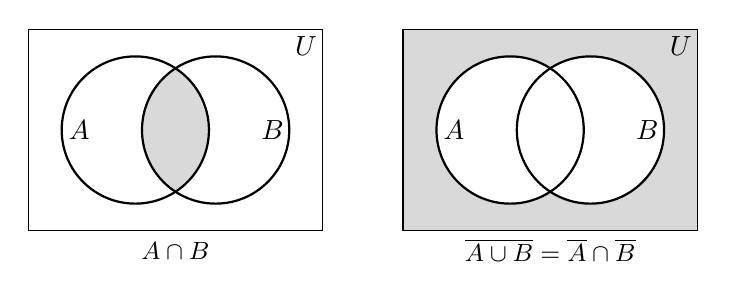
\begin{tikzpicture}[scale=0.85]
  \begin{scope}
    \clip (0,0) circle (1.1cm);
    \fill[gray!30] (1.2,0) circle (1.1cm);
  \end{scope}
  \draw[thick] (0,0) circle (1.1cm) node[left=0.45cm] {$A$};
  \draw[thick] (1.2,0) circle (1.1cm) node[right=0.45cm] {$B$};
  \draw (-1.6,-1.5) rectangle (2.8,1.5); \node at (2.55,1.25) {$U$};
  \node at (0.6,-1.8) {\small $A\cap B$};
  \begin{scope}[xshift=5.6cm]
    \fill[gray!30] (-1.6,-1.5) rectangle (2.8,1.5);
    \fill[white] (0,0) circle (1.1cm);
    \fill[white] (1.2,0) circle (1.1cm);
    \draw[thick] (0,0) circle (1.1cm) node[left=0.45cm] {$A$};
    \draw[thick] (1.2,0) circle (1.1cm) node[right=0.45cm] {$B$};
    \draw (-1.6,-1.5) rectangle (2.8,1.5); \node at (2.55,1.25) {$U$};
    \node at (0.6,-1.8) {\small $\overline{A\cup B}=\overline{A}\cap\overline{B}$};
  \end{scope}
\end{tikzpicture}
\caption{Diagramas de Venn de la intersección y de la primera ley de De Morgan. Un diagrama ilustra una igualdad, pero no la demuestra.}
\label{fig:t1-venn}
\end{figure}

\begin{ejemplo}[Una igualdad por doble inclusión]\label{ej:t1-doble}
Se demuestra que $A\setminus(A\setminus B)=A\cap B$. ($\subseteq$) Si $x\in A\setminus(A\setminus B)$, entonces $x\in A$ y $x\notin A\setminus B$. Como $x\in A$, la única forma de que $x$ no esté en $A\setminus B$ es que $x\in B$; luego $x\in A\cap B$. ($\supseteq$) Si $x\in A\cap B$, entonces $x\in A$ y $x\in B$, luego $x\notin A\setminus B$ y $x\in A\setminus(A\setminus B)$.
\end{ejemplo}

\begin{ejemplo}[Refutar una igualdad]
La afirmación «$(A\cup B)\setminus B=A$ para todos $A$, $B$» es falsa. Un contraejemplo basta: con $A=\{1,2\}$ y $B=\{2\}$, $(A\cup B)\setminus B=\{1\}\neq A$. Lo cierto es $(A\cup B)\setminus B=A\setminus B$.
\end{ejemplo}

\section{Producto cartesiano y familias indexadas}

\begin{definicion}[Producto cartesiano]
Un \emph{par ordenado} $(a,b)$ es un objeto con primera componente $a$ y segunda $b$, con la propiedad $(a,b)=(c,d)\iff a=c\ \text{y}\ b=d$. El \emph{producto cartesiano} de $A$ y $B$ es $A\times B=\{(a,b): a\in A,\ b\in B\}$. Análogamente, $A_1\times\dots\times A_n$ es el conjunto de $n$-tuplas, y $A^{n}=A\times\dots\times A$ ($n$ factores).
\end{definicion}

\begin{proposicion}\label{prop:t1-producto}
Si $A$ y $B$ son finitos, $\abs{A\times B}=\abs{A}\cdot\abs{B}$; en particular, $\abs{A^{n}}=\abs{A}^{n}$. Además, para conjuntos cualesquiera, $A\times(B\cup C)=(A\times B)\cup(A\times C)$.
\end{proposicion}

\begin{proof}
Para cada uno de los $\abs{A}$ valores de la primera componente hay $\abs{B}$ valores posibles de la segunda, y pares distintos se obtienen de elecciones distintas; luego hay $\abs{A}\abs{B}$ pares. La fórmula para $A^{n}$ se sigue por inducción. Para la igualdad: $(a,b)\in A\times(B\cup C)$ si y solo si $a\in A$ y ($b\in B$ o $b\in C$), si y solo si ($a\in A$ y $b\in B$) o ($a\in A$ y $b\in C$), que es la condición de pertenencia a $(A\times B)\cup(A\times C)$.
\end{proof}

\begin{observacion}[Conexión con el curso]
Un vocabulario $\V$ es un conjunto finito, y una secuencia de $T$ tokens es un elemento del producto cartesiano $\V^{T}$; por la \cref{prop:t1-producto}, hay $\abs{\V}^{T}$ secuencias de longitud $T$. El conjunto de todas las secuencias finitas, $\V^{*}=\bigcup_{T\ge 0}\V^{T}$, es la unión de una familia indexada (módulo~1, §1.1). Los conjuntos de candidatos de los métodos de muestreo \emph{top-$k$} y \emph{top-$p$} (módulo~1, tema~4) son subconjuntos de $\V$, y se combinan con intersecciones.
\end{observacion}

\begin{definicion}[Familias indexadas]
Sea $I$ un conjunto de índices y, para cada $i\in I$, un conjunto $A_i$. Se definen
\[
\bigcup_{i\in I}A_i=\{x : x\in A_i\ \text{para algún}\ i\in I\},\qquad
\bigcap_{i\in I}A_i=\{x : x\in A_i\ \text{para todo}\ i\in I\}.
\]
\end{definicion}

\begin{ejemplo}
Sea $A_n=\bigl[0,\tfrac1n\bigr]\subseteq\R$ para $n\ge 1$. Entonces $\bigcup_{n\ge1}A_n=[0,1]$, porque $A_n\subseteq A_1$ para todo $n$, y $\bigcap_{n\ge 1}A_n=\{0\}$: el~0 está en todos, y si $x>0$, eligiendo $n>1/x$ se tiene $x>1/n$, luego $x\notin A_n$. Las leyes de De Morgan se generalizan a familias: $\overline{\bigcup_i A_i}=\bigcap_i\overline{A_i}$ y $\overline{\bigcap_i A_i}=\bigcup_i\overline{A_i}$~\cite[§1.8]{hammack}.
\end{ejemplo}

\begin{observacion}[Errores frecuentes]
(1) Confundir $\in$ con $\subseteq$: $\{1\}\subseteq\{1,2\}$ pero $\{1\}\notin\{1,2\}$. (2) Confundir $\emptyset$ con $\{\emptyset\}$: el primero tiene cero elementos y el segundo uno. (3) Dar un diagrama de Venn o unos cuantos ejemplos como demostración de una igualdad general: la demostración exige tomar un elemento \emph{arbitrario}. (4) Confundir el par ordenado $(a,b)$ con el conjunto $\{a,b\}$: $(1,2)\neq(2,1)$, mientras que $\{1,2\}=\{2,1\}$. (5) Escribir $A\times B=B\times A$: en general es falso.
\end{observacion}

\begin{lecturas}
\item Hammack~\cite{hammack}, cap.~1 «Sets» (§1.1–1.8) y cap.~8 «Proofs Involving Sets» (§8.1–8.3).
\item Velleman~\cite{velleman}, §1.3 «Variables and Sets», §1.4 «Operations on Sets» y §2.3 «More Operations on Sets».
\item Lehman, Leighton y Meyer~\cite{mcs}, §4.1 «Sets».
\item Stanford CS103~\cite{cs103set}, clase «Set Theory Revisited».
\end{lecturas}

\section*{Ejercicios del tema 1}
\addcontentsline{toc}{section}{Ejercicios del tema 1}

\begin{ejercicio}{1}{eje:1-pert}
Sea $A=\{1,\{1\},\{1,2\}\}$. Decida si son verdaderas o falsas: (a) $1\in A$; (b) $\{1\}\in A$; (c) $\{1\}\subseteq A$; (d) $\{2\}\subseteq A$; (e) $\{1,2\}\in A$; (f) $\{\{1,2\}\}\subseteq A$; (g) $\emptyset\subseteq A$; (h) $\emptyset\in A$.
\end{ejercicio}

\begin{ejercicio}{1}{eje:1-card}
Calcule el cardinal de: (a) $\{\emptyset\}$; (b) $\{\emptyset,\{\emptyset\}\}$; (c) $\Pa(\emptyset)$; (d) $\Pa(\Pa(\emptyset))$; (e) $\{\{1,2\},\{2,1\}\}$; (f) $\{1,\{1\},\{\{1\}\}\}$.
\end{ejercicio}

\begin{ejercicio}{2}{eje:1-extension}
Sean $A=\{x\in\Z : x^{2}<10\}$, $B=\{n\in\N : n\ \text{divide a}\ 12,\ n\ge1\}$ y $C=\{x\in\R : x^{2}-3x+2=0\}$. Escriba $A$, $B$ y $C$ por extensión y calcule $A\cap B$, $A\setminus B$, $B\setminus A$, $A\dsim B$ y $(A\cap B)\setminus C$.
\end{ejercicio}

\begin{ejercicio}{2}{eje:1-partes}
Escriba todos los elementos de $\Pa(\{a,b,c\})$. ¿Cuántos contienen a $a$? ¿Cuántos tienen exactamente dos elementos? Generalice: si $\abs{A}=n$ y $a\in A$, ¿cuántos subconjuntos de $A$ contienen a $a$?
\end{ejercicio}

\begin{ejercicio}{2}{eje:1-cartesiano}
Sean $A=\{0,1\}$ y $B=\{\cad{a},\cad{b},\cad{c}\}$. (a) Escriba $A\times B$ por extensión. (b) Calcule $\abs{A^{3}}$ y $\abs{B\times A\times A}$. (c) ¿Es $A\times B=B\times A$? (d) Interprete $A^{8}$ en términos de bytes.
\end{ejercicio}

\begin{ejercicio}{2}{eje:1-demorgan-num}
Sean $U=\{1,2,\dots,10\}$, $A=\{1,2,3,4,5\}$, $B=\{2,4,6,8,10\}$ y $C=\{3,4,5,6\}$. Calcule $\overline{A\cup B}$ y $\overline{A}\cap\overline{B}$, y compruebe la ley de De Morgan. Calcule también $A\setminus(B\cap C)$ y $(A\setminus B)\cup(A\setminus C)$, y explique por qué coinciden.
\end{ejercicio}

\begin{ejercicio}{1}{eje:1-vf}
Decida si son ciertas para todos los conjuntos $A,B,C,D$; si una es falsa, dé un contraejemplo: (a) $(A\cup B)\setminus B=A$; (b) $A\setminus(A\setminus B)=A\cap B$; (c) $(A\times B)\cup(C\times D)=(A\cup C)\times(B\cup D)$.
\end{ejercicio}

\begin{ejercicio}{3}{eje:1-dif-union}
Demuestre que, para conjuntos cualesquiera, $A\setminus(B\cup C)=(A\setminus B)\cap(A\setminus C)$.
\fuente{adaptado de Cambridge, IA Numbers and Sets~\cite{camns}, Example Sheet~1, pregunta~6.}
\end{ejercicio}

\begin{ejercicio}{3}{eje:1-union-inclusion}
Demuestre que $A\subseteq B$ si y solo si $A\cup B=B$. Enuncie y demuestre el resultado análogo para la intersección.
\fuente{adaptado de Stanford CS103~\cite{cs103set}, clase «Set Theory Revisited».}
\end{ejercicio}

\begin{ejercicio}{3}{eje:1-producto-inter}
Demuestre que $A\times(B\cap C)=(A\times B)\cap(A\times C)$ y que $(A\setminus B)\times C=(A\times C)\setminus(B\times C)$.
\fuente{adaptado de Hammack~\cite{hammack}, §8.3 «How to Prove $A=B$», ejercicios de la sección.}
\end{ejercicio}

\begin{ejercicio}{3}{eje:1-simetrica}
(a) Demuestre que $A\dsim B=(A\cup B)\setminus(A\cap B)$. (b) Demuestre que $x\in A\dsim B$ si y solo si $x$ pertenece a exactamente uno de los dos conjuntos. (c) Demuestre que la diferencia simétrica es asociativa: $(A\dsim B)\dsim C=A\dsim(B\dsim C)$.
\fuente{adaptado de Cambridge, IA Numbers and Sets~\cite{camns}, Example Sheet~1, pregunta~13.}
\end{ejercicio}

\begin{ejercicio}{3}{eje:1-partes-inter}
Demuestre que $\Pa(A)\cap\Pa(B)=\Pa(A\cap B)$ y que $\Pa(A)\cup\Pa(B)\subseteq\Pa(A\cup B)$. Muestre con un ejemplo que la segunda inclusión puede ser estricta.
\fuente{adaptado de Hammack~\cite{hammack}, §8.3, ejercicios de la sección.}
\end{ejercicio}

\begin{ejercicio}{3}{eje:1-familias}
(a) Para $n\ge 1$ sea $B_n=\{k\in\N : k\ge n\}$. Demuestre que $B_1\cap\dots\cap B_n\neq\emptyset$ para todo $n$, pero $\bigcap_{n\ge1}B_n=\emptyset$. (b) Calcule $\bigcup_{n\ge1}\bigl(\tfrac1n,2\bigr)$ y $\bigcap_{n\ge1}\bigl(-\tfrac1n,\tfrac1n\bigr)$ y justifique la respuesta.
\fuente{adaptado de Cambridge, IA Numbers and Sets~\cite{camns}, Example Sheet~1, pregunta~7.}
\end{ejercicio}

\begin{ejercicio}{2}{eje:1-cadenas}
Sea $\Sigma=\{\cad{a},\cad{b}\}$ y $\Sigma^{*}$ el conjunto de cadenas sobre $\Sigma$, con $\vacia$ la cadena vacía. Sean $L_1=\{w\in\Sigma^{*}:\abs{w}\le 2\}$ y $L_2=\{w\in\Sigma^{*}: w\ \text{empieza por}\ \cad{a}\}$. (a) Escriba $L_1$ por extensión y calcule $\abs{L_1}$. (b) Escriba $L_1\cap L_2$ y $L_1\setminus L_2$. (c) ¿Es $L_2$ finito?
\end{ejercicio}

% =====================================================================
\chapter{Funciones, imagen y preimagen}
\label{tema:2}
% =====================================================================

Este tema define con precisión qué es una función y estudia cómo actúa sobre subconjuntos mediante la imagen y la preimagen. Sigue las secciones~12.1 y~12.6 de Hammack~\cite{hammack}, las secciones~5.1 y~5.5 de Velleman~\cite{velleman} y la sección~4.3 de~\cite{mcs}. Las propiedades de la imagen y la preimagen son las de la pregunta~9 de la hoja~1 de Cambridge~\cite{camns}.

\section{Definición de función}

\begin{definicion}[Función]\label{def:t2-funcion}
Sean $A$ y $B$ conjuntos. Una \emph{función} $f$ de $A$ en $B$, escrita $f\colon A\to B$, es un subconjunto $f\subseteq A\times B$ tal que para cada $a\in A$ existe \emph{exactamente un} $b\in B$ con $(a,b)\in f$; ese $b$ se denota $f(a)$. El conjunto $A$ es el \emph{dominio} y $B$ el \emph{codominio}. El \emph{recorrido} (o \emph{imagen}) de $f$ es $f(A)=\{f(a): a\in A\}\subseteq B$.
\end{definicion}

La definición contiene dos exigencias: \emph{existencia} (todo elemento del dominio tiene imagen) y \emph{unicidad} (no tiene dos). Dos funciones $f,g\colon A\to B$ son iguales si $f(a)=g(a)$ para todo $a\in A$; la igualdad exige además que el dominio y el codominio coincidan.

\begin{ejemplo}\label{ej:t2-funciones}
\begin{enumerate}
  \item $f\colon\Z\to\Z$, $f(n)=n^{2}$, es una función con recorrido $\{0,1,4,9,\dots\}\subsetneq\Z$.
  \item La \emph{identidad} $\id_A\colon A\to A$, $\id_A(a)=a$.
  \item La \emph{longitud} $\ell\colon\Sigma^{*}\to\N$, $\ell(w)=\abs{w}$, asigna a cada cadena su número de símbolos.
  \item Las \emph{proyecciones} $p_1\colon A\times B\to A$, $p_1(a,b)=a$, y $p_2(a,b)=b$.
  \item La regla «$x\mapsto\sqrt{x}$» \emph{no} define una función $\R\to\R$: falla la existencia, porque $\sqrt{-1}\notin\R$. La regla «$x\mapsto y$ tal que $y^{2}=x$» de $[0,\infty)$ en $\R$ falla la unicidad, porque $4$ tendría las imágenes $2$ y $-2$.
\end{enumerate}
\end{ejemplo}

\begin{ejemplo}[Funciones bien definidas]\label{ej:t2-biendef}
Cuando los elementos del dominio admiten varias representaciones, hay que comprobar que la regla no depende de la representación elegida. La regla $f\bigl(\tfrac{a}{b}\bigr)=a+b$ no define una función $\Q\to\Z$: $\tfrac12=\tfrac24$, pero $1+2=3\neq 6=2+4$. En cambio, $g\bigl(\tfrac ab\bigr)=\tfrac{2a}{b}$ sí está bien definida: si $\tfrac ab=\tfrac cd$, entonces $\tfrac{2a}{b}=2\cdot\tfrac ab=2\cdot\tfrac cd=\tfrac{2c}{d}$.
\end{ejemplo}

\section{El conjunto de funciones}

\begin{definicion}
$B^{A}$ denota el conjunto de todas las funciones $A\to B$.
\end{definicion}

\begin{proposicion}\label{prop:t2-contar}
Si $A$ y $B$ son finitos, $\abs{B^{A}}=\abs{B}^{\abs{A}}$.
\end{proposicion}

\begin{proof}
Sea $A=\{a_1,\dots,a_m\}$. Una función $f\colon A\to B$ queda determinada por la lista de valores $(f(a_1),\dots,f(a_m))\in B^{m}$, y toda lista de $B^{m}$ define una función. Luego $\abs{B^{A}}=\abs{B^{m}}=\abs{B}^{m}$ por la \cref{prop:t1-producto}.
\end{proof}

\begin{definicion}[Función característica]
Sea $X\subseteq U$. La \emph{función característica} (o \emph{indicadora}) de $X$ es $\chi_X\colon U\to\{0,1\}$, con $\chi_X(u)=1$ si $u\in X$ y $\chi_X(u)=0$ si $u\notin X$.
\end{definicion}

Cada subconjunto de $U$ determina su función característica y cada función $U\to\{0,1\}$ es la característica de un único subconjunto, el de los elementos que van al~1. Con $\abs{U}=n$, la \cref{prop:t2-contar} da $\abs{\{0,1\}^{U}}=2^{n}$, de nuevo el \cref{teo:t1-partes}. En el \cref{tema:3} se formaliza esta correspondencia como una biyección.

\section{Imagen y preimagen de subconjuntos}

\begin{definicion}[Imagen y preimagen]\label{def:t2-imagen}
Sea $f\colon A\to B$. Para $X\subseteq A$ y $Y\subseteq B$ se definen la \emph{imagen} de $X$ y la \emph{preimagen} (o \emph{imagen inversa}) de $Y$:
\[
f(X)=\{f(x): x\in X\}\subseteq B,\qquad f^{-1}(Y)=\{a\in A: f(a)\in Y\}\subseteq A.
\]
\end{definicion}

La notación $f^{-1}(Y)$ tiene sentido para \emph{cualquier} función, sea o no invertible: es un conjunto, no la aplicación de una función inversa. Si $Y=\{b\}$, el conjunto $f^{-1}(\{b\})$ se llama \emph{fibra} de $b$.

\begin{ejemplo}\label{ej:t2-cuadrado}
Sea $f\colon\R\to\R$, $f(x)=x^{2}$. Entonces $f([-1,2])=[0,4]$, porque $x^{2}$ recorre $[0,1]$ en $[-1,0]$ y $[0,4]$ en $[0,2]$. Además, $f^{-1}([1,4])=[-2,-1]\cup[1,2]$, $f^{-1}(\{-1\})=\emptyset$ y $f^{-1}(f([0,1]))=f^{-1}([0,1])=[-1,1]\supsetneq[0,1]$.
\end{ejemplo}

\begin{teorema}[Propiedades de la preimagen]\label{teo:t2-preimagen}
Sea $f\colon A\to B$ y sean $C,D\subseteq B$. Entonces
\begin{gather*}
f^{-1}(C\cup D)=f^{-1}(C)\cup f^{-1}(D),\qquad f^{-1}(C\cap D)=f^{-1}(C)\cap f^{-1}(D),\\
f^{-1}(B\setminus C)=A\setminus f^{-1}(C).
\end{gather*}
\end{teorema}

\begin{proof}
Se demuestra la primera; las otras dos se dejan como ejercicio (\cref{eje:2-preim-ui,eje:2-preim-comp}). Para todo $a\in A$:
$a\in f^{-1}(C\cup D)\iff f(a)\in C\cup D\iff f(a)\in C\ \text{o}\ f(a)\in D\iff a\in f^{-1}(C)\ \text{o}\ a\in f^{-1}(D)\iff a\in f^{-1}(C)\cup f^{-1}(D)$.
\end{proof}

\begin{teorema}[Propiedades de la imagen]\label{teo:t2-imagen}
Sea $f\colon A\to B$, $X_1,X_2,X\subseteq A$ e $Y\subseteq B$. Entonces
\begin{enumerate}
  \item $f(X_1\cup X_2)=f(X_1)\cup f(X_2)$;
  \item $f(X_1\cap X_2)\subseteq f(X_1)\cap f(X_2)$, y la inclusión puede ser estricta;
  \item $X\subseteq f^{-1}(f(X))$ y $f(f^{-1}(Y))\subseteq Y$.
\end{enumerate}
\end{teorema}

\begin{proof}
(ii) Si $b\in f(X_1\cap X_2)$, existe $x\in X_1\cap X_2$ con $f(x)=b$; como $x\in X_1$, $b\in f(X_1)$, y como $x\in X_2$, $b\in f(X_2)$. Para la desigualdad estricta, sea $f(x)=x^{2}$, $X_1=\{-1\}$ y $X_2=\{1\}$: $f(X_1\cap X_2)=f(\emptyset)=\emptyset$, mientras que $f(X_1)\cap f(X_2)=\{1\}$. Los apartados (i) y~(iii) son los \cref{eje:2-imagen-ui,eje:2-ida-vuelta}.
\end{proof}

La asimetría entre ambos teoremas es instructiva: la preimagen respeta todas las operaciones de conjuntos, mientras que la imagen solo respeta la unión. La razón es que la imagen puede «pegar» elementos distintos; en el \cref{tema:3} se verá que las igualdades $f(X_1\cap X_2)=f(X_1)\cap f(X_2)$ y $f^{-1}(f(X))=X$ son ciertas exactamente cuando $f$ es inyectiva.

\section{Otras construcciones}

Una \emph{sucesión} de elementos de $A$ es una función $\N\to A$, $n\mapsto a_n$. Una \emph{cadena} de longitud $n$ sobre $\Sigma$ puede verse como una función $\{1,\dots,n\}\to\Sigma$ que asigna a cada posición su símbolo. Si $f\colon A\to B$ y $X\subseteq A$, la \emph{restricción} $f|_X\colon X\to B$ es la función $f|_X(x)=f(x)$. Las funciones \emph{definidas a trozos} asignan reglas distintas a partes disjuntas del dominio que lo recubren.

\begin{observacion}[Conexión con el curso]
Un modelo de lenguaje es una función $P\colon\V^{*}\to[0,1]$ (módulo~1, §1.3), y una matriz de \emph{embeddings} define una función $E\colon\V\to\R^{d}$ (módulo~12, tema~4). La preimagen aparece de forma natural: para la longitud $\ell\colon\V^{*}\to\N$, la fibra $\ell^{-1}(\{T\})$ es $\V^{T}$; para la función que elige el token de mayor logit (decodificación voraz, módulo~1, tema~4), la preimagen de un token es la región del espacio de logits en la que ese token gana.
\end{observacion}

\begin{observacion}[Errores frecuentes]
(1) Confundir codominio y recorrido: $f(x)=x^{2}$ de $\R$ en $\R$ tiene codominio $\R$ y recorrido $[0,\infty)$. (2) Leer $f^{-1}(Y)$ como «aplicar la inversa»: la preimagen existe siempre, la inversa solo para biyecciones. (3) Olvidar comprobar que una regla está bien definida cuando el dominio tiene representaciones múltiples (fracciones, clases de equivalencia). (4) Suponer que $f^{-1}(f(X))=X$: solo se tiene la inclusión $\supseteq$ en general.
\end{observacion}

\begin{lecturas}
\item Hammack~\cite{hammack}, §12.1 «Functions» y §12.6 «Image and Preimage».
\item Velleman~\cite{velleman}, §5.1 «Functions» y §5.5 «Images and Inverse Images: A Research Project».
\item Lehman, Leighton y Meyer~\cite{mcs}, §4.3 «Functions».
\end{lecturas}

\section*{Ejercicios del tema 2}
\addcontentsline{toc}{section}{Ejercicios del tema 2}

\begin{ejercicio}{1}{eje:2-esfuncion}
Decida si cada una de las siguientes es una función y, si no lo es, qué exigencia falla. (a) $R_1=\{(1,\cad{a}),(2,\cad{a}),(3,\cad{b})\}\subseteq\{1,2,3\}\times\{\cad{a},\cad{b}\}$. (b) $R_2=\{(1,\cad{a}),(2,\cad{b})\}$, con los mismos conjuntos. (c) $R_3=\{(1,\cad{a}),(1,\cad{b}),(2,\cad{a}),(3,\cad{a})\}$. (d) $x\mapsto 1/x$ de $\R$ en $\R$. (e) $\tfrac ab\mapsto\tfrac{a+1}{b+1}$ de $\Q_{>0}$ en $\Q$, con $a,b\in\N$, $a,b\ge1$.
\end{ejercicio}

\begin{ejercicio}{2}{eje:2-tabla}
Sean $A=\{0,1,2,3,4\}$, $B=\{1,2,3,4,5\}$ y
\[
f=\{(0,2),(1,4),(2,2),(3,1),(4,2)\}.
\]
(a) Compruebe que $f$ es una función $A\to B$ y dé su dominio, codominio y recorrido. (b) Calcule $f(\{0,1,2\})$, $f^{-1}(\{2\})$, $f^{-1}(\{3,5\})$ y $f^{-1}(\{1,4\})$.
\fuente{adaptado de Hammack~\cite{hammack}, §12.1 «Functions», ejercicios de la sección (datos cambiados).}
\end{ejercicio}

\begin{ejercicio}{2}{eje:2-contar}
(a) ¿Cuántas funciones hay de un conjunto de 3 elementos en uno de 4? ¿Y de uno de 4 en uno de 3? (b) ¿Cuántas funciones $\{0,1\}^{2}\to\{0,1\}$ (funciones booleanas de dos variables) existen? (c) ¿Cuántas funciones $\{0,1\}^{n}\to\{0,1\}$? Evalúe para $n=3$.
\end{ejercicio}

\begin{ejercicio}{2}{eje:2-cuadrado}
Sea $f\colon\R\to\R$, $f(x)=x^{2}-2x$. Calcule $f([0,3])$, $f^{-1}(\{3\})$, $f^{-1}([-1,0])$, $f^{-1}((-\infty,-2))$ y $f^{-1}(f(\{3\}))$.
\fuente{adaptado de Hammack~\cite{hammack}, §12.6 «Image and Preimage», ejercicios de la sección.}
\end{ejercicio}

\begin{ejercicio}{2}{eje:2-suelo}
Sea $f\colon\Z\to\Z$, $f(n)=\lfloor n/2\rfloor$. Calcule $f(\{0,1,2,3\})$, $f^{-1}(\{1\})$, $f^{-1}(\{0,1,2\})$ y $f(2\Z)$, donde $2\Z$ es el conjunto de los enteros pares. ¿Cuál es el recorrido de $f$?
\end{ejercicio}

\begin{ejercicio}{2}{eje:2-longitud}
Sea $\Sigma=\{\cad{a},\cad{b}\}$ y $\ell\colon\Sigma^{*}\to\N$ la longitud. Calcule $\ell^{-1}(\{2\})$, $\ell^{-1}(\{0,1\})$, $\ell(\{\cad{ab},\cad{ba},\cad{aab}\})$ y el recorrido de $\ell$. ¿Cuántos elementos tiene $\ell^{-1}(\{n\})$?
\end{ejercicio}

\begin{ejercicio}{1}{eje:2-recorrido}
Dé el recorrido de cada función $\R\to\R$: (a) $f(x)=e^{x}$; (b) $g(x)=\operatorname{sen}x$; (c) $h(x)=x^{2}+2x+3$; (d) $k(x)=\dfrac{1}{1+x^{2}}$.
\end{ejercicio}

\begin{ejercicio}{3}{eje:2-preim-ui}
Sea $f\colon X\to Y$ y $C,D\subseteq Y$. Demuestre que $f^{-1}(C\cap D)=f^{-1}(C)\cap f^{-1}(D)$ y que, si $C\subseteq D$, entonces $f^{-1}(C)\subseteq f^{-1}(D)$.
\fuente{adaptado de Cambridge, IA Numbers and Sets~\cite{camns}, Example Sheet~1, pregunta~9.}
\end{ejercicio}

\begin{ejercicio}{3}{eje:2-imagen-ui}
Sea $f\colon X\to Y$ y $A,B\subseteq X$. Demuestre que $f(A\cup B)=f(A)\cup f(B)$. Decida si $f(A\setminus B)=f(A)\setminus f(B)$ es siempre cierta; si no, dé un contraejemplo y la inclusión que sí se cumple.
\fuente{adaptado de Cambridge, IA Numbers and Sets~\cite{camns}, Example Sheet~1, pregunta~9.}
\end{ejercicio}

\begin{ejercicio}{3}{eje:2-ida-vuelta}
Sea $f\colon X\to Y$, $A\subseteq X$ y $C\subseteq Y$. Demuestre que $A\subseteq f^{-1}(f(A))$ y que $f(f^{-1}(C))\subseteq C$. Dé ejemplos en los que ambas inclusiones son estrictas.
\fuente{adaptado de Cambridge, IA Numbers and Sets~\cite{camns}, Example Sheet~1, pregunta~9.}
\end{ejercicio}

\begin{ejercicio}{3}{eje:2-preim-comp}
Sea $f\colon X\to Y$ y $C\subseteq Y$. Demuestre que $f^{-1}(Y\setminus C)=X\setminus f^{-1}(C)$, que $f^{-1}(\emptyset)=\emptyset$ y que $f^{-1}(Y)=X$.
\fuente{adaptado de Cambridge, Discrete Mathematics~\cite{camdm}, hoja~8, ejercicio~12.2.5.}
\end{ejercicio}

\begin{ejercicio}{2}{eje:2-caracteristica}
Sean $X,Z\subseteq U$. Compruebe, distinguiendo casos según la pertenencia de $u$ a $X$ y a $Z$, que para todo $u\in U$:
$\chi_{X\cap Z}(u)=\chi_X(u)\chi_Z(u)$, \ $\chi_{X\cup Z}(u)=\chi_X(u)+\chi_Z(u)-\chi_X(u)\chi_Z(u)$ \ y \ $\chi_{\overline{X}}(u)=1-\chi_X(u)$.
Deduzca que, si $U$ es finito, $\abs{X\cup Z}=\abs{X}+\abs{Z}-\abs{X\cap Z}$.
\end{ejercicio}

\begin{ejercicio}{3}{eje:2-biendef}
Decida si las reglas siguientes definen funciones $\Q\to\Q$ y demuéstrelo: (a) $f\bigl(\tfrac ab\bigr)=\tfrac{a^{2}}{b^{2}}$; (b) $g\bigl(\tfrac ab\bigr)=\tfrac{a+b}{b}$; (c) $h\bigl(\tfrac ab\bigr)=\tfrac{a}{b+1}$ (con $b\ge1$). En todos los casos $a\in\Z$ y $b\in\Z$, $b\neq0$.
\end{ejercicio}

\begin{ejercicio}{2}{eje:2-argmax}
Sea $g\colon\R^{3}\to\{1,2,3\}$ la función que devuelve el índice de la mayor coordenada y, en caso de empate, el menor de los índices empatados (decodificación voraz). (a) Calcule $g(1,3,2)$, $g(2,2,1)$ y $g(0,0,0)$. (b) Describa $g^{-1}(\{1\})$ y $g^{-1}(\{3\})$ mediante desigualdades. (c) ¿Es $g^{-1}(\{1\})\cup g^{-1}(\{2\})\cup g^{-1}(\{3\})=\R^{3}$? ¿Son disjuntas las tres fibras?
\end{ejercicio}

% =====================================================================
\chapter{Funciones inyectivas, sobreyectivas y biyectivas}
\label{tema:3}
% =====================================================================

Este tema es el núcleo práctico del módulo: decidir si una función es inyectiva, sobreyectiva o biyectiva y \emph{demostrarlo}. Sigue la sección~12.2 de Hammack~\cite{hammack}, la sección~5.2 de Velleman~\cite{velleman} y las secciones~4.3 y~4.5 de~\cite{mcs}. Los ejercicios de clasificación siguen el problema~1 de la hoja~3 de Stanford CS103~\cite{cs103ps3}.

\section{Definiciones y método de demostración}

\begin{definicion}\label{def:t3-iny}
Sea $f\colon A\to B$.
\begin{enumerate}
  \item $f$ es \emph{inyectiva} si elementos distintos tienen imágenes distintas: para todos $a,a'\in A$, si $f(a)=f(a')$ entonces $a=a'$.
  \item $f$ es \emph{sobreyectiva} si todo elemento del codominio es imagen de alguno: para todo $b\in B$ existe $a\in A$ con $f(a)=b$; equivalentemente, $f(A)=B$.
  \item $f$ es \emph{biyectiva} si es inyectiva y sobreyectiva.
\end{enumerate}
\end{definicion}

En términos de fibras: $f$ es inyectiva si cada fibra $f^{-1}(\{b\})$ tiene \emph{a lo sumo} un elemento, sobreyectiva si tiene \emph{al menos} uno y biyectiva si tiene \emph{exactamente} uno. La \cref{fig:t3-flechas} muestra los cuatro casos posibles con diagramas de flechas.

\begin{figure}[h]
\centering
\begin{tikzpicture}[>={Stealth[length=1.6mm]},font=\small,
  pt/.style={circle,fill,inner sep=1.2pt}]
  \foreach \col/\tit/\na/\nb/\arr in {
    0/{inyectiva,\\ no sobreyectiva}/2/3/{1/1,2/3},
    3.4/{sobreyectiva,\\ no inyectiva}/3/2/{1/1,2/1,3/2},
    6.8/{biyectiva}/3/3/{1/2,2/3,3/1},
    10.2/{ninguna}/3/3/{1/1,2/1,3/3}} {
    \begin{scope}[xshift=\col cm]
      \foreach \i in {1,...,\na} \node[pt] (a\i) at (0,-0.6*\i) {};
      \foreach \j in {1,...,\nb} \node[pt] (b\j) at (1.4,-0.6*\j) {};
      \draw[rounded corners] (-0.3,-0.25) rectangle (0.3,-0.6*\na-0.35);
      \draw[rounded corners] (1.1,-0.25) rectangle (1.7,-0.6*\nb-0.35);
      \foreach \u/\v in \arr \draw[->] (a\u) -- (b\v);
      \node[align=center,anchor=north] at (0.7,-2.3) {\tit};
    \end{scope}}
\end{tikzpicture}
\caption{Diagramas de flechas de funciones entre conjuntos finitos.}
\label{fig:t3-flechas}
\end{figure}

\paragraph{Cómo demostrar cada propiedad.}
\begin{itemize}[leftmargin=1.4em]
  \item \emph{Inyectividad}: se supone $f(a)=f(a')$ para $a,a'$ arbitrarios y se deduce $a=a'$ (demostración directa), o se supone $a\neq a'$ y se deduce $f(a)\neq f(a')$ (contrarrecíproco).
  \item \emph{No inyectividad}: basta un contraejemplo, $a\neq a'$ con $f(a)=f(a')$.
  \item \emph{Sobreyectividad}: se toma $b\in B$ arbitrario, se \emph{busca} un candidato $a$ (normalmente resolviendo la ecuación $f(a)=b$ en borrador), y se \emph{comprueba} que $a\in A$ y que $f(a)=b$.
  \item \emph{No sobreyectividad}: basta un $b\in B$ y una prueba de que la ecuación $f(a)=b$ no tiene solución en $A$.
\end{itemize}

\begin{ejemplo}\label{ej:t3-2n1}
Sea $f\colon\Z\to\Z$, $f(n)=2n+1$. \emph{Es inyectiva}: si $2n+1=2m+1$, restando~1 y dividiendo entre~2 se obtiene $n=m$. \emph{No es sobreyectiva}: $f(n)$ es siempre impar, luego $2$ no tiene preimagen. En cambio, $g\colon\R\to\R$, $g(x)=2x+1$, es biyectiva: la inyectividad se prueba igual y, dado $y\in\R$, el número $x=(y-1)/2$ es real y cumple $g(x)=y$. El mismo cálculo falla en $\Z$ porque $(y-1)/2$ no es entero cuando $y$ es par: la sobreyectividad depende del dominio.
\end{ejemplo}

\begin{ejemplo}[Dominio y codominio importan]\label{ej:t3-cuadrado}
La regla $x\mapsto x^{2}$ da cuatro funciones distintas:
\begin{center}\small
\begin{tabular}{@{}lccl@{}}
\toprule
Función & Inyectiva & Sobreyectiva & Motivo \\
\midrule
$\R\to\R$ & no & no & $f(-1)=f(1)$; $-1$ no tiene preimagen \\
$\R\to[0,\infty)$ & no & sí & $f(-1)=f(1)$; $y\ge0$ es $f(\sqrt y)$ \\
$[0,\infty)\to\R$ & sí & no & $x^{2}=x'^{2}$ con $x,x'\ge0$ da $x=x'$ \\
$[0,\infty)\to[0,\infty)$ & sí & sí & las dos razones anteriores \\
\bottomrule
\end{tabular}
\end{center}
\end{ejemplo}

\begin{ejemplo}[Una función de dos variables]\label{ej:t3-suma}
Sea $s\colon\Z\times\Z\to\Z$, $s(m,n)=m+n$. Es sobreyectiva, pues $s(k,0)=k$ para todo $k\in\Z$, y no es inyectiva, pues $s(1,0)=s(0,1)$ con $(1,0)\neq(0,1)$.
\end{ejemplo}

\begin{ejemplo}[Funciones sobre cadenas]\label{ej:t3-cadenas}
Sea $\Sigma$ un alfabeto. La función $c\colon\Sigma^{*}\to\Sigma^{*}$, $c(w)=\cad{a}w$ (anteponer el símbolo $\cad{a}\in\Sigma$), es inyectiva: si $\cad{a}w=\cad{a}w'$, al suprimir el primer símbolo de ambas cadenas queda $w=w'$. No es sobreyectiva: la cadena vacía $\vacia$ no empieza por $\cad{a}$. La longitud $\ell\colon\Sigma^{*}\to\N$ es sobreyectiva si $\Sigma\neq\emptyset$ (la cadena $\cad{a}^{n}$ tiene longitud $n$) y no es inyectiva si $\abs{\Sigma}\ge2$.
\end{ejemplo}

\section{Criterios para funciones reales}

\begin{definicion}
$f\colon A\to\R$, con $A\subseteq\R$, es \emph{estrictamente creciente} si $x<x'$ implica $f(x)<f(x')$, y \emph{estrictamente decreciente} si $x<x'$ implica $f(x)>f(x')$. Es \emph{estrictamente monótona} si es una de las dos.
\end{definicion}

\begin{proposicion}\label{prop:t3-monotona}
Toda función estrictamente monótona es inyectiva.
\end{proposicion}

\begin{proof}
Sea $f$ estrictamente creciente y sean $x\neq x'$. Sin pérdida de generalidad, $x<x'$; entonces $f(x)<f(x')$, luego $f(x)\neq f(x')$. El caso decreciente es igual.
\end{proof}

Si $f$ es derivable en un intervalo con $f'>0$ en todo punto, entonces es estrictamente creciente (consecuencia del teorema del valor medio, que se estudia en el módulo de cálculo de esta fase), y por tanto inyectiva. Para la sobreyectividad sobre un intervalo, el teorema de Bolzano (valores intermedios) permite concluir que una función continua toma todos los valores comprendidos entre sus límites; en este módulo se prefiere resolver $f(x)=y$ explícitamente.

\begin{ejemplo}[La sigmoide]\label{ej:t3-sigmoide}
Sea $\sigma\colon\R\to(0,1)$, $\sigma(x)=1/(1+e^{-x})$. Es inyectiva: si $\sigma(x)=\sigma(x')$, entonces $1+e^{-x}=1+e^{-x'}$, luego $e^{-x}=e^{-x'}$ y, por la inyectividad de la exponencial, $x=x'$. Es sobreyectiva sobre $(0,1)$: dado $y\in(0,1)$, se resuelve $1+e^{-x}=1/y$, es decir, $e^{-x}=(1-y)/y>0$, y $x=\ln\bigl(y/(1-y)\bigr)$ es un número real que cumple $\sigma(x)=y$. La sigmoide es la función de activación del módulo~11 y su inversa es el \emph{logit}.
\end{ejemplo}

\section{Funciones entre conjuntos finitos}

\begin{proposicion}\label{prop:t3-finitos}
Sean $A$ y $B$ finitos y $f\colon A\to B$.
\begin{enumerate}
  \item Si $f$ es inyectiva, $\abs{A}\le\abs{B}$; si es sobreyectiva, $\abs{A}\ge\abs{B}$.
  \item Si $\abs{A}=\abs{B}$, entonces $f$ es inyectiva si y solo si es sobreyectiva.
\end{enumerate}
\end{proposicion}

\begin{proof}
(i) El dominio es la unión disjunta de las fibras: $\abs{A}=\sum_{b\in B}\abs{f^{-1}(\{b\})}$. Si $f$ es inyectiva, cada sumando es $\le1$ y la suma es $\le\abs{B}$; si es sobreyectiva, cada sumando es $\ge1$ y la suma es $\ge\abs{B}$. (ii) Si $f$ es inyectiva, las fibras tienen a lo sumo un elemento y $\abs{f(A)}=\abs{A}=\abs{B}$; como $f(A)\subseteq B$ y ambos son finitos con el mismo cardinal, $f(A)=B$. El recíproco es el \cref{eje:3-finitos}.
\end{proof}

\begin{proposicion}\label{prop:t3-contar-iny}
Si $\abs{A}=k$ y $\abs{B}=n$, el número de funciones inyectivas $A\to B$ es $n(n-1)\cdots(n-k+1)$, que vale~0 si $k>n$. En particular, hay $n!$ biyecciones entre dos conjuntos de $n$ elementos.
\end{proposicion}

\begin{proof}
Sea $A=\{a_1,\dots,a_k\}$. Para $f(a_1)$ hay $n$ elecciones; para $f(a_2)$, $n-1$ (debe ser distinto del anterior); y así hasta $f(a_k)$, con $n-k+1$ elecciones. Si $k>n$ alguno de los factores es cero.
\end{proof}

\begin{observacion}[Conexión con el curso]
Un tokenizador debe ser \emph{inyectivo}: dos textos distintos no pueden producir la misma secuencia de tokens, o el texto original no podría recuperarse (módulo~1, §1.2). La codificación UTF-8 es inyectiva y ningún código es prefijo de otro, lo que garantiza que una cadena de bytes se descompone de una sola manera (módulo~12, §1.4). La asignación de índices a los tokens, $\V\to\{0,\dots,K-1\}$, es una biyección. En cambio, la decodificación de tokens a texto \emph{no} es inyectiva en general: las secuencias $(\cad{a},\cad{b})$ y $(\cad{ab})$ producen el mismo texto (\cref{eje:3-codigos}).
\end{observacion}

\begin{observacion}[Errores frecuentes]
(1) «Demostrar» la inyectividad partiendo de $a=a'$ y llegando a $f(a)=f(a')$: eso prueba solo que $f$ está bien definida. (2) Comprobar unos cuantos valores en lugar de razonar con elementos arbitrarios. (3) En la sobreyectividad, no comprobar que el candidato pertenece al dominio: $(y-1)/2$ resuelve $2n+1=y$ pero no es entero si $y$ es par. (4) Olvidar que inyectividad y sobreyectividad dependen del dominio y del codominio, no solo de la fórmula (\cref{ej:t3-cuadrado}).
\end{observacion}

\begin{lecturas}
\item Hammack~\cite{hammack}, §12.2 «Injective and Surjective Functions».
\item Velleman~\cite{velleman}, §5.2 «One-to-One and Onto».
\item Lehman, Leighton y Meyer~\cite{mcs}, §4.3 «Functions» y §4.5 «Finite Cardinality».
\item Stanford CS103~\cite{cs103ps3}, Problem Set~3, problemas 1 a~3.
\end{lecturas}

\section*{Ejercicios del tema 3}
\addcontentsline{toc}{section}{Ejercicios del tema 3}

\begin{ejercicio}{1}{eje:3-tablas}
Clasifique (inyectiva, sobreyectiva, biyectiva o ninguna) las funciones $\{1,2,3\}\to\{\cad{a},\cad{b},\cad{c}\}$ dadas por: (a) $1\mapsto\cad{a}$, $2\mapsto\cad{b}$, $3\mapsto\cad{c}$; (b) $1\mapsto\cad{a}$, $2\mapsto\cad{a}$, $3\mapsto\cad{c}$; (c) $1\mapsto\cad{c}$, $2\mapsto\cad{a}$, $3\mapsto\cad{b}$; (d) $1\mapsto\cad{b}$, $2\mapsto\cad{b}$, $3\mapsto\cad{b}$. Para las que no sean biyectivas, ¿podría ser alguna inyectiva sin ser sobreyectiva?
\end{ejercicio}

\begin{ejercicio}{1}{eje:3-error}
Se propone la siguiente «demostración» de que $f\colon\Z\to\Z$, $f(n)=n^{2}$, es inyectiva: «Sean $a,b\in\Z$ con $a=b$. Entonces $a^{2}=b^{2}$, es decir, $f(a)=f(b)$. Luego $f$ es inyectiva.» Señale el error y decida si $f$ es inyectiva.
\end{ejercicio}

\begin{ejercicio}{2}{eje:3-clasificar}
Clasifique, justificando brevemente: (a) $\Z\to\Z$, $n\mapsto n+3$; (b) $\Z\to\Z$, $n\mapsto 2n$; (c) $\Z\to\Z$, $n\mapsto n^{3}$; (d) $\N\to\N$, $n\mapsto n+1$; (e) $\R\to\R$, $x\mapsto x^{3}-x$; (f) $\R\to\R$, $x\mapsto e^{x}$; (g) $\R\to\Z$, $x\mapsto\lfloor x\rfloor$; (h) $\Z\to\N$, $n\mapsto\abs{n}$.
\fuente{adaptado de Stanford CS103~\cite{cs103ps3}, Problem Set~3, problema~1 «Properties of Functions».}
\end{ejercicio}

\begin{ejercicio}{2}{eje:3-5n2}
Sea $f\colon\Z\to\Z$, $f(n)=5n+2$. Demuestre que $f$ es inyectiva y no sobreyectiva. ¿Qué ocurre con la misma fórmula como función $\Q\to\Q$?
\fuente{adaptado de Hammack~\cite{hammack}, §12.2, ejercicios de la sección.}
\end{ejercicio}

\begin{ejercicio}{2}{eje:3-homografica}
Sea $f\colon\R\setminus\{2\}\to\R\setminus\{3\}$, $f(x)=\dfrac{3x+1}{x-2}$. (a) Compruebe que $f(x)\neq3$ para todo $x$ del dominio, de modo que el codominio es correcto. (b) Demuestre que $f$ es biyectiva y obtenga la expresión de la única preimagen de cada $y$.
\fuente{adaptado de University of Washington, Math 300~\cite{uw300}, «Problems on functions», problema~5.}
\end{ejercicio}

\begin{ejercicio}{3}{eje:3-lineal-z2}
Sea $f\colon\Z\times\Z\to\Z\times\Z$, $f(m,n)=(m+n,\ m+2n)$. Demuestre que $f$ es biyectiva.
\fuente{adaptado de Hammack~\cite{hammack}, §12.2, ejercicios de la sección.}
\end{ejercicio}

\begin{ejercicio}{3}{eje:3-2m3n}
Sea $f\colon\Z\times\Z\to\Z$, $f(m,n)=2m+3n$. Demuestre que $f$ es sobreyectiva y no inyectiva. ¿Es sobreyectiva $g(m,n)=2m+4n$?
\fuente{adaptado de Hammack~\cite{hammack}, §12.2, ejercicios de la sección.}
\end{ejercicio}

\begin{ejercicio}{3}{eje:3-NZ}
Sea $f\colon\N\to\Z$ definida por $f(n)=n/2$ si $n$ es par y $f(n)=-(n+1)/2$ si $n$ es impar. (a) Calcule $f(0),\dots,f(6)$. (b) Demuestre que $f$ es biyectiva.
\fuente{adaptado de Stanford CS103~\cite{cs103ps3}, Problem Set~3, problema~2.}
\end{ejercicio}

\begin{ejercicio}{3}{eje:3-creciente}
(a) Decida si $x\mapsto x^{2}$ y $x\mapsto x^{3}$ son estrictamente crecientes en $\R$. (b) Demuestre que si $f,g\colon\R\to\R$ son estrictamente crecientes, también lo es $g\circ f$ (la composición se define en el \cref{tema:4}: $(g\circ f)(x)=g(f(x))$). (c) ¿Es cierto que toda función inyectiva $\R\to\R$ es estrictamente monótona? Demuéstrelo o dé un contraejemplo.
\fuente{adaptado de Stanford CS103~\cite{cs103ps3}, Problem Set~3, problema~3 «Strictly Increasing Functions».}
\end{ejercicio}

\begin{ejercicio}{3}{eje:3-cadenas}
Sea $\Sigma=\{\cad{a},\cad{b}\}$. Para cada función $\Sigma^{*}\to\Sigma^{*}$, decida si es inyectiva y si es sobreyectiva, y demuéstrelo: (a) la inversión $r(w_1w_2\cdots w_n)=w_n\cdots w_2w_1$; (b) la duplicación $d(w)=ww$; (c) la función $q$ que suprime el último símbolo de una cadena no vacía y deja igual la cadena vacía.
\end{ejercicio}

\begin{ejercicio}{3}{eje:3-codigos}
Sea $\Sigma$ un alfabeto finito, $k\ge1$ y $c\colon\Sigma\to\{0,1\}^{k}$ una función inyectiva (un \emph{código de longitud fija}). Su extensión $c^{*}\colon\Sigma^{*}\to\{0,1\}^{*}$ concatena los códigos: $c^{*}(x_1\cdots x_n)=c(x_1)\cdots c(x_n)$. (a) Demuestre que $c^{*}$ es inyectiva. (b) Sea ahora el código de longitud variable $c(\cad{x})=0$, $c(\cad{y})=01$, $c(\cad{z})=1$. Demuestre que $c$ es inyectiva pero $c^{*}$ no lo es. (c) Relacione (b) con la decodificación de un vocabulario que contiene \cad{a}, \cad{b} y \cad{ab}.
\end{ejercicio}

\begin{ejercicio}{2}{eje:3-contar}
Calcule el número de funciones, de funciones inyectivas, de sobreyectivas y de biyectivas: (a) de $\{1,2,3\}$ en $\{1,2,3,4\}$; (b) de $\{1,2,3,4\}$ en $\{1,2,3\}$; (c) de $\{1,2,3\}$ en sí mismo. Para el número de sobreyecciones de~(b), razone qué elemento de la imagen tiene dos preimágenes.
\end{ejercicio}

\begin{ejercicio}{3}{eje:3-finitos}
Sean $A$ y $B$ conjuntos finitos con $\abs{A}=\abs{B}$ y $f\colon A\to B$ sobreyectiva. Demuestre que $f$ es inyectiva. Muestre con un ejemplo que el resultado es falso para conjuntos infinitos.
\fuente{adaptado de Lehman, Leighton y Meyer~\cite{mcs}, §4.5 «Finite Cardinality».}
\end{ejercicio}

\begin{ejercicio}{3}{eje:3-softsign}
Sea $f\colon\R\to(-1,1)$, $f(x)=\dfrac{x}{1+\abs{x}}$. (a) Compruebe que $f(x)\in(-1,1)$ para todo $x$. (b) Demuestre que $f$ es inyectiva. (c) Demuestre que es sobreyectiva y halle la preimagen de cada $y\in(-1,1)$.
\end{ejercicio}

\begin{ejercicio}{2}{eje:3-tanh}
Sea $\tanh\colon\R\to(-1,1)$, $\tanh x=\dfrac{e^{x}-e^{-x}}{e^{x}+e^{-x}}$. Demuestre que es biyectiva resolviendo $\tanh x=y$ y compruebe que la preimagen de $y$ es $\tfrac12\ln\dfrac{1+y}{1-y}$. Calcule la preimagen de $y=0{,}6$.
\end{ejercicio}

\begin{ejercicio}{1}{eje:3-fibras}
Sea $f\colon A\to B$ con $A$ y $B$ finitos. Explique, en términos del tamaño de las fibras $f^{-1}(\{b\})$, qué significa que $f$ sea inyectiva, sobreyectiva o biyectiva, y por qué $\abs{A}=\sum_{b\in B}\abs{f^{-1}(\{b\})}$.
\end{ejercicio}

% =====================================================================
\chapter{Composición e inversa}
\label{tema:4}
% =====================================================================

Componer funciones es aplicarlas una tras otra; invertir una función es deshacerla. Este tema estudia ambas operaciones y cómo se comportan respecto de la inyectividad y la sobreyectividad. Sigue las secciones~12.4 y~12.5 de Hammack~\cite{hammack}, las secciones~5.2 y~5.3 de Velleman~\cite{velleman} y la sección~4.3 de~\cite{mcs}.

\section{Composición}

\begin{definicion}[Composición]
Sean $f\colon A\to B$ y $g\colon B\to C$. La \emph{composición} de $g$ con $f$ es la función $g\circ f\colon A\to C$ definida por $(g\circ f)(a)=g(f(a))$.
\end{definicion}

El orden de lectura es de derecha a izquierda: en $g\circ f$ se aplica primero $f$. La composición solo está definida cuando el codominio de $f$ está contenido en el dominio de $g$.

\begin{ejemplo}\label{ej:t4-comp}
Sean $f,g\colon\R\to\R$, $f(x)=x^{2}$ y $g(x)=x+1$. Entonces $(g\circ f)(x)=x^{2}+1$ y $(f\circ g)(x)=(x+1)^{2}$. En $x=1$ valen $2$ y $4$: la composición \emph{no} es conmutativa.
\end{ejemplo}

\begin{proposicion}\label{prop:t4-asoc}
Sean $f\colon A\to B$, $g\colon B\to C$ y $h\colon C\to D$. Entonces $h\circ(g\circ f)=(h\circ g)\circ f$, y $f\circ\id_A=f=\id_B\circ f$.
\end{proposicion}

\begin{proof}
Ambas funciones tienen dominio $A$ y codominio $D$. Para $a\in A$, $\bigl(h\circ(g\circ f)\bigr)(a)=h\bigl((g\circ f)(a)\bigr)=h(g(f(a)))$ y $\bigl((h\circ g)\circ f\bigr)(a)=(h\circ g)(f(a))=h(g(f(a)))$. Las igualdades con la identidad son inmediatas.
\end{proof}

\section{Composición, inyectividad y sobreyectividad}

\begin{teorema}\label{teo:t4-comp}
Sean $f\colon A\to B$ y $g\colon B\to C$.
\begin{enumerate}
  \item Si $f$ y $g$ son inyectivas, $g\circ f$ es inyectiva.
  \item Si $f$ y $g$ son sobreyectivas, $g\circ f$ es sobreyectiva.
  \item Si $f$ y $g$ son biyectivas, $g\circ f$ es biyectiva.
\end{enumerate}
\end{teorema}

\begin{proof}
(i) Sean $a,a'\in A$ con $g(f(a))=g(f(a'))$. Como $g$ es inyectiva, $f(a)=f(a')$; como $f$ es inyectiva, $a=a'$. Los apartados (ii) y~(iii) son el \cref{eje:4-comp-sobre}.
\end{proof}

\begin{proposicion}\label{prop:t4-reciproco}
Sean $f\colon A\to B$ y $g\colon B\to C$.
\begin{enumerate}
  \item Si $g\circ f$ es inyectiva, $f$ es inyectiva.
  \item Si $g\circ f$ es sobreyectiva, $g$ es sobreyectiva.
\end{enumerate}
\end{proposicion}

\begin{proof}
(i) Si $f(a)=f(a')$, aplicando $g$ se obtiene $(g\circ f)(a)=(g\circ f)(a')$ y, por la inyectividad de $g\circ f$, $a=a'$. (ii) Sea $c\in C$. Por hipótesis existe $a\in A$ con $g(f(a))=c$; entonces $b=f(a)\in B$ cumple $g(b)=c$.
\end{proof}

Las otras dos implicaciones son falsas: si $g\circ f$ es inyectiva, $g$ no tiene por qué serlo, y si $g\circ f$ es sobreyectiva, $f$ no tiene por qué serlo (\cref{eje:4-cambridge}).

\section{Función inversa}

\begin{definicion}[Inversa]
Sea $f\colon A\to B$. Una función $g\colon B\to A$ es \emph{inversa} de $f$ si $g\circ f=\id_A$ y $f\circ g=\id_B$. Si solo se cumple $g\circ f=\id_A$, se dice que $g$ es una \emph{inversa por la izquierda} de $f$; si solo se cumple $f\circ g=\id_B$, una \emph{inversa por la derecha}.
\end{definicion}

\begin{teorema}\label{teo:t4-inversa}
Una función $f\colon A\to B$ tiene inversa si y solo si es biyectiva. En ese caso la inversa es única; se denota $f^{-1}$ y está dada por $f^{-1}(b)=$ el único $a\in A$ con $f(a)=b$.
\end{teorema}

\begin{proof}
($\Rightarrow$) Sea $g$ una inversa. Como $g\circ f=\id_A$ es inyectiva, $f$ es inyectiva por la \cref{prop:t4-reciproco}(i); como $f\circ g=\id_B$ es sobreyectiva, $f$ es sobreyectiva por la \cref{prop:t4-reciproco}(ii).

($\Leftarrow$) Si $f$ es biyectiva, cada $b\in B$ tiene exactamente una preimagen; sea $g(b)$ esa preimagen. Por construcción $f(g(b))=b$ para todo $b$. Además, para $a\in A$, $g(f(a))$ es la única preimagen de $f(a)$, que es $a$; luego $g\circ f=\id_A$.

(Unicidad) Si $g$ y $h$ son inversas de $f$, por la \cref{prop:t4-asoc}: $g=g\circ\id_B=g\circ(f\circ h)=(g\circ f)\circ h=\id_A\circ h=h$.
\end{proof}

\begin{proposicion}\label{prop:t4-laterales}
Sea $f\colon A\to B$ con $A\neq\emptyset$. Entonces $f$ tiene una inversa por la izquierda si y solo si es inyectiva, y tiene una inversa por la derecha si y solo si es sobreyectiva.
\end{proposicion}

\begin{proof}
Se demuestra la primera equivalencia; la segunda es el \cref{eje:4-derecha}. Si $g\circ f=\id_A$, $f$ es inyectiva por la \cref{prop:t4-reciproco}(i). Recíprocamente, sea $f$ inyectiva y fíjese $a_0\in A$. Se define $g\colon B\to A$ así: si $b\in f(A)$, $g(b)$ es la única preimagen de $b$; si $b\notin f(A)$, $g(b)=a_0$. Entonces $g(f(a))=a$ para todo $a\in A$.
\end{proof}

\begin{proposicion}\label{prop:t4-inv-comp}
Si $f\colon A\to B$ es biyectiva, $f^{-1}$ es biyectiva y $(f^{-1})^{-1}=f$. Si además $g\colon B\to C$ es biyectiva, $(g\circ f)^{-1}=f^{-1}\circ g^{-1}$.
\end{proposicion}

\begin{proof}
Las igualdades $f^{-1}\circ f=\id_A$ y $f\circ f^{-1}=\id_B$ dicen que $f$ es inversa de $f^{-1}$; por el \cref{teo:t4-inversa}, $f^{-1}$ es biyectiva y su inversa es $f$. La segunda afirmación es el \cref{eje:4-inv-comp}.
\end{proof}

\section{Cálculo de inversas}

Para invertir una biyección real $y=f(x)$ se despeja $x$ en función de $y$ y se comprueba que el resultado pertenece al dominio. Cuando $f$ no es biyectiva, puede \emph{restringirse} el dominio y el codominio para obtener una biyección: así se definen $\sqrt{\phantom{x}}$ como inversa de $x^{2}$ en $[0,\infty)$, $\ln$ como inversa de $\exp\colon\R\to(0,\infty)$ y $\operatorname{arcsen}$ como inversa de $\operatorname{sen}$ restringido a $[-\pi/2,\pi/2]$.

\begin{ejemplo}\label{ej:t4-inversa}
Sea $f\colon\R\to(1,\infty)$, $f(x)=1+e^{2x}$. Es biyectiva: de $y=1+e^{2x}$ con $y>1$ se obtiene $e^{2x}=y-1>0$ y $x=\tfrac12\ln(y-1)$. Luego $f^{-1}(y)=\tfrac12\ln(y-1)$. Comprobación: $f(f^{-1}(y))=1+e^{\ln(y-1)}=y$ y $f^{-1}(f(x))=\tfrac12\ln(e^{2x})=x$.
\end{ejemplo}

\begin{observacion}[Conexión con el curso]
Un tokenizador es un par $(\tau,\delta)$ con $\delta\circ\tau=\id_{\Sigma^{*}}$ (módulo~1, §1.2): la decodificación $\delta$ es una inversa por la izquierda de la codificación $\tau$. Por la \cref{prop:t4-reciproco}, $\tau$ es inyectiva y $\delta$ es sobreyectiva, sin que ninguna de las dos tenga que ser biyectiva. Una red neuronal profunda es una composición $f_L\circ\dots\circ f_2\circ f_1$ de capas (módulo~9), y la regla de la cadena para derivarla sigue esa misma estructura (módulos~4 y~10). La \cref{prop:t4-asoc} garantiza que el orden de agrupación de las capas es irrelevante.
\end{observacion}

\begin{observacion}[Errores frecuentes]
(1) Confundir $f^{-1}(x)$ con $1/f(x)$: para $f(x)=2x$, $f^{-1}(x)=x/2$ mientras que $1/f(x)=1/(2x)$. (2) Invertir el orden en la inversa de una composición: $(g\circ f)^{-1}=f^{-1}\circ g^{-1}$, no $g^{-1}\circ f^{-1}$ (para deshacer «ponerse los calcetines y luego los zapatos» se quitan primero los zapatos). (3) Escribir $f^{-1}$ para una función que no es biyectiva, en lugar de restringir antes su dominio o su codominio. (4) Creer que $g\circ f=\id_A$ basta para que $g$ y $f$ sean inversas: también hace falta $f\circ g=\id_B$.
\end{observacion}

\begin{lecturas}
\item Hammack~\cite{hammack}, §12.4 «Composition» y §12.5 «Inverse Functions».
\item Velleman~\cite{velleman}, §5.2 «One-to-One and Onto» y §5.3 «Inverses of Functions».
\item Lehman, Leighton y Meyer~\cite{mcs}, §4.3 «Functions».
\end{lecturas}

\section*{Ejercicios del tema 4}
\addcontentsline{toc}{section}{Ejercicios del tema 4}

\begin{ejercicio}{1}{eje:4-calc-comp}
Sean $f,g\colon\R\to\R$, $f(x)=x^{2}+1$ y $g(x)=2x-3$. Calcule $(g\circ f)(x)$, $(f\circ g)(x)$, $(f\circ f)(x)$ y $(g\circ g)(x)$, y evalúe las cuatro en $x=1$.
\end{ejercicio}

\begin{ejercicio}{1}{eje:4-vf}
Decida si son verdaderas o falsas: (a) $f\circ g=g\circ f$ para todas las funciones $f,g\colon\R\to\R$; (b) si $f\colon A\to B$ es biyectiva, $f^{-1}\circ f=f\circ f^{-1}$; (c) $f^{-1}(x)=1/f(x)$ para toda biyección $f\colon(0,\infty)\to(0,\infty)$; (d) $(f\circ g)\circ h=f\circ(g\circ h)$ siempre que las composiciones estén definidas.
\end{ejercicio}

\begin{ejercicio}{2}{eje:4-tablas}
Sean $f,g\colon\{1,2,3\}\to\{1,2,3\}$ con $f(1)=2$, $f(2)=3$, $f(3)=1$ y $g(1)=1$, $g(2)=1$, $g(3)=3$. Calcule $g\circ f$, $f\circ g$, $f\circ f$ y $f\circ f\circ f$. ¿Cuáles de $f$, $g$, $g\circ f$ tienen inversa? Calcule $f^{-1}$.
\end{ejercicio}

\begin{ejercicio}{2}{eje:4-inversas-reales}
Demuestre que son biyectivas y calcule sus inversas, comprobando las dos composiciones: (a) $f\colon\R\to\R$, $f(x)=2x-7$; (b) $g\colon(0,\infty)\to\R$, $g(x)=\ln(3x)$; (c) $h\colon[1,\infty)\to[0,\infty)$, $h(x)=\sqrt{x-1}$.
\end{ejercicio}

\begin{ejercicio}{2}{eje:4-inversa-z2}
Calcule la inversa de la biyección $f\colon\Z\times\Z\to\Z\times\Z$, $f(m,n)=(m+n,\ m+2n)$, del \cref{eje:3-lineal-z2}, y compruebe que $f^{-1}\circ f=\id$ y $f\circ f^{-1}=\id$.
\end{ejercicio}

\begin{ejercicio}{3}{eje:4-comp-sobre}
Sean $f\colon A\to B$ y $g\colon B\to C$. Demuestre que si $f$ y $g$ son sobreyectivas, entonces $g\circ f$ es sobreyectiva, y deduzca que la composición de dos biyecciones es una biyección.
\fuente{adaptado de Hammack~\cite{hammack}, §12.4 «Composition», ejercicios de la sección.}
\end{ejercicio}

\begin{ejercicio}{3}{eje:4-cambridge}
Sean $g\colon A\to B$ y $f\colon B\to C$. (a) Si $f\circ g$ es inyectiva, ¿debe ser $f$ inyectiva? ¿Y $g$? (b) Si $f\circ g$ es sobreyectiva, ¿debe ser $f$ sobreyectiva? ¿Y $g$? Demuestre las afirmaciones ciertas y dé contraejemplos de las falsas.
\fuente{adaptado de Cambridge, IA Numbers and Sets~\cite{camns}, Example Sheet~1, pregunta~8.}
\end{ejercicio}

\begin{ejercicio}{3}{eje:4-iteradas}
Para $f\colon A\to A$ se escribe $f^{2}=f\circ f$, $f^{3}=f\circ f\circ f$. (a) Para $f\colon\Z\to\Z$, $f(n)=2n-1$, calcule $f^{2}$ y $f^{3}$ y conjeture y demuestre por inducción una fórmula para $f^{k}$. (b) Demuestre que si $f^{3}$ es sobreyectiva, $f$ es sobreyectiva. (c) Demuestre que si $f^{3}$ es inyectiva, $f$ es inyectiva.
\fuente{adaptado de Stanford CS103~\cite{cs103ps3}, Problem Set~3, problema~4 «Eventual Bijections».}
\end{ejercicio}

\begin{ejercicio}{3}{eje:4-inv-comp}
Sean $f\colon A\to B$ y $g\colon B\to C$ biyectivas. Demuestre que $(g\circ f)^{-1}=f^{-1}\circ g^{-1}$.
\fuente{adaptado de Hammack~\cite{hammack}, §12.5 «Inverse Functions», ejercicios de la sección.}
\end{ejercicio}

\begin{ejercicio}{3}{eje:4-derecha}
Sea $f\colon A\to B$. Demuestre que $f$ tiene una inversa por la derecha si y solo si es sobreyectiva. ¿Es única la inversa por la derecha? Estudie el caso $f\colon\Z\to\Z$, $f(n)=\lfloor n/2\rfloor$.
\end{ejercicio}

\begin{ejercicio}{3}{eje:4-involucion}
Una función $f\colon A\to A$ es una \emph{involución} si $f\circ f=\id_A$. (a) Demuestre que toda involución es biyectiva y $f^{-1}=f$. (b) Compruebe que son involuciones: $x\mapsto-x$ en $\R$; $x\mapsto1/x$ en $\R\setminus\{0\}$; $X\mapsto A\setminus X$ en $\Pa(A)$; la inversión de cadenas en $\Sigma^{*}$. (c) Dé una biyección de $\{1,2,3\}$ en sí mismo que no sea una involución.
\fuente{adaptado de Hammack~\cite{hammack}, §12.5, ejercicios de la sección.}
\end{ejercicio}

\begin{ejercicio}{3}{eje:4-cancelar}
Sea $f\colon A\to B$. Demuestre que $f$ es sobreyectiva si y solo si para todo conjunto $C$ y todas las funciones $g,h\colon B\to C$, la igualdad $g\circ f=h\circ f$ implica $g=h$. Formule la propiedad análoga para la inyectividad.
\fuente{adaptado de Cambridge, Discrete Mathematics~\cite{camdm}, hoja~8, ejercicio~11.2.2.}
\end{ejercicio}

\begin{ejercicio}{2}{eje:4-capas}
Sean $f_1,f_2\colon\R^{2}\to\R^{2}$, $f_1(x,y)=(x+y,\ x-y)$ y $f_2(u,v)=(2u,\ v+1)$, dos «capas» elementales. (a) Calcule $F=f_2\circ f_1$ y $F(1,2)$. (b) Calcule $f_1^{-1}$ y $f_2^{-1}$. (c) Calcule $F^{-1}$ con la \cref{prop:t4-inv-comp} y compruebe que $F^{-1}(F(1,2))=(1,2)$.
\end{ejercicio}

\begin{ejercicio}{3}{eje:4-tokenizador}
Sea $(\tau,\delta)$ un tokenizador: $\tau\colon\Sigma^{*}\to\V^{*}$, $\delta\colon\V^{*}\to\Sigma^{*}$ con $\delta\circ\tau=\id_{\Sigma^{*}}$. Sea $p=\tau\circ\delta\colon\V^{*}\to\V^{*}$. (a) Demuestre que $p\circ p=p$. (b) Demuestre que $p=\id_{\V^{*}}$ si y solo si $\delta$ es inyectiva. (c) Con $\Sigma=\{\cad{a},\cad{b}\}$, $\V=\{\cad{a},\cad{b},\cad{ab}\}$, $\delta$ la concatenación y $\tau$ la segmentación que toma siempre el token más largo posible de izquierda a derecha, calcule $p((\cad{a},\cad{b}))$.
\end{ejercicio}

% =====================================================================
\chapter{Relaciones de equivalencia y de orden}
\label{tema:5}
% =====================================================================

Una relación binaria expresa que dos elementos están «relacionados» de cierta manera: ser iguales módulo~$n$, tener la misma longitud, preceder a otro. Este tema estudia las dos familias de relaciones más importantes, las de equivalencia, que clasifican, y las de orden, que ordenan. Sigue el capítulo~11 de Hammack~\cite{hammack}, las secciones~4.2 a~4.5 de Velleman~\cite{velleman} y las secciones~4.4 y~9.6 a~9.10 de~\cite{mcs}.

\section{Relaciones binarias}

\begin{definicion}[Relación]
Una \emph{relación} (binaria) en un conjunto $A$ es un subconjunto $R\subseteq A\times A$. Se escribe $a\,R\,b$ si $(a,b)\in R$.
\end{definicion}

\begin{ejemplo}
En $\Z$: la igualdad, el orden $\le$, la divisibilidad $a\mid b$ (existe $k\in\Z$ con $b=ka$) y la congruencia módulo $n$, $a\equiv b\pmod n$ si $n\mid(a-b)$. En $\Sigma^{*}$: «tener la misma longitud» y «ser prefijo de». Toda función $f\colon A\to B$ es una relación entre $A$ y $B$ (\cref{def:t2-funcion}).
\end{ejemplo}

Una relación en un conjunto finito puede representarse con un grafo dirigido, con un arco $a\to b$ por cada par $(a,b)\in R$, o con una matriz de ceros y unos cuya entrada $(a,b)$ vale~1 si $a\,R\,b$.

\begin{definicion}[Propiedades]\label{def:t5-prop}
Una relación $R$ en $A$ es
\begin{enumerate}
  \item \emph{reflexiva} si $a\,R\,a$ para todo $a\in A$;
  \item \emph{simétrica} si $a\,R\,b$ implica $b\,R\,a$;
  \item \emph{antisimétrica} si $a\,R\,b$ y $b\,R\,a$ implican $a=b$;
  \item \emph{transitiva} si $a\,R\,b$ y $b\,R\,c$ implican $a\,R\,c$.
\end{enumerate}
\end{definicion}

\begin{center}\small
\begin{tabular}{@{}lcccc@{}}
\toprule
Relación & Reflexiva & Simétrica & Antisimétrica & Transitiva \\
\midrule
$=$ en $\Z$ & sí & sí & sí & sí \\
$\le$ en $\Z$ & sí & no & sí & sí \\
$<$ en $\Z$ & no & no & sí & sí \\
$\mid$ en $\N$ & sí & no & sí & sí \\
$\equiv$ (mód.\ $n$) en $\Z$ & sí & sí & no & sí \\
$\neq$ en $\Z$ & no & sí & no & no \\
\bottomrule
\end{tabular}
\end{center}

Simetría y antisimetría \emph{no} son contrarias: la igualdad tiene ambas, y la relación $\{(1,2),(2,1),(1,3)\}$ en $\{1,2,3\}$ no tiene ninguna.

\section{Relaciones de equivalencia y particiones}

\begin{definicion}[Relación de equivalencia]
Una relación $\sim$ en $A$ es de \emph{equivalencia} si es reflexiva, simétrica y transitiva. La \emph{clase de equivalencia} de $a\in A$ es $[a]=\{x\in A: x\sim a\}$, y el \emph{conjunto cociente} es $A/{\sim}=\{[a]: a\in A\}$.
\end{definicion}

\begin{definicion}[Partición]
Una \emph{partición} de $A$ es una familia de subconjuntos de $A$ no vacíos, disjuntos dos a dos y cuya unión es $A$.
\end{definicion}

\begin{teorema}\label{teo:t5-particion}
Sea $\sim$ una relación de equivalencia en $A$. Entonces:
\begin{enumerate}
  \item $a\in[a]$ para todo $a$;
  \item $[a]=[b]$ si y solo si $a\sim b$;
  \item dos clases son iguales o disjuntas.
\end{enumerate}
En consecuencia, $A/{\sim}$ es una partición de $A$. Recíprocamente, toda partición $\mathcal{C}$ de $A$ define una relación de equivalencia, $a\sim b$ si $a$ y $b$ están en el mismo bloque de $\mathcal{C}$, cuyas clases son los bloques.
\end{teorema}

\begin{proof}
(i) Por la reflexividad. (ii) Si $[a]=[b]$, entonces $a\in[a]=[b]$, es decir, $a\sim b$. Recíprocamente, sea $a\sim b$; si $x\in[a]$, entonces $x\sim a$ y $a\sim b$, luego $x\sim b$ por transitividad, y $x\in[b]$; así $[a]\subseteq[b]$. Por simetría $b\sim a$, y el mismo argumento da $[b]\subseteq[a]$. (iii) Si $x\in[a]\cap[b]$, entonces $x\sim a$ y $x\sim b$; por simetría y transitividad, $a\sim b$, y por~(ii), $[a]=[b]$.

Por (i), las clases son no vacías y cubren $A$; por (iii), son disjuntas dos a dos: forman una partición. Para el recíproco, la relación «estar en el mismo bloque» es reflexiva porque los bloques cubren $A$, simétrica de forma evidente y transitiva porque, si $a,b$ comparten bloque y $b,c$ también, los dos bloques contienen a $b$ y son el mismo por ser disjuntos los distintos.
\end{proof}

\begin{ejemplo}[Enteros módulo $n$]\label{ej:t5-modn}
La congruencia módulo~3 tiene tres clases: $[0]=\{\dots,-3,0,3,6,\dots\}$, $[1]=\{\dots,-2,1,4,\dots\}$ y $[2]=\{\dots,-1,2,5,\dots\}$. El cociente se denota $\Z_3=\{[0],[1],[2]\}$~\cite[§11.5]{hammack}. Cada entero está en la clase de su resto al dividir entre~3.
\end{ejemplo}

\begin{proposicion}[Núcleo de una función]\label{prop:t5-nucleo}
Sea $f\colon A\to B$. La relación $a\sim_f a'$ si $f(a)=f(a')$ es de equivalencia, y sus clases son las fibras no vacías $f^{-1}(\{b\})$, $b\in f(A)$.
\end{proposicion}

La demostración es el \cref{eje:5-nucleo}. Muchas relaciones de equivalencia son de este tipo: «tener la misma longitud» es el núcleo de $\ell\colon\Sigma^{*}\to\N$, y la congruencia módulo $n$ es el núcleo de la función «resto de dividir entre $n$».

\section{Relaciones de orden}

\begin{definicion}[Orden]
Una relación $\preceq$ en $A$ es un \emph{orden parcial} si es reflexiva, antisimétrica y transitiva; el par $(A,\preceq)$ es un \emph{conjunto ordenado}. Es un \emph{orden total} si, además, dos elementos cualesquiera son comparables: $a\preceq b$ o $b\preceq a$. Un elemento $m$ es \emph{minimal} si no existe $x\neq m$ con $x\preceq m$, y \emph{mínimo} si $m\preceq x$ para todo $x$; análogamente se definen maximal y máximo.
\end{definicion}

\begin{ejemplo}\label{ej:t5-ordenes}
(1) $\le$ en $\R$ es un orden total. (2) La inclusión $\subseteq$ en $\Pa(A)$ es un orden parcial, no total si $\abs{A}\ge2$: $\{a\}$ y $\{b\}$ no son comparables. (3) La divisibilidad en $\N$ es un orden parcial; en $\Z$ no es antisimétrica, porque $2\mid-2$ y $-2\mid2$. (4) El \emph{orden lexicográfico} en $\N\times\N$, $(a,b)\preceq(c,d)$ si $a<c$, o $a=c$ y $b\le d$, es un orden total; es el orden de un diccionario.
\end{ejemplo}

Un conjunto ordenado finito se representa con su \emph{diagrama de Hasse}: se dibuja un segmento ascendente de $x$ a $y$ cuando $x\prec y$ y no hay ningún $z$ con $x\prec z\prec y$; la reflexividad y la transitividad quedan implícitas (\cref{fig:t5-hasse}).

\begin{figure}[h]
\centering
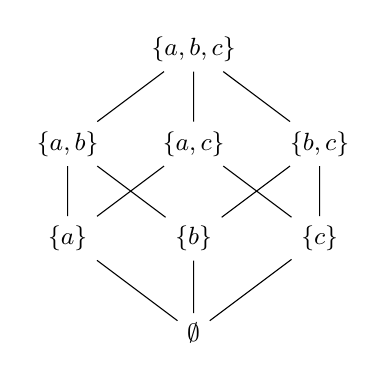
\begin{tikzpicture}[font=\small,node distance=1.1cm and 1.5cm]
  \node (e) at (0,0) {$\emptyset$};
  \node (a) at (-1.6,1.2) {$\{a\}$};
  \node (b) at (0,1.2) {$\{b\}$};
  \node (c) at (1.6,1.2) {$\{c\}$};
  \node (ab) at (-1.6,2.4) {$\{a,b\}$};
  \node (ac) at (0,2.4) {$\{a,c\}$};
  \node (bc) at (1.6,2.4) {$\{b,c\}$};
  \node (abc) at (0,3.6) {$\{a,b,c\}$};
  \draw (e)--(a) (e)--(b) (e)--(c) (a)--(ab) (a)--(ac) (b)--(ab) (b)--(bc) (c)--(ac) (c)--(bc) (ab)--(abc) (ac)--(abc) (bc)--(abc);
\end{tikzpicture}
\caption{Diagrama de Hasse de $(\Pa(\{a,b,c\}),\subseteq)$. El mínimo es $\emptyset$ y el máximo, $\{a,b,c\}$.}
\label{fig:t5-hasse}
\end{figure}

\begin{observacion}[Conexión con el curso]
Normalizar texto (pasar a minúsculas, aplicar una forma normal de Unicode) define el núcleo de una función y, por la \cref{prop:t5-nucleo}, una relación de equivalencia: dos cadenas son equivalentes si se normalizan igual (módulo~12, tema~1); la deduplicación de corpus agrupa documentos en clases de «casi duplicados» (módulo~16). Las relaciones de orden aparecen en el grafo computacional de una red, cuyo orden topológico es un orden total compatible con un orden parcial (módulo~10); en la atención causal, la posición $i$ solo atiende a las posiciones $j\le i$ (módulo~13); y BPE desempata entre pares igual de frecuentes con un orden total fijado (módulo~12, §2.3).
\end{observacion}

\begin{observacion}[Errores frecuentes]
(1) Creer que la simetría y la transitividad implican la reflexividad: el argumento «$a\sim b$ y $b\sim a$ dan $a\sim a$» exige que exista algún $b$ relacionado con $a$ (\cref{eje:5-error}). (2) Tratar simetría y antisimetría como contrarias. (3) Confundir elemento minimal con mínimo: en $\{2,3,4,6\}$ ordenado por divisibilidad, $2$ y $3$ son minimales y no hay mínimo. (4) Olvidar comprobar que una operación sobre clases no depende del representante elegido.
\end{observacion}

\begin{lecturas}
\item Hammack~\cite{hammack}, cap.~11 «Relations», §11.1–11.5.
\item Velleman~\cite{velleman}, §4.2 «Relations», §4.4 «Ordering Relations» y §4.5 «Equivalence Relations».
\item Lehman, Leighton y Meyer~\cite{mcs}, §4.4 «Binary Relations», §9.6 «Partial Orders», §9.8 «Linear Orders» y §9.10 «Equivalence Relations».
\end{lecturas}

\section*{Ejercicios del tema 5}
\addcontentsline{toc}{section}{Ejercicios del tema 5}

\begin{ejercicio}{1}{eje:5-propiedades}
En $A=\{1,2,3\}$ se consideran $R_1=\{(1,1),(2,2),(3,3),(1,2),(2,1)\}$, $R_2=\{(1,2),(2,3),(1,3)\}$, $R_3=\{(1,1),(2,2),(3,3)\}$ y $R_4=\{(1,2),(2,1)\}$. Decida para cada una si es reflexiva, simétrica, antisimétrica y transitiva.
\end{ejercicio}

\begin{ejercicio}{2}{eje:5-enteros}
Estudie las cuatro propiedades de la \cref{def:t5-prop} para las relaciones en $\Z$: (a) $a\,R\,b$ si $a+b$ es par; (b) $a\,R\,b$ si $ab\ge0$; (c) $a\,R\,b$ si $\abs{a-b}\le1$. ¿Cuál es de equivalencia? Describa sus clases.
\fuente{adaptado de Hammack~\cite{hammack}, §11.2 «Properties of Relations», ejercicios de la sección.}
\end{ejercicio}

\begin{ejercicio}{2}{eje:5-contar}
Sea $A$ un conjunto con $n=3$ elementos. ¿Cuántas relaciones hay en $A$? ¿Cuántas son reflexivas? ¿Cuántas simétricas? ¿Cuántas reflexivas y simétricas a la vez? Dé las fórmulas para $n$ general.
\end{ejercicio}

\begin{ejercicio}{2}{eje:5-clases}
Describa las clases de equivalencia y el conjunto cociente de: (a) la congruencia módulo~4 en $\Z$; (b) la relación en $\R^{2}$ «estar a la misma distancia del origen»; (c) la relación «tener la misma longitud» en $\{\cad{a},\cad{b}\}^{*}$, indicando cuántos elementos tiene cada clase.
\end{ejercicio}

\begin{ejercicio}{2}{eje:5-particion}
Sea $A=\{1,2,3,4,5,6\}$ y la partición $\{\{1,2\},\{3\},\{4,5,6\}\}$. Escriba los pares de la relación de equivalencia asociada y cuente cuántos son. Generalice: si los bloques tienen tamaños $k_1,\dots,k_r$, ¿cuántos pares tiene la relación?
\end{ejercicio}

\begin{ejercicio}{2}{eje:5-bell}
¿Cuántas relaciones de equivalencia hay en $\{1,2,3\}$? ¿Y en $\{1,2,3,4\}$? Clasifíquelas según los tamaños de los bloques de la partición correspondiente.
\end{ejercicio}

\begin{ejercicio}{3}{eje:5-modn}
Sea $n\ge1$. Demuestre que la congruencia módulo $n$ es una relación de equivalencia en $\Z$ y que tiene exactamente $n$ clases, $[0],[1],\dots,[n-1]$.
\fuente{adaptado de Hammack~\cite{hammack}, §11.3 «Equivalence Relations» y §11.5 «The Integers Modulo $n$».}
\end{ejercicio}

\begin{ejercicio}{3}{eje:5-nucleo}
Sea $f\colon A\to B$. Demuestre la \cref{prop:t5-nucleo}: la relación $a\sim_f a'$ si $f(a)=f(a')$ es de equivalencia y sus clases son las fibras no vacías de $f$. Deduzca que $f$ es inyectiva si y solo si todas sus clases tienen un solo elemento.
\fuente{adaptado de University of Washington, Math 300~\cite{uw300}, «Problems on functions», problema~3.}
\end{ejercicio}

\begin{ejercicio}{3}{eje:5-divide}
En $\N_{\ge1}=\{1,2,3,\dots\}$ se define $a\,R\,b$ si $a\mid b$ o $b\mid a$. ¿Es $R$ una relación de equivalencia? Demuestre las propiedades que se cumplan y refute las que no.
\fuente{adaptado de Cambridge, IA Numbers and Sets~\cite{camns}, Example Sheet~1, pregunta~10.}
\end{ejercicio}

\begin{ejercicio}{3}{eje:5-mas3}
Sea $R$ la relación en $\Z$ dada por $a\,R\,b$ si $b=a+3$. Se dice que una relación $S$ \emph{contiene} a $R$ si $a\,R\,b$ implica $a\,S\,b$. ¿Cuántas relaciones de equivalencia en $\Z$ contienen a $R$? Demuestre la respuesta.
\fuente{adaptado de Cambridge, IA Numbers and Sets~\cite{camns}, Example Sheet~1, pregunta~11.}
\end{ejercicio}

\begin{ejercicio}{3}{eje:5-fracciones}
En $X=\Z\times(\Z\setminus\{0\})$ se define $(a,b)\sim(c,d)$ si $ad=bc$. Demuestre que $\sim$ es una relación de equivalencia y describa la clase de $(1,2)$. Explique por qué $X/{\sim}$ puede identificarse con $\Q$.
\end{ejercicio}

\begin{ejercicio}{3}{eje:5-orden-partes}
(a) Demuestre que $\subseteq$ es un orden parcial en $\Pa(A)$, y que no es total si $\abs{A}\ge2$. (b) Demuestre que la divisibilidad es un orden parcial en $\N_{\ge1}$ y que no es antisimétrica en $\Z$.
\fuente{adaptado de Velleman~\cite{velleman}, §4.4 «Ordering Relations».}
\end{ejercicio}

\begin{ejercicio}{2}{eje:5-hasse}
(a) Dibuje el diagrama de Hasse de los divisores positivos de~12 ordenados por divisibilidad e indique minimales, maximales, mínimo y máximo. (b) Ordene lexicográficamente las cadenas $\cad{ab}$, $\cad{a}$, $\cad{b}$, $\cad{ba}$, $\cad{aab}$ y $\vacia$ (con $\cad{a}<\cad{b}$ y con la convención de que un prefijo propio precede a la cadena que lo contiene).
\end{ejercicio}

\begin{ejercicio}{3}{eje:5-lex}
Demuestre que el orden lexicográfico en $\N\times\N$ del \cref{ej:t5-ordenes} es un orden total. ¿Es un orden total el orden producto, $(a,b)\sqsubseteq(c,d)$ si $a\le c$ y $b\le d$?
\end{ejercicio}

\begin{ejercicio}{1}{eje:5-error}
Se afirma: «toda relación simétrica y transitiva es reflexiva, porque si $a\,R\,b$, la simetría da $b\,R\,a$ y la transitividad da $a\,R\,a$». Señale el error y dé un contraejemplo en $A=\{1,2\}$.
\end{ejercicio}

% =====================================================================
\chapter{Cardinalidad, palomar y diagonal de Cantor}
\label{tema:6}
% =====================================================================

Las funciones inyectivas, sobreyectivas y biyectivas permiten comparar el tamaño de dos conjuntos sin contar sus elementos. En conjuntos finitos esta comparación da el principio del palomar; en conjuntos infinitos conduce a la distinción entre conjuntos numerables y no numerables y al argumento diagonal de Cantor. El tema sigue la sección~12.3 y el capítulo~14 de Hammack~\cite{hammack}, el capítulo~8 de Velleman~\cite{velleman}, las secciones~4.5, 7.1 y~14.8 de~\cite{mcs} y las transparencias «Cardinality» de Stanford CS103~\cite{cs103card}.

\section{Comparar tamaños con funciones}

\begin{definicion}[Equipotencia]
Dos conjuntos $A$ y $B$ tienen el \emph{mismo cardinal}, y se escribe $\abs{A}=\abs{B}$, si existe una biyección $A\to B$. Se escribe $\abs{A}\le\abs{B}$ si existe una función inyectiva $A\to B$.
\end{definicion}

Para conjuntos finitos, estas definiciones coinciden con contar elementos (\cref{prop:t3-finitos}). La relación «tener el mismo cardinal» es reflexiva ($\id_A$ es biyectiva), simétrica (la inversa de una biyección es biyectiva, \cref{prop:t4-inv-comp}) y transitiva (la composición de biyecciones es biyectiva, \cref{teo:t4-comp}).

\begin{ejemplo}[Un conjunto infinito y una parte propia]\label{ej:t6-pares}
Sea $2\N=\{0,2,4,\dots\}$. La función $f\colon\N\to2\N$, $f(n)=2n$, es biyectiva: es inyectiva porque $2n=2m$ implica $n=m$, y sobreyectiva porque cada par $2k$ es $f(k)$. Por tanto $\abs{\N}=\abs{2\N}$ aunque $2\N\subsetneq\N$. Para conjuntos finitos esto es imposible: una parte propia tiene estrictamente menos elementos.
\end{ejemplo}

\section{El principio del palomar}

\begin{teorema}[Principio del palomar]\label{teo:t6-palomar}
Sean $A$ y $B$ finitos y $f\colon A\to B$.
\begin{enumerate}
  \item Si $\abs{A}>\abs{B}$, $f$ no es inyectiva: existen $a\neq a'$ con $f(a)=f(a')$.
  \item (Forma general.) Si $\abs{A}>k\abs{B}$ con $k\in\N$, alguna fibra tiene al menos $k+1$ elementos. En particular, alguna fibra tiene al menos $\lceil\abs{A}/\abs{B}\rceil$ elementos.
\end{enumerate}
\end{teorema}

\begin{proof}
(ii) Si todas las fibras tuvieran a lo sumo $k$ elementos, se tendría $\abs{A}=\sum_{b\in B}\abs{f^{-1}(\{b\})}\le k\abs{B}$, en contra de la hipótesis. El apartado~(i) es el caso $k=1$. Para la última afirmación, sea $m$ el tamaño de la mayor fibra; entonces $\abs{A}\le m\abs{B}$, luego $m\ge\abs{A}/\abs{B}$ y, por ser entero, $m\ge\lceil\abs{A}/\abs{B}\rceil$.
\end{proof}

El nombre procede de la imagen de $\abs{A}$ palomas que se refugian en $\abs{B}$ palomares: si hay más palomas que palomares, en algún palomar hay al menos dos. La dificultad en las aplicaciones está en elegir bien las «palomas» y los «palomares».

\begin{ejemplo}[Restos]\label{ej:t6-restos}
Entre cinco enteros cualesquiera hay dos cuya diferencia es múltiplo de~4. Palomas: los cinco enteros; palomares: los cuatro restos posibles al dividir entre~4. Dos enteros con el mismo resto tienen diferencia múltiplo de~4.
\end{ejemplo}

\begin{proposicion}[Límite de la compresión sin pérdida]\label{prop:t6-compresion}
Para $n\ge1$ no existe ninguna función inyectiva de $\{0,1\}^{n}$ en el conjunto $\{0,1\}^{<n}=\bigcup_{k=0}^{n-1}\{0,1\}^{k}$ de cadenas binarias de longitud menor que $n$.
\end{proposicion}

\begin{proof}
$\abs{\{0,1\}^{n}}=2^{n}$, mientras que $\abs{\{0,1\}^{<n}}=\sum_{k=0}^{n-1}2^{k}=2^{n}-1$. Por el \cref{teo:t6-palomar}(i), ninguna función entre ellos es inyectiva.
\end{proof}

Un compresor sin pérdida es una función inyectiva (debe poder descomprimirse). La \cref{prop:t6-compresion} dice que ningún compresor acorta \emph{todas} las cadenas de longitud $n$: si acorta algunas, alarga o deja igual otras. El módulo~6 cuantifica esta idea con la entropía.

\section{Conjuntos numerables}

\begin{definicion}[Numerable]
Un conjunto $A$ es \emph{infinito numerable} si $\abs{A}=\abs{\N}$, es decir, si sus elementos pueden listarse como $a_0,a_1,a_2,\dots$ sin repeticiones y sin omitir ninguno. Es \emph{numerable} si es finito o infinito numerable, y \emph{no numerable} en otro caso.
\end{definicion}

\begin{proposicion}\label{prop:t6-numerables}
Los conjuntos $\Z$, $\N\times\N$ y $\Sigma^{*}$ (con $\Sigma$ finito y no vacío) son infinitos numerables.
\end{proposicion}

\begin{proof}
\emph{El conjunto $\Z$.} La función del \cref{eje:3-NZ} es una biyección $\N\to\Z$, que da la lista $0$, $-1$, $1$, $-2$, $2$, \dots

\emph{El conjunto $\N\times\N$.} Se recorren los pares por diagonales $m+n=0,1,2,\dots$, y dentro de cada diagonal por orden creciente de $n$. La diagonal $m+n=d$ tiene $d+1$ pares, y las anteriores contienen $1+2+\dots+d=d(d+1)/2$; por tanto, el par $(m,n)$ ocupa la posición
\[
\pi(m,n)=\frac{(m+n)(m+n+1)}{2}+n.
\]
Cada natural $N$ se alcanza exactamente una vez: hay un único $d$ con $d(d+1)/2\le N<(d+1)(d+2)/2$, y entonces $n=N-d(d+1)/2\in\{0,\dots,d\}$ y $m=d-n$. Luego $\pi$ es una biyección (la \emph{función de emparejamiento de Cantor}).

\emph{El conjunto $\Sigma^{*}$.} Se listan las cadenas por longitud creciente y, dentro de cada longitud, en orden lexicográfico (\emph{orden de longitud y lexicográfico}). Cada longitud aporta un número finito $\abs{\Sigma}^{T}$ de cadenas, de modo que toda cadena aparece en una posición finita.
\end{proof}

\begin{figure}[h]
\centering
\begin{tikzpicture}[scale=0.8,font=\small,>={Stealth[length=1.6mm]}]
  \foreach \m in {0,...,3} \foreach \n in {0,...,3} {
    \pgfmathtruncatemacro{\d}{\m+\n}
    \pgfmathtruncatemacro{\p}{\d*(\d+1)/2+\n}
    \node[circle,draw,inner sep=1.5pt,minimum size=6mm] (p\m\n) at (\n*1.3,-\m*1.0) {\p};}
  \foreach \m in {0,...,3} \node[anchor=east] at (-0.55,-\m*1.0) {$m=\m$};
  \foreach \n in {0,...,3} \node at (\n*1.3,0.8) {$n=\n$};
  \draw[->,gray] (p10) -- (p01);
  \draw[->,gray] (p20) -- (p11); \draw[->,gray] (p11) -- (p02);
  \draw[->,gray] (p30) -- (p21); \draw[->,gray] (p21) -- (p12); \draw[->,gray] (p12) -- (p03);
\end{tikzpicture}
\caption{Recorrido de $\N\times\N$ por diagonales. Cada círculo muestra la posición $\pi(m,n)$ del par $(m,n)$.}
\label{fig:t6-cantor}
\end{figure}

\begin{proposicion}\label{prop:t6-criterios}
Sea $A$ un conjunto no vacío. Son equivalentes: (i) $A$ es numerable; (ii) existe una función inyectiva $A\to\N$; (iii) existe una función sobreyectiva $\N\to A$. Además, todo subconjunto de un conjunto numerable es numerable, y la unión de una familia numerable de conjuntos numerables es numerable.
\end{proposicion}

Se admite este resultado sin demostración completa (véase~\cite[§14.2]{hammack} y~\cite[§8.2]{velleman}); algunas de sus partes se piden en los \cref{eje:6-subconjN,eje:6-producto}. Como consecuencia, $\Q$ es numerable (\cref{eje:6-Q}).

\section{El argumento diagonal de Cantor}

\begin{teorema}[Cantor]\label{teo:t6-cantor}
Para todo conjunto $A$ no existe ninguna función sobreyectiva $A\to\Pa(A)$. En consecuencia, $\abs{A}\neq\abs{\Pa(A)}$.
\end{teorema}

\begin{proof}
Sea $f\colon A\to\Pa(A)$ una función cualquiera. Se considera el conjunto «diagonal»
\[
D=\{x\in A: x\notin f(x)\}\subseteq A.
\]
Supóngase que $D=f(y)$ para algún $y\in A$. Si $y\in D$, por la definición de $D$, $y\notin f(y)=D$; si $y\notin D$, entonces $y\notin f(y)$ y, por la definición de $D$, $y\in D$. Ambos casos son contradictorios, luego $D$ no es imagen de ningún elemento y $f$ no es sobreyectiva.
\end{proof}

\begin{corolario}\label{cor:t6-nonum}
$\Pa(\N)$ y el conjunto $\{0,1\}^{\N}$ de sucesiones infinitas de ceros y unos no son numerables.
\end{corolario}

\begin{proof}
Por el \cref{teo:t6-cantor}, no hay biyección $\N\to\Pa(\N)$, y $\Pa(\N)$ es infinito; luego no es numerable. La función $X\mapsto\chi_X$ es una biyección $\Pa(\N)\to\{0,1\}^{\N}$ (\cref{tema:2}), así que $\{0,1\}^{\N}$ tampoco es numerable.
\end{proof}

El nombre «diagonal» se entiende con sucesiones: dada una lista $s_0,s_1,s_2,\dots$ de sucesiones binarias, la sucesión $d$ con $d_k=1-s_k(k)$ difiere de $s_k$ en la posición $k$, luego no está en la lista. El mismo argumento, con desarrollos decimales y evitando las colas de nueves, prueba que $\R$ no es numerable~\cite[§14.2]{hammack}.

\begin{observacion}[Conexión con el curso]
El conjunto $\V^{*}$ de todos los textos tokenizados es infinito numerable (\cref{prop:t6-numerables}); por eso un modelo de lenguaje es una distribución \emph{discreta} y la condición de normalización es una serie (módulo~1, §1.3; módulo~5). El principio del palomar explica por qué un identificador de token de 15~bits no basta para un vocabulario de $5\cdot10^{4}$ tokens (módulo~12) y por qué toda función \emph{hash} sobre un conjunto mayor que su rango produce colisiones (módulo~16). Por último, los números en coma flotante forman un conjunto \emph{finito} (módulo~11): una red implementada en un ordenador es una función entre conjuntos finitos, aunque se modele con funciones reales.
\end{observacion}

\begin{observacion}[Errores frecuentes]
(1) Pensar que una parte propia de un conjunto infinito es siempre «más pequeña» (\cref{ej:t6-pares}). (2) Creer que todos los conjuntos infinitos tienen el mismo cardinal: $\abs{\N}<\abs{\Pa(\N)}$. (3) Aplicar el palomar sin identificar con precisión la función de las palomas a los palomares. (4) En el argumento diagonal con decimales, olvidar que $0{,}0999\ldots=0{,}1$: hay que elegir dígitos que eviten esa ambigüedad.
\end{observacion}

\begin{lecturas}
\item Hammack~\cite{hammack}, §3.9 «The Division and Pigeonhole Principles», §12.3 «The Pigeonhole Principle Revisited» y cap.~14 «Cardinality of Sets», §14.1–14.3.
\item Velleman~\cite{velleman}, §8.1 «Equinumerous Sets» y §8.2 «Countable and Uncountable Sets».
\item Lehman, Leighton y Meyer~\cite{mcs}, §4.5 «Finite Cardinality», §7.1 «Infinite Cardinality» y §14.8 «The Pigeonhole Principle».
\item Stanford CS103~\cite{cs103card}, transparencias «Cardinality».
\end{lecturas}

\section*{Ejercicios del tema 6}
\addcontentsline{toc}{section}{Ejercicios del tema 6}

\begin{ejercicio}{1}{eje:6-vf}
Decida si son verdaderas o falsas, justificando con un resultado del tema: (a) si $A\subsetneq B$, entonces $\abs{A}<\abs{B}$; (b) $\abs{\N}=\abs{2\N}$; (c) $\Q$ es numerable; (d) $\Pa(\N)$ es numerable; (e) existe una biyección entre $\Z$ y $\N\times\N$.
\end{ejercicio}

\begin{ejercicio}{1}{eje:6-textos}
¿Hay más textos posibles (elementos de $\V^{*}$, con $\V$ finito) que números naturales? ¿Más que números reales? ¿Y más que números en coma flotante de 32~bits? Justifique cada respuesta.
\end{ejercicio}

\begin{ejercicio}{2}{eje:6-meses}
(a) En un grupo de 13 personas, ¿hay necesariamente dos nacidas el mismo mes? (b) ¿Cuántas personas hacen falta para garantizar que tres hayan nacido el mismo mes? (c) Se extraen calcetines de un cajón con calcetines de 4 colores; ¿cuántos hay que extraer para garantizar un par del mismo color?
\end{ejercicio}

\begin{ejercicio}{2}{eje:6-bits}
(a) Un vocabulario tiene $K=5\cdot10^{4}$ tokens. Demuestre que los identificadores no caben en 15~bits y calcule el número mínimo de bits necesario. (b) Se asignan $10^{6}$ palabras a $2^{16}$ cubetas de una tabla \emph{hash}. Demuestre que alguna cubeta recibe al menos 16 palabras.
\end{ejercicio}

\begin{ejercicio}{3}{eje:6-restos}
(a) Demuestre que entre $n+1$ enteros cualesquiera hay dos cuya diferencia es múltiplo de $n$. (b) Demuestre que si se eligen $n+1$ números del conjunto $\{1,2,\dots,2n\}$, dos de ellos son consecutivos.
\end{ejercicio}

\begin{ejercicio}{3}{eje:6-puntos}
Demuestre que entre cinco puntos cualesquiera del plano con coordenadas enteras hay dos cuyo punto medio tiene también coordenadas enteras. ¿Es cierto con cuatro puntos?
\end{ejercicio}

\begin{ejercicio}{3}{eje:6-compresion}
(a) Demuestre la \cref{prop:t6-compresion}. (b) Sea $C\colon\{0,1\}^{*}\to\{0,1\}^{*}$ una función inyectiva. Demuestre que para cada $n\ge1$ existe una cadena $w$ de longitud $n$ con $\abs{C(w)}\ge n$.
\end{ejercicio}

\begin{ejercicio}{2}{eje:6-pi}
Con la función de emparejamiento $\pi(m,n)=\tfrac{(m+n)(m+n+1)}{2}+n$: (a) calcule $\pi(2,3)$ y $\pi(0,4)$; (b) halle el par $(m,n)$ con $\pi(m,n)=17$; (c) compruebe en la \cref{fig:t6-cantor} los valores de la diagonal $m+n=3$.
\end{ejercicio}

\begin{ejercicio}{2}{eje:6-shortlex}
Sea $\Sigma=\{\cad{a},\cad{b}\}$ con $\cad{a}<\cad{b}$. (a) Escriba las 14 primeras cadenas de $\Sigma^{*}$ en el orden de longitud y lexicográfico, numeradas desde~0. (b) ¿En qué posición aparece $\cad{bab}$? (c) Demuestre que, si se lee $\cad{a}$ como 0 y $\cad{b}$ como 1, la cadena de longitud $L$ cuyo valor binario es $v$ ocupa la posición $2^{L}-1+v$.
\end{ejercicio}

\begin{ejercicio}{2}{eje:6-diagonal}
Las cinco primeras sucesiones binarias de una supuesta lista de $\{0,1\}^{\N}$ empiezan así: $s_0=10110\ldots$, $s_1=00101\ldots$, $s_2=11100\ldots$, $s_3=01011\ldots$, $s_4=11111\ldots$. Escriba los cinco primeros términos de la sucesión diagonal $d$, con $d_k=1-s_k(k)$, y compruebe que $d$ difiere de cada $s_k$, $k\le4$.
\end{ejercicio}

\begin{ejercicio}{3}{eje:6-subconjN}
Demuestre que todo subconjunto infinito $S\subseteq\N$ es infinito numerable: construya una biyección $\N\to S$ que liste los elementos de $S$ en orden creciente.
\fuente{adaptado de Cambridge, Discrete Mathematics~\cite{camdm}, hoja~8, ejercicio~13.2.1.}
\end{ejercicio}

\begin{ejercicio}{3}{eje:6-producto}
(a) Demuestre que $g\colon\N\times\N\to\N$, $g(m,n)=2^{m}(2n+1)-1$, es biyectiva. (b) Deduzca que si $A$ y $B$ son infinitos numerables, $A\times B$ también lo es.
\fuente{adaptado de Cambridge, Discrete Mathematics~\cite{camdm}, hoja~8, ejercicio~13.2.3.}
\end{ejercicio}

\begin{ejercicio}{3}{eje:6-Q}
Demuestre que $\Q$ es numerable. Puede usar que todo racional se escribe de forma única como $p/q$ con $p\in\Z$, $q\in\N$, $q\ge1$ y $\operatorname{mcd}(\abs{p},q)=1$, y la \cref{prop:t6-criterios}.
\fuente{adaptado de Cambridge, Discrete Mathematics~\cite{camdm}, hoja~8, ejercicio~13.1.2.}
\end{ejercicio}

\begin{ejercicio}{3}{eje:6-PA}
Sea $A$ un conjunto cualquiera. Demuestre que no existe ninguna función inyectiva $\Pa(A)\to A$.
\fuente{adaptado de Cambridge, Discrete Mathematics~\cite{camdm}, hoja~8, ejercicio~13.2.4.}
\end{ejercicio}

\begin{ejercicio}{3}{eje:6-intervalos}
(a) Demuestre que $f\colon[0,1]\to[0,2]$, $f(x)=2x$, es biyectiva. (b) Construya una biyección $[0,1]\to(0,1)$ y demuestre que lo es. (Indicación: envíe $0\mapsto\tfrac12$ y $\tfrac1n\mapsto\tfrac1{n+2}$ para $n\ge1$, y deje fijos los demás puntos.)
\fuente{adaptado de Stanford CS103~\cite{cs103ps3}, Problem Set~3, problema~7 «Infinity Minus Two».}
\end{ejercicio}


\appendix
% =====================================================================
\chapter{Soluciones de los ejercicios}
\label{ap:soluciones}
% =====================================================================

Cada solución se presenta en cinco partes: datos, planteamiento, desarrollo, resultado y comprobación. En los ejercicios de demostración, los datos son las hipótesis y el resultado es el enunciado demostrado; la comprobación consiste en un caso particular o en una verificación independiente. Los recuentos se han comprobado por enumeración exhaustiva con un programa.

% ---------------------------------------------------------------------
\section{Tema 1}

\begin{solucion}{eje:1-pert}
\datos $A=\{1,\{1\},\{1,2\}\}$, cuyos tres elementos son $1$, $\{1\}$ y $\{1,2\}$.
\planteamiento $x\in A$ exige que $x$ sea uno de los tres elementos; $X\subseteq A$ exige que \emph{cada} elemento de $X$ sea uno de ellos.
\pasos
\begin{enumerate}[label=(\alph*)]
  \item $1$ es elemento de $A$: \textbf{verdadera}.
  \item $\{1\}$ es elemento de $A$: \textbf{verdadera}.
  \item El único elemento de $\{1\}$ es $1\in A$: \textbf{verdadera}.
  \item El elemento $2$ de $\{2\}$ no está en $A$: \textbf{falsa}.
  \item $\{1,2\}$ es elemento de $A$: \textbf{verdadera}.
  \item El único elemento de $\{\{1,2\}\}$ es $\{1,2\}\in A$: \textbf{verdadera}.
  \item $\emptyset$ es subconjunto de todo conjunto (\cref{prop:t1-subconj}): \textbf{verdadera}.
  \item $\emptyset$ no es ninguno de los tres elementos: \textbf{falsa}.
\end{enumerate}
\resultado verdaderas (a), (b), (c), (e), (f), (g); falsas (d), (h).
\comprobacion los apartados (b) y (c) muestran que un mismo objeto, $\{1\}$, puede ser a la vez elemento y subconjunto de $A$.
\end{solucion}

\begin{solucion}{eje:1-card}
\planteamiento contar los elementos distintos, sin mirar dentro de los elementos que son conjuntos.
\pasos
\begin{enumerate}[label=(\alph*)]
  \item $\{\emptyset\}$ tiene un elemento: $1$.
  \item $\emptyset$ y $\{\emptyset\}$ son distintos (uno vacío, otro no): $2$.
  \item $\Pa(\emptyset)=\{\emptyset\}$: $1=2^{0}$.
  \item $\Pa(\Pa(\emptyset))=\Pa(\{\emptyset\})=\{\emptyset,\{\emptyset\}\}$: $2=2^{1}$.
  \item $\{1,2\}=\{2,1\}$, luego el conjunto es $\{\{1,2\}\}$: $1$.
  \item $1$, $\{1\}$ y $\{\{1\}\}$ son distintos: $3$.
\end{enumerate}
\resultado $1,\ 2,\ 1,\ 2,\ 1,\ 3$.
\comprobacion (c) y (d) concuerdan con el \cref{teo:t1-partes}: $\abs{\Pa(A)}=2^{\abs{A}}$ con $\abs{A}=0$ y $\abs{A}=1$.
\end{solucion}

\begin{solucion}{eje:1-extension}
\datos $A=\{x\in\Z: x^{2}<10\}$, $B$ = divisores positivos de 12, $C$ = raíces de $x^{2}-3x+2$.
\planteamiento escribir cada conjunto por extensión y aplicar las definiciones.
\pasos
\begin{enumerate}[label=\arabic*.]
  \item $x^{2}<10$ con $x$ entero: $\abs{x}\le3$ porque $3^{2}=9<10\le16=4^{2}$. $A=\{-3,-2,-1,0,1,2,3\}$.
  \item $B=\{1,2,3,4,6,12\}$.
  \item $x^{2}-3x+2=(x-1)(x-2)$: $C=\{1,2\}$.
  \item $A\cap B=\{1,2,3\}$; $A\setminus B=\{-3,-2,-1,0\}$; $B\setminus A=\{4,6,12\}$.
  \item $A\dsim B=(A\setminus B)\cup(B\setminus A)=\{-3,-2,-1,0,4,6,12\}$.
  \item $(A\cap B)\setminus C=\{1,2,3\}\setminus\{1,2\}=\{3\}$.
\end{enumerate}
\resultado $A\cap B=\{1,2,3\}$, $A\setminus B=\{-3,-2,-1,0\}$, $B\setminus A=\{4,6,12\}$, $A\dsim B=\{-3,-2,-1,0,4,6,12\}$, $(A\cap B)\setminus C=\{3\}$.
\comprobacion $\abs{A\dsim B}=\abs{A}+\abs{B}-2\abs{A\cap B}=7+6-6=7$.
\end{solucion}

\begin{solucion}{eje:1-partes}
\datos $A=\{a,b,c\}$, $\abs{A}=3$.
\planteamiento listar por tamaños y contar.
\pasos
\begin{enumerate}[label=\arabic*.]
  \item $\Pa(A)=\{\emptyset,\{a\},\{b\},\{c\},\{a,b\},\{a,c\},\{b,c\},\{a,b,c\}\}$: 8 elementos.
  \item Contienen a $a$: $\{a\},\{a,b\},\{a,c\},\{a,b,c\}$, es decir, 4.
  \item Con dos elementos: $\{a,b\},\{a,c\},\{b,c\}$, es decir, 3.
  \item En general, $X\mapsto X\setminus\{a\}$ hace corresponder los subconjuntos que contienen a $a$ con los subconjuntos de $A\setminus\{a\}$, uno a uno (la operación inversa es añadir $a$). Hay $2^{n-1}$.
\end{enumerate}
\resultado 8 subconjuntos; 4 contienen a $a$; 3 tienen dos elementos; en general, $2^{n-1}$ contienen a $a$.
\comprobacion $2^{3-1}=4$; además los que no contienen a $a$ son otros $4$ y $4+4=8$.
\end{solucion}

\begin{solucion}{eje:1-cartesiano}
\datos $A=\{0,1\}$, $B=\{\cad{a},\cad{b},\cad{c}\}$.
\planteamiento \cref{prop:t1-producto}.
\pasos
\begin{enumerate}[label=(\alph*)]
  \item $A\times B=\{(0,\cad{a}),(0,\cad{b}),(0,\cad{c}),(1,\cad{a}),(1,\cad{b}),(1,\cad{c})\}$.
  \item $\abs{A^{3}}=2^{3}=8$; $\abs{B\times A\times A}=3\cdot2\cdot2=12$.
  \item No: $(0,\cad{a})\in A\times B$, pero $(0,\cad{a})\notin B\times A$, cuyos pares tienen primera componente en $B$.
  \item $A^{8}$ es el conjunto de las cadenas de 8 bits, es decir, de los bytes: $\abs{A^{8}}=2^{8}=256$.
\end{enumerate}
\resultado 6 pares; $8$ y $12$; $A\times B\neq B\times A$; hay $256$ bytes distintos.
\comprobacion $\abs{A\times B}=2\cdot3=6$ coincide con la lista de~(a).
\end{solucion}

\begin{solucion}{eje:1-demorgan-num}
\datos $U=\{1,\dots,10\}$, $A=\{1,2,3,4,5\}$, $B=\{2,4,6,8,10\}$, $C=\{3,4,5,6\}$.
\planteamiento calcular cada miembro por separado.
\pasos
\begin{enumerate}[label=\arabic*.]
  \item $A\cup B=\{1,2,3,4,5,6,8,10\}$, luego $\overline{A\cup B}=\{7,9\}$.
  \item $\overline{A}=\{6,7,8,9,10\}$, $\overline{B}=\{1,3,5,7,9\}$, luego $\overline{A}\cap\overline{B}=\{7,9\}$.
  \item $B\cap C=\{4,6\}$, luego $A\setminus(B\cap C)=\{1,2,3,5\}$.
  \item $A\setminus B=\{1,3,5\}$ y $A\setminus C=\{1,2\}$, luego $(A\setminus B)\cup(A\setminus C)=\{1,2,3,5\}$.
  \item Coinciden porque, por el \cref{teo:t1-leyes}, $A\setminus(B\cap C)=A\cap\overline{B\cap C}=A\cap(\overline{B}\cup\overline{C})=(A\cap\overline{B})\cup(A\cap\overline{C})$, que es $(A\setminus B)\cup(A\setminus C)$.
\end{enumerate}
\resultado $\overline{A\cup B}=\overline{A}\cap\overline{B}=\{7,9\}$; $A\setminus(B\cap C)=(A\setminus B)\cup(A\setminus C)=\{1,2,3,5\}$.
\comprobacion $7$ y $9$ son los únicos números de $U$ que no son pares ni están entre 1 y~5.
\end{solucion}

\begin{solucion}{eje:1-vf}
\planteamiento buscar contraejemplos pequeños; si no aparecen, intentar una demostración.
\pasos
\begin{enumerate}[label=(\alph*)]
  \item \textbf{Falsa.} Con $A=\{1,2\}$, $B=\{2\}$: $(A\cup B)\setminus B=\{1\}\neq A$.
  \item \textbf{Verdadera.} Es el \cref{ej:t1-doble}.
  \item \textbf{Falsa.} Con $A=B=\{1\}$ y $C=D=\{2\}$: el miembro izquierdo es $\{(1,1),(2,2)\}$; el derecho, $\{1,2\}\times\{1,2\}$, contiene además $(1,2)$ y $(2,1)$. Solo se cumple la inclusión $\subseteq$.
\end{enumerate}
\resultado (a) falsa; (b) verdadera; (c) falsa.
\comprobacion en (c), los cardinales $2$ y $4$ ya muestran que los conjuntos son distintos.
\end{solucion}

\begin{solucion}{eje:1-dif-union}
\datos $A,B,C$ conjuntos arbitrarios.
\planteamiento doble inclusión (\cref{prop:t1-subconj}(iii)).
\pasos
\begin{enumerate}[label=\arabic*.]
  \item ($\subseteq$) Sea $x\in A\setminus(B\cup C)$. Entonces $x\in A$ y $x\notin B\cup C$, es decir, $x\notin B$ y $x\notin C$. Por tanto $x\in A\setminus B$ y $x\in A\setminus C$, y $x$ está en la intersección.
  \item ($\supseteq$) Sea $x\in(A\setminus B)\cap(A\setminus C)$. Entonces $x\in A$, $x\notin B$ y $x\notin C$; luego $x\notin B\cup C$ y $x\in A\setminus(B\cup C)$.
\end{enumerate}
\resultado $A\setminus(B\cup C)=(A\setminus B)\cap(A\setminus C)$. \hfill$\blacksquare$
\comprobacion con los datos del \cref{eje:1-demorgan-num}: $A\setminus(B\cup C)=\{1\}$ y $(A\setminus B)\cap(A\setminus C)=\{1,3,5\}\cap\{1,2\}=\{1\}$.
\end{solucion}

\begin{solucion}{eje:1-union-inclusion}
\datos $A,B$ conjuntos arbitrarios.
\planteamiento probar las dos implicaciones; la igualdad $A\cup B=B$ se prueba por doble inclusión.
\pasos
\begin{enumerate}[label=\arabic*.]
  \item ($\Rightarrow$) Supóngase $A\subseteq B$. Siempre $B\subseteq A\cup B$. Recíprocamente, si $x\in A\cup B$, entonces $x\in A$ o $x\in B$; en el primer caso $x\in B$ por la hipótesis. Luego $A\cup B\subseteq B$ y hay igualdad.
  \item ($\Leftarrow$) Supóngase $A\cup B=B$. Si $x\in A$, entonces $x\in A\cup B=B$. Luego $A\subseteq B$.
  \item Análogo para la intersección: $A\subseteq B\iff A\cap B=A$. ($\Rightarrow$) $A\cap B\subseteq A$ siempre; si $x\in A$, entonces $x\in B$ por hipótesis y $x\in A\cap B$. ($\Leftarrow$) Si $x\in A=A\cap B$, entonces $x\in B$.
\end{enumerate}
\resultado $A\subseteq B\iff A\cup B=B\iff A\cap B=A$. \hfill$\blacksquare$
\comprobacion con $A=\{1\}$, $B=\{1,2\}$: $A\cup B=\{1,2\}=B$ y $A\cap B=\{1\}=A$.
\end{solucion}

\begin{solucion}{eje:1-producto-inter}
\datos $A,B,C$ conjuntos arbitrarios.
\planteamiento los elementos de un producto son pares; se trabaja con un par arbitrario $(x,y)$.
\pasos
\begin{enumerate}[label=\arabic*.]
  \item $(x,y)\in A\times(B\cap C)\iff x\in A$ y $y\in B$ y $y\in C\iff(x\in A$ y $y\in B)$ y $(x\in A$ y $y\in C)\iff(x,y)\in(A\times B)\cap(A\times C)$. Cada paso es una equivalencia, luego se tienen las dos inclusiones a la vez.
  \item ($\subseteq$) Sea $(x,y)\in(A\setminus B)\times C$: $x\in A$, $x\notin B$, $y\in C$. Entonces $(x,y)\in A\times C$, y $(x,y)\notin B\times C$ porque $x\notin B$.
  \item ($\supseteq$) Sea $(x,y)\in(A\times C)\setminus(B\times C)$: $x\in A$, $y\in C$ y no es cierto que ($x\in B$ y $y\in C$). Como $y\in C$, debe ser $x\notin B$. Luego $(x,y)\in(A\setminus B)\times C$.
\end{enumerate}
\resultado $A\times(B\cap C)=(A\times B)\cap(A\times C)$ y $(A\setminus B)\times C=(A\times C)\setminus(B\times C)$. \hfill$\blacksquare$
\comprobacion con $A=\{1,2\}$, $B=\{2\}$, $C=\{0\}$: $(A\setminus B)\times C=\{(1,0)\}$ y $(A\times C)\setminus(B\times C)=\{(1,0),(2,0)\}\setminus\{(2,0)\}=\{(1,0)\}$.
\end{solucion}

\begin{solucion}{eje:1-simetrica}
\datos $A,B,C$ conjuntos; $A\dsim B=(A\setminus B)\cup(B\setminus A)$.
\planteamiento (a) doble inclusión; (b) lectura de la definición; (c) traducir la pertenencia a paridades con funciones características (\cref{tema:2}).
\pasos
\begin{enumerate}[label=\arabic*.]
  \item (a, $\subseteq$) Si $x\in A\setminus B$, entonces $x\in A\cup B$ y $x\notin A\cap B$ (no está en $B$); igual si $x\in B\setminus A$.
  \item (a, $\supseteq$) Si $x\in A\cup B$ y $x\notin A\cap B$: si $x\in A$, entonces $x\notin B$ y $x\in A\setminus B$; si $x\in B$, entonces $x\notin A$ y $x\in B\setminus A$.
  \item (b) $x\in A\setminus B$ significa «en $A$ y no en $B$», y $x\in B\setminus A$, «en $B$ y no en $A$»: $x\in A\dsim B$ exactamente cuando está en uno y solo uno.
  \item (c) Por (b), $\chi_{A\dsim B}(x)=1$ si y solo si $\chi_A(x)+\chi_B(x)=1$, es decir, $\chi_{A\dsim B}=(\chi_A+\chi_B)\bmod 2$.
  \item Aplicándolo dos veces: $\chi_{(A\dsim B)\dsim C}=\bigl((\chi_A+\chi_B)\bmod2+\chi_C\bigr)\bmod2=(\chi_A+\chi_B+\chi_C)\bmod 2$. Del mismo modo, $\chi_{A\dsim(B\dsim C)}=(\chi_A+\chi_B+\chi_C)\bmod2$.
  \item Los dos conjuntos tienen la misma función característica, luego son iguales: ambos son los $x$ que pertenecen a un número \emph{impar} de los tres conjuntos.
\end{enumerate}
\resultado $A\dsim B=(A\cup B)\setminus(A\cap B)$ y $(A\dsim B)\dsim C=A\dsim(B\dsim C)$. \hfill$\blacksquare$
\comprobacion con $A=\{1,2\}$, $B=\{2,3\}$, $C=\{3,4\}$: $(A\dsim B)\dsim C=\{1,3\}\dsim\{3,4\}=\{1,4\}$ y $A\dsim(B\dsim C)=\{1,2\}\dsim\{2,4\}=\{1,4\}$.
\end{solucion}

\begin{solucion}{eje:1-partes-inter}
\datos $A,B$ conjuntos arbitrarios.
\planteamiento los elementos de $\Pa(\cdot)$ son conjuntos: se toma un conjunto arbitrario $X$.
\pasos
\begin{enumerate}[label=\arabic*.]
  \item $X\in\Pa(A)\cap\Pa(B)\iff X\subseteq A$ y $X\subseteq B$.
  \item Si $X\subseteq A$ y $X\subseteq B$, todo $x\in X$ está en $A$ y en $B$, luego $X\subseteq A\cap B$. Recíprocamente, si $X\subseteq A\cap B$, como $A\cap B\subseteq A$ y $A\cap B\subseteq B$, la transitividad da $X\subseteq A$ y $X\subseteq B$. Así $X\in\Pa(A)\cap\Pa(B)\iff X\in\Pa(A\cap B)$.
  \item Si $X\in\Pa(A)\cup\Pa(B)$, entonces $X\subseteq A$ o $X\subseteq B$; en ambos casos $X\subseteq A\cup B$, luego $X\in\Pa(A\cup B)$.
  \item Contraejemplo de la igualdad: $A=\{1\}$, $B=\{2\}$. Entonces $\{1,2\}\in\Pa(A\cup B)$, pero $\{1,2\}\not\subseteq A$ y $\{1,2\}\not\subseteq B$.
\end{enumerate}
\resultado $\Pa(A)\cap\Pa(B)=\Pa(A\cap B)$ y $\Pa(A)\cup\Pa(B)\subseteq\Pa(A\cup B)$, con inclusión estricta en general. \hfill$\blacksquare$
\comprobacion en el contraejemplo, $\abs{\Pa(A)\cup\Pa(B)}=\abs{\{\emptyset,\{1\},\{2\}\}}=3<4=\abs{\Pa(A\cup B)}$.
\end{solucion}

\begin{solucion}{eje:1-familias}
\datos $B_n=\{k\in\N: k\ge n\}$; intervalos $(\tfrac1n,2)$ y $(-\tfrac1n,\tfrac1n)$.
\planteamiento para la intersección infinita, suponer que un elemento está en todos los conjuntos y llegar a contradicción.
\pasos
\begin{enumerate}[label=\arabic*.]
  \item Los $B_n$ son decrecientes ($B_{n+1}\subseteq B_n$), luego $B_1\cap\dots\cap B_n=B_n$, que contiene a $n$: no es vacío.
  \item Si $k\in\bigcap_{n\ge1}B_n$, en particular $k\in B_{k+1}$, es decir, $k\ge k+1$: absurdo. Luego $\bigcap_{n\ge1}B_n=\emptyset$.
  \item Cada $(\tfrac1n,2)\subseteq(0,2)$. Si $x\in(0,2)$, se elige $n>1/x$; entonces $\tfrac1n<x$ y $x\in(\tfrac1n,2)$. Luego $\bigcup_{n\ge1}(\tfrac1n,2)=(0,2)$.
  \item $0$ está en todos los $(-\tfrac1n,\tfrac1n)$. Si $x\neq0$, se elige $n>1/\abs{x}$; entonces $\abs{x}>\tfrac1n$ y $x$ no está en el $n$-ésimo intervalo. Luego la intersección es $\{0\}$.
\end{enumerate}
\resultado $\bigcap B_n=\emptyset$ aunque toda intersección finita es no vacía; $\bigcup(\tfrac1n,2)=(0,2)$; $\bigcap(-\tfrac1n,\tfrac1n)=\{0\}$. \hfill$\blacksquare$
\comprobacion $0\notin\bigcup(\tfrac1n,2)$ porque $0<\tfrac1n$ para todo $n$, de acuerdo con el extremo abierto de $(0,2)$.
\end{solucion}

\begin{solucion}{eje:1-cadenas}
\datos $\Sigma=\{\cad{a},\cad{b}\}$; $L_1$: longitud $\le2$; $L_2$: empiezan por \cad{a}.
\planteamiento listar por longitudes.
\pasos
\begin{enumerate}[label=(\alph*)]
  \item $L_1=\{\vacia,\cad{a},\cad{b},\cad{aa},\cad{ab},\cad{ba},\cad{bb}\}$; $\abs{L_1}=1+2+4=7$.
  \item $L_1\cap L_2=\{\cad{a},\cad{aa},\cad{ab}\}$; $L_1\setminus L_2=\{\vacia,\cad{b},\cad{ba},\cad{bb}\}$ (la cadena vacía no empieza por \cad{a}).
  \item $L_2$ es infinito: contiene $\cad{a},\cad{aa},\cad{aaa},\dots$, todas distintas.
\end{enumerate}
\resultado $\abs{L_1}=7$; $L_1\cap L_2$ tiene 3 cadenas y $L_1\setminus L_2$ tiene~4; $L_2$ es infinito.
\comprobacion $3+4=7=\abs{L_1}$, como debe ser al partir $L_1$ en dos.
\end{solucion}

% ---------------------------------------------------------------------
\section{Tema 2}

\begin{solucion}{eje:2-esfuncion}
\planteamiento comprobar existencia y unicidad de la imagen (\cref{def:t2-funcion}) y, en (e), que la regla no dependa del representante.
\pasos
\begin{enumerate}[label=(\alph*)]
  \item Cada uno de $1,2,3$ aparece exactamente una vez: \textbf{es función}.
  \item El~3 no tiene imagen: \textbf{no es función} (falla la existencia).
  \item El~1 tiene dos imágenes: \textbf{no es función} (falla la unicidad).
  \item $0$ no tiene imagen en $\R$: \textbf{no es función} de $\R$ en $\R$ (sí lo es de $\R\setminus\{0\}$ en $\R$).
  \item $\tfrac12=\tfrac24$, pero $\tfrac{1+1}{2+1}=\tfrac23$ y $\tfrac{2+1}{4+1}=\tfrac35$: \textbf{no está bien definida}.
\end{enumerate}
\resultado solo (a) es función.
\comprobacion en (e), $\tfrac23\neq\tfrac35$ porque $2\cdot5=10\neq9=3\cdot3$.
\end{solucion}

\begin{solucion}{eje:2-tabla}
\datos $f(0)=2$, $f(1)=4$, $f(2)=2$, $f(3)=1$, $f(4)=2$; $B=\{1,2,3,4,5\}$.
\planteamiento \cref{def:t2-imagen}.
\pasos
\begin{enumerate}[label=\arabic*.]
  \item Cada elemento de $A$ aparece en un único par y las segundas componentes están en $B$: es función. Dominio $A$, codominio $B$, recorrido $f(A)=\{1,2,4\}$.
  \item $f(\{0,1,2\})=\{f(0),f(1),f(2)\}=\{2,4\}$.
  \item $f^{-1}(\{2\})=\{0,2,4\}$; $f^{-1}(\{3,5\})=\emptyset$; $f^{-1}(\{1,4\})=\{1,3\}$.
\end{enumerate}
\resultado recorrido $\{1,2,4\}$; $f(\{0,1,2\})=\{2,4\}$; preimágenes $\{0,2,4\}$, $\emptyset$, $\{1,3\}$.
\comprobacion las fibras $f^{-1}(\{1\})=\{3\}$, $f^{-1}(\{2\})=\{0,2,4\}$, $f^{-1}(\{4\})=\{1\}$ tienen $1+3+1=5=\abs{A}$ elementos.
\end{solucion}

\begin{solucion}{eje:2-contar}
\planteamiento \cref{prop:t2-contar}: $\abs{B^{A}}=\abs{B}^{\abs{A}}$.
\pasos
\begin{enumerate}[label=\arabic*.]
  \item De 3 en 4: $4^{3}=64$. De 4 en 3: $3^{4}=81$.
  \item $\abs{\{0,1\}^{2}}=4$, luego hay $2^{4}=16$ funciones booleanas de dos variables.
  \item $\abs{\{0,1\}^{n}}=2^{n}$, luego hay $2^{2^{n}}$; para $n=3$, $2^{8}=256$.
\end{enumerate}
\resultado $64$, $81$, $16$ y $2^{2^{n}}$ ($256$ para $n=3$).
\comprobacion entre las 16 funciones booleanas están las conocidas \textsc{and}, \textsc{or} y \textsc{xor}, y las dos constantes.
\end{solucion}

\begin{solucion}{eje:2-cuadrado}
\datos $f(x)=x^{2}-2x=(x-1)^{2}-1$.
\planteamiento completar el cuadrado: $f$ decrece en $(-\infty,1]$, crece en $[1,\infty)$ y tiene mínimo $-1$ en $x=1$.
\pasos
\begin{enumerate}[label=\arabic*.]
  \item En $[0,3]$: mínimo $f(1)=-1$; $f(0)=0$ y $f(3)=3$. Por continuidad, $f([0,3])=[-1,3]$.
  \item $f(x)=3\iff x^{2}-2x-3=0\iff(x-3)(x+1)=0$: $f^{-1}(\{3\})=\{-1,3\}$.
  \item $-1\le(x-1)^{2}-1\le0\iff0\le(x-1)^{2}\le1\iff\abs{x-1}\le1$: $f^{-1}([-1,0])=[0,2]$.
  \item $f(x)\ge-1>-2$ para todo $x$: $f^{-1}((-\infty,-2))=\emptyset$.
  \item $f(\{3\})=\{3\}$, luego $f^{-1}(f(\{3\}))=\{-1,3\}\supsetneq\{3\}$.
\end{enumerate}
\resultado $[-1,3]$; $\{-1,3\}$; $[0,2]$; $\emptyset$; $\{-1,3\}$.
\comprobacion $f(-1)=1+2=3$, y $f(0)=f(2)=0$ son los extremos de~3.
\end{solucion}

\begin{solucion}{eje:2-suelo}
\datos $f(n)=\lfloor n/2\rfloor$ en $\Z$.
\planteamiento $f(2k)=f(2k+1)=k$ para todo $k\in\Z$.
\pasos
\begin{enumerate}[label=\arabic*.]
  \item $f(0)=0$, $f(1)=0$, $f(2)=1$, $f(3)=1$: $f(\{0,1,2,3\})=\{0,1\}$.
  \item $f^{-1}(\{1\})=\{2,3\}$, y $f^{-1}(\{0,1,2\})=\{0,1,2,3,4,5\}$.
  \item $f(2\Z)=\{f(2k):k\in\Z\}=\{k:k\in\Z\}=\Z$.
  \item Como ya $f(2\Z)=\Z$, el recorrido es $\Z$.
\end{enumerate}
\resultado $\{0,1\}$; $\{2,3\}$; $\{0,\dots,5\}$; $\Z$; recorrido $\Z$.
\comprobacion cada fibra $f^{-1}(\{k\})=\{2k,2k+1\}$ tiene dos elementos.
\end{solucion}

\begin{solucion}{eje:2-longitud}
\datos $\ell\colon\{\cad{a},\cad{b}\}^{*}\to\N$.
\planteamiento la fibra $\ell^{-1}(\{n\})$ es $\Sigma^{n}$.
\pasos
\begin{enumerate}[label=\arabic*.]
  \item $\ell^{-1}(\{2\})=\{\cad{aa},\cad{ab},\cad{ba},\cad{bb}\}$.
  \item $\ell^{-1}(\{0,1\})=\{\vacia,\cad{a},\cad{b}\}$.
  \item $\ell(\{\cad{ab},\cad{ba},\cad{aab}\})=\{2,3\}$.
  \item Para cada $n$, $\cad{a}^{n}$ tiene longitud $n$: el recorrido es $\N$.
  \item $\abs{\ell^{-1}(\{n\})}=\abs{\Sigma^{n}}=2^{n}$.
\end{enumerate}
\resultado las fibras tienen $2^{n}$ elementos y el recorrido es $\N$.
\comprobacion para $n=2$, la lista del paso~1 tiene $4=2^{2}$ cadenas.
\end{solucion}

\begin{solucion}{eje:2-recorrido}
\planteamiento resolver $f(x)=y$ y ver para qué $y$ hay solución.
\pasos
\begin{enumerate}[label=(\alph*)]
  \item $e^{x}=y$ tiene solución $x=\ln y$ si y solo si $y>0$: recorrido $(0,\infty)$.
  \item $\operatorname{sen}$ toma todos los valores de $[-1,1]$ en $[-\pi/2,\pi/2]$ y ninguno fuera: $[-1,1]$.
  \item $h(x)=(x+1)^{2}+2\ge2$, y $h(x)=y$ con $y\ge2$ tiene la solución $x=-1+\sqrt{y-2}$: $[2,\infty)$.
  \item $1+x^{2}\ge1$, luego $0<k(x)\le1$; dado $y\in(0,1]$, $x=\sqrt{1/y-1}$ cumple $k(x)=y$: $(0,1]$.
\end{enumerate}
\resultado $(0,\infty)$; $[-1,1]$; $[2,\infty)$; $(0,1]$.
\comprobacion $h(-1)=2$ y $k(0)=1$ alcanzan los extremos cerrados.
\end{solucion}

\begin{solucion}{eje:2-preim-ui}
\datos $f\colon X\to Y$; $C,D\subseteq Y$.
\planteamiento cadena de equivalencias para un $x\in X$ arbitrario.
\pasos
\begin{enumerate}[label=\arabic*.]
  \item $x\in f^{-1}(C\cap D)\iff f(x)\in C\cap D\iff f(x)\in C$ y $f(x)\in D\iff x\in f^{-1}(C)$ y $x\in f^{-1}(D)\iff x\in f^{-1}(C)\cap f^{-1}(D)$.
  \item Si $C\subseteq D$ y $x\in f^{-1}(C)$, entonces $f(x)\in C\subseteq D$, luego $x\in f^{-1}(D)$.
\end{enumerate}
\resultado $f^{-1}(C\cap D)=f^{-1}(C)\cap f^{-1}(D)$, y la preimagen conserva la inclusión. \hfill$\blacksquare$
\comprobacion con $f(x)=x^{2}$, $C=[0,1]$, $D=[1,4]$: $f^{-1}(C\cap D)=f^{-1}(\{1\})=\{-1,1\}$ y $[-1,1]\cap([-2,-1]\cup[1,2])=\{-1,1\}$.
\end{solucion}

\begin{solucion}{eje:2-imagen-ui}
\datos $f\colon X\to Y$; $A,B\subseteq X$.
\planteamiento doble inclusión para la unión; contraejemplo con $f(x)=x^{2}$ para la diferencia.
\pasos
\begin{enumerate}[label=\arabic*.]
  \item ($\subseteq$) Si $y\in f(A\cup B)$, existe $x\in A\cup B$ con $f(x)=y$; si $x\in A$, $y\in f(A)$, y si $x\in B$, $y\in f(B)$.
  \item ($\supseteq$) Si $y\in f(A)$, existe $x\in A\subseteq A\cup B$ con $f(x)=y$, luego $y\in f(A\cup B)$; igual si $y\in f(B)$.
  \item Contraejemplo: $f(x)=x^{2}$, $A=\{-1,1\}$, $B=\{1\}$. $f(A\setminus B)=f(\{-1\})=\{1\}$, pero $f(A)\setminus f(B)=\{1\}\setminus\{1\}=\emptyset$.
  \item Inclusión válida: $f(A)\setminus f(B)\subseteq f(A\setminus B)$. Si $y\in f(A)$ e $y\notin f(B)$, existe $x\in A$ con $f(x)=y$; si fuera $x\in B$, se tendría $y\in f(B)$. Luego $x\in A\setminus B$ e $y\in f(A\setminus B)$.
\end{enumerate}
\resultado $f(A\cup B)=f(A)\cup f(B)$; en general solo $f(A)\setminus f(B)\subseteq f(A\setminus B)$. \hfill$\blacksquare$
\comprobacion en el contraejemplo, $\emptyset\subseteq\{1\}$, de acuerdo con el paso~4.
\end{solucion}

\begin{solucion}{eje:2-ida-vuelta}
\datos $f\colon X\to Y$, $A\subseteq X$, $C\subseteq Y$.
\planteamiento aplicar las definiciones de imagen y preimagen.
\pasos
\begin{enumerate}[label=\arabic*.]
  \item Si $a\in A$, entonces $f(a)\in f(A)$, luego $a\in f^{-1}(f(A))$.
  \item Si $y\in f(f^{-1}(C))$, existe $x\in f^{-1}(C)$ con $y=f(x)$; como $f(x)\in C$, $y\in C$.
  \item Ejemplos estrictos con $f\colon\R\to\R$, $f(x)=x^{2}$: para $A=[0,1]$, $f^{-1}(f(A))=f^{-1}([0,1])=[-1,1]\supsetneq A$; para $C=[-1,1]$, $f(f^{-1}(C))=f([-1,1])=[0,1]\subsetneq C$.
\end{enumerate}
\resultado $A\subseteq f^{-1}(f(A))$ y $f(f^{-1}(C))\subseteq C$, con desigualdad estricta en general. \hfill$\blacksquare$
\comprobacion la primera es igualdad si $f$ es inyectiva y la segunda si $f$ es sobreyectiva; $x^{2}$ en $\R$ no es ninguna de las dos cosas.
\end{solucion}

\begin{solucion}{eje:2-preim-comp}
\datos $f\colon X\to Y$; $C\subseteq Y$.
\planteamiento cadena de equivalencias.
\pasos
\begin{enumerate}[label=\arabic*.]
  \item $x\in f^{-1}(Y\setminus C)\iff f(x)\in Y\setminus C\iff f(x)\notin C\iff x\notin f^{-1}(C)\iff x\in X\setminus f^{-1}(C)$ (se usa que $f(x)\in Y$ siempre y que $x\in X$).
  \item $x\in f^{-1}(\emptyset)\iff f(x)\in\emptyset$, que nunca ocurre: $f^{-1}(\emptyset)=\emptyset$.
  \item $f(x)\in Y$ para todo $x\in X$: $f^{-1}(Y)=X$.
\end{enumerate}
\resultado la preimagen conserva complemento, vacío y total. \hfill$\blacksquare$
\comprobacion junto con el \cref{teo:t2-preimagen} y el \cref{eje:2-preim-ui}, la preimagen conserva todas las operaciones de conjuntos.
\end{solucion}

\begin{solucion}{eje:2-caracteristica}
\datos $X,Z\subseteq U$; $\chi$ toma valores en $\{0,1\}$.
\planteamiento cuatro casos según $(\chi_X(u),\chi_Z(u))$.
\pasos
\begin{enumerate}[label=\arabic*.]
  \item Tabla: $(0,0)$: $u\notin X\cap Z$, $u\notin X\cup Z$; producto $0$, fórmula de la unión $0$. $(1,0)$ y $(0,1)$: $u\notin X\cap Z$, $u\in X\cup Z$; producto $0$, unión $1+0-0=1$. $(1,1)$: $u\in X\cap Z$, $u\in X\cup Z$; producto $1$, unión $1+1-1=1$. Las fórmulas coinciden con las funciones características en los cuatro casos.
  \item Complemento: $u\in\overline{X}\iff\chi_X(u)=0\iff1-\chi_X(u)=1$.
  \item Si $U$ es finito, $\abs{X}=\sum_{u\in U}\chi_X(u)$. Sumando la fórmula de la unión sobre $U$: $\abs{X\cup Z}=\abs{X}+\abs{Z}-\abs{X\cap Z}$.
\end{enumerate}
\resultado las tres identidades y el principio de inclusión-exclusión para dos conjuntos.
\comprobacion con los datos del \cref{eje:1-demorgan-num}: $\abs{A\cup B}=5+5-2=8$, y $A\cup B=\{1,2,3,4,5,6,8,10\}$ tiene 8 elementos.
\end{solucion}

\begin{solucion}{eje:2-biendef}
\planteamiento si $\tfrac ab=\tfrac cd$, comprobar si las imágenes coinciden; si no, dar dos representaciones con imágenes distintas.
\pasos
\begin{enumerate}[label=(\alph*)]
  \item $\tfrac{a^{2}}{b^{2}}=\bigl(\tfrac ab\bigr)^{2}$ depende solo del número $\tfrac ab$: \textbf{bien definida}.
  \item $\tfrac{a+b}{b}=\tfrac ab+1$ depende solo de $\tfrac ab$: \textbf{bien definida}.
  \item $\tfrac11=\tfrac22$, pero $h$ daría $\tfrac12$ y $\tfrac23$: \textbf{no está bien definida}.
\end{enumerate}
\resultado (a) y (b) son funciones; (c) no lo es.
\comprobacion en (b), con $\tfrac12=\tfrac24$: $\tfrac{3}{2}=\tfrac{6}{4}$.
\end{solucion}

\begin{solucion}{eje:2-argmax}
\datos $g(z)=$ menor índice $i$ con $z_i=\max(z_1,z_2,z_3)$.
\planteamiento evaluar y traducir la regla de desempate a desigualdades.
\pasos
\begin{enumerate}[label=\arabic*.]
  \item $g(1,3,2)=2$; $g(2,2,1)=1$ (empate entre 1 y 2, gana el menor); $g(0,0,0)=1$.
  \item $g^{-1}(\{1\})=\{z: z_1\ge z_2,\ z_1\ge z_3\}$: el índice~1 gana cuando es máximo, aunque haya empate.
  \item $g^{-1}(\{3\})=\{z: z_3>z_1,\ z_3>z_2\}$: el~3 solo gana si es estrictamente mayor.
  \item $g$ es una función de dominio $\R^{3}$: todo $z$ está en exactamente una fibra. La unión es $\R^{3}$ y las fibras son disjuntas.
\end{enumerate}
\resultado $2$, $1$, $1$; las tres fibras forman una partición de $\R^{3}$.
\comprobacion $(2,2,1)$ cumple $z_1\ge z_2$ y $z_1\ge z_3$, luego está en $g^{-1}(\{1\})$, como se obtuvo en el paso~1.
\end{solucion}
% ---------------------------------------------------------------------
\section{Tema 3}

\begin{solucion}{eje:3-tablas}
\planteamiento con dominio y codominio de 3 elementos, basta mirar si la imagen tiene 3 elementos (\cref{prop:t3-finitos}(ii)).
\pasos
\begin{enumerate}[label=(\alph*)]
  \item Imagen $\{\cad{a},\cad{b},\cad{c}\}$: \textbf{biyectiva}.
  \item $\cad{a}$ tiene dos preimágenes y $\cad{b}$ ninguna: \textbf{ni inyectiva ni sobreyectiva}.
  \item Imagen $\{\cad{c},\cad{a},\cad{b}\}$: \textbf{biyectiva}.
  \item Constante: \textbf{ni inyectiva ni sobreyectiva}.
  \item Ninguna puede ser inyectiva sin ser sobreyectiva: entre conjuntos finitos del mismo cardinal ambas propiedades son equivalentes.
\end{enumerate}
\resultado (a) y (c) biyectivas; (b) y (d), ninguna de las dos propiedades.
\comprobacion por la \cref{prop:t3-contar-iny} hay $3!=6$ biyecciones de $\{1,2,3\}$ en $\{\cad{a},\cad{b},\cad{c}\}$; (a) y (c) son dos de ellas.
\end{solucion}

\begin{solucion}{eje:3-error}
\planteamiento comparar la implicación probada con la definición de inyectividad.
\pasos
\begin{enumerate}[label=\arabic*.]
  \item El argumento prueba «$a=b\Rightarrow f(a)=f(b)$», que es cierto para cualquier función (dice que $f$ está bien definida).
  \item La inyectividad es la implicación recíproca: «$f(a)=f(b)\Rightarrow a=b$».
  \item Esta es falsa para $n^{2}$ en $\Z$: $f(-1)=1=f(1)$ con $-1\neq1$.
\end{enumerate}
\resultado el error es probar la implicación en el sentido equivocado; $f$ \textbf{no} es inyectiva.
\comprobacion en $\N$ la misma fórmula sí es inyectiva (\cref{ej:t3-cuadrado}, con $[0,\infty)$).
\end{solucion}

\begin{solucion}{eje:3-clasificar}
\planteamiento para cada función, demostración breve o contraejemplo.
\pasos
\begin{enumerate}[label=(\alph*)]
  \item $n+3=m+3\Rightarrow n=m$; $f(k-3)=k$. \textbf{Biyectiva}.
  \item Inyectiva ($2n=2m\Rightarrow n=m$); $1$ no es par: \textbf{inyectiva, no sobreyectiva}.
  \item Estrictamente creciente (\cref{eje:3-creciente}), luego inyectiva; $2$ no es cubo de un entero ($1^{3}<2<2^{3}$): \textbf{inyectiva, no sobreyectiva}.
  \item $n+1=m+1\Rightarrow n=m$; $0$ no es $n+1$ con $n\ge0$: \textbf{inyectiva, no sobreyectiva}.
  \item $f(0)=f(1)=0$: no inyectiva. Es continua con límites $-\infty$ y $+\infty$, luego toma todo valor real (teorema de Bolzano): \textbf{sobreyectiva, no inyectiva}.
  \item Estrictamente creciente, luego inyectiva; $e^{x}>0$, así que $-1$ no se alcanza: \textbf{inyectiva, no sobreyectiva}.
  \item $\lfloor0\rfloor=\lfloor0{,}5\rfloor$: no inyectiva; $\lfloor k\rfloor=k$ para $k\in\Z$: \textbf{sobreyectiva, no inyectiva}.
  \item $\abs{-1}=\abs{1}$: no inyectiva; $\abs{k}=k$ para $k\in\N$: \textbf{sobreyectiva, no inyectiva}.
\end{enumerate}
\resultado biyectiva: (a); solo inyectivas: (b), (c), (d), (f); solo sobreyectivas: (e), (g), (h).
\comprobacion (e): $x^{3}-x=x(x-1)(x+1)$ se anula en $-1$, $0$ y $1$, tres preimágenes del~0.
\end{solucion}

\begin{solucion}{eje:3-5n2}
\datos $f(n)=5n+2$.
\planteamiento inyectividad directa; para la no sobreyectividad, un valor sin preimagen entera.
\pasos
\begin{enumerate}[label=\arabic*.]
  \item Si $5n+2=5m+2$, entonces $5n=5m$ y $n=m$: inyectiva.
  \item $f(n)=0\iff n=-\tfrac25\notin\Z$: el $0$ no tiene preimagen. (En general, $f(n)$ deja resto~2 al dividir entre~5.)
  \item En $\Q$: la inyectividad se prueba igual; dado $y\in\Q$, $x=\tfrac{y-2}{5}\in\Q$ y $f(x)=y$. Es biyectiva.
\end{enumerate}
\resultado en $\Z$, inyectiva y no sobreyectiva; en $\Q$, biyectiva.
\comprobacion $f(-1)=-3$ y $f(0)=2$: los valores saltan de 5 en 5, y $0$ queda entre ellos.
\end{solucion}

\begin{solucion}{eje:3-homografica}
\datos $f(x)=\tfrac{3x+1}{x-2}$, dominio $\R\setminus\{2\}$, codominio $\R\setminus\{3\}$.
\planteamiento resolver $f(x)=y$ y comprobar que la solución está en el dominio.
\pasos
\begin{enumerate}[label=\arabic*.]
  \item Si $\tfrac{3x+1}{x-2}=3$, entonces $3x+1=3x-6$, es decir, $1=-6$: imposible. Luego $f(x)\neq3$.
  \item Inyectiva: si $f(x)=f(x')$, multiplicando en cruz, $(3x+1)(x'-2)=(3x'+1)(x-2)$, es decir, $3xx'-6x+x'-2=3xx'-6x'+x-2$; simplificando, $7x'=7x$ y $x=x'$.
  \item Sobreyectiva: sea $y\neq3$. De $y(x-2)=3x+1$ se obtiene $x(y-3)=2y+1$ y $x=\tfrac{2y+1}{y-3}$, que existe porque $y\neq3$.
  \item $x\neq2$: si $\tfrac{2y+1}{y-3}=2$, entonces $2y+1=2y-6$, imposible.
  \item Verificación: $3x+1=\tfrac{6y+3+y-3}{y-3}=\tfrac{7y}{y-3}$ y $x-2=\tfrac{2y+1-2y+6}{y-3}=\tfrac{7}{y-3}$, luego $f(x)=y$.
\end{enumerate}
\resultado $f$ es biyectiva y la preimagen de $y$ es $\dfrac{2y+1}{y-3}$.
\comprobacion $f(5)=\tfrac{16}{3}$ y $\tfrac{2\cdot16/3+1}{16/3-3}=\tfrac{35/3}{7/3}=5$.
\end{solucion}

\begin{solucion}{eje:3-lineal-z2}
\datos $f(m,n)=(m+n,\ m+2n)$ en $\Z\times\Z$.
\planteamiento resolver el sistema $m+n=a$, $m+2n=b$.
\pasos
\begin{enumerate}[label=\arabic*.]
  \item Inyectiva: si $(m+n,m+2n)=(m'+n',m'+2n')$, restando las componentes, $n=n'$, y entonces $m=m'$.
  \item Sobreyectiva: dado $(a,b)\in\Z\times\Z$, restando las ecuaciones $n=b-a$ y $m=a-n=2a-b$, ambos enteros.
  \item Verificación: $f(2a-b,\ b-a)=\bigl(2a-b+b-a,\ 2a-b+2b-2a\bigr)=(a,b)$.
\end{enumerate}
\resultado $f$ es biyectiva. \hfill$\blacksquare$
\comprobacion $f(1,1)=(2,3)$ y $(2\cdot2-3,\ 3-2)=(1,1)$.
\end{solucion}

\begin{solucion}{eje:3-2m3n}
\datos $f(m,n)=2m+3n$; $g(m,n)=2m+4n$.
\planteamiento para la sobreyectividad basta obtener el~1 y escalar.
\pasos
\begin{enumerate}[label=\arabic*.]
  \item $2\cdot(-1)+3\cdot1=1$. Dado $k\in\Z$, $f(-k,k)=-2k+3k=k$: sobreyectiva.
  \item $f(3,0)=6=f(0,2)$ con $(3,0)\neq(0,2)$: no inyectiva.
  \item $g(m,n)=2(m+2n)$ es siempre par; $1$ no tiene preimagen: $g$ no es sobreyectiva.
\end{enumerate}
\resultado $f$ es sobreyectiva y no inyectiva; $g$ no es sobreyectiva.
\comprobacion $f(-5,5)=-10+15=5$.
\end{solucion}

\begin{solucion}{eje:3-NZ}
\datos $f(n)=n/2$ ($n$ par), $f(n)=-(n+1)/2$ ($n$ impar).
\planteamiento separar por paridad: los pares van a $\N$ y los impares a los negativos.
\pasos
\begin{enumerate}[label=\arabic*.]
  \item $f(0)=0$, $f(1)=-1$, $f(2)=1$, $f(3)=-2$, $f(4)=2$, $f(5)=-3$, $f(6)=3$.
  \item Inyectiva. Sea $f(n)=f(m)$. Si $n$ es par, $f(n)\ge0$; si es impar, $f(n)\le-1$. Por tanto $n$ y $m$ tienen la misma paridad. Si son pares, $n/2=m/2$ da $n=m$; si son impares, $-(n+1)/2=-(m+1)/2$ da $n=m$.
  \item Sobreyectiva. Sea $k\in\Z$. Si $k\ge0$, $n=2k\in\N$ es par y $f(n)=k$. Si $k<0$, $n=-2k-1\ge1$ es impar y $f(n)=-(-2k-1+1)/2=k$.
\end{enumerate}
\resultado $f$ es biyectiva; lista $\Z$ como $0,-1,1,-2,2,-3,3,\dots$ \hfill$\blacksquare$
\comprobacion $k=-3$: $n=5$ y $f(5)=-3$, como en el paso~1.
\end{solucion}

\begin{solucion}{eje:3-creciente}
\datos $f,g\colon\R\to\R$.
\planteamiento (a) factorizar $y^{3}-x^{3}$; (b) aplicar la hipótesis dos veces; (c) buscar una biyección que intercambie dos puntos.
\pasos
\begin{enumerate}[label=\arabic*.]
  \item $x^{2}$ no es creciente: $-1<0$ pero $(-1)^{2}>0^{2}$.
  \item $x^{3}$ sí: si $x<y$, $y^{3}-x^{3}=(y-x)(y^{2}+xy+x^{2})$ con $y-x>0$ y $y^{2}+xy+x^{2}=(y+\tfrac x2)^{2}+\tfrac34x^{2}>0$, pues solo se anularía con $x=y=0$.
  \item (b) Si $x<y$, entonces $f(x)<f(y)$ y, aplicando $g$, $g(f(x))<g(f(y))$.
  \item (c) Falso. Sea $h(0)=1$, $h(1)=0$ y $h(x)=x$ en los demás puntos. $h\circ h=\id$, luego $h$ es biyectiva (en particular inyectiva). No es creciente ($0<1$ y $h(0)>h(1)$) ni decreciente ($1<2$ y $h(1)=0<2=h(2)$).
\end{enumerate}
\resultado $x^{3}$ es estrictamente creciente y $x^{2}$ no; la composición de estrictamente crecientes lo es; existen funciones inyectivas no monótonas. \hfill$\blacksquare$
\comprobacion para funciones \emph{continuas} en un intervalo sí es cierto que inyectiva implica estrictamente monótona; el contraejemplo es discontinuo en $0$ y en~$1$.
\end{solucion}

\begin{solucion}{eje:3-cadenas}
\datos $\Sigma=\{\cad{a},\cad{b}\}$; $r$ invierte, $d(w)=ww$, $q$ suprime el último símbolo.
\planteamiento usar longitudes y comparar símbolo a símbolo.
\pasos
\begin{enumerate}[label=\arabic*.]
  \item (a) $r(r(w))=w$ para toda $w$. Si $r(w)=r(w')$, aplicando $r$, $w=w'$: inyectiva. Dada $w$, $r(r(w))=w$: sobreyectiva. \textbf{Biyectiva}.
  \item (b) Si $ww=w'w'$, las longitudes dan $2\abs{w}=2\abs{w'}$; los primeros $\abs{w}$ símbolos de ambos lados son $w$ y $w'$, luego $w=w'$: inyectiva. $\abs{d(w)}$ es par, así que \cad{a} no está en la imagen: \textbf{inyectiva, no sobreyectiva}.
  \item (c) $q(\cad{aa})=\cad{a}=q(\cad{ab})$: no inyectiva. Dada $w$, $q(w\cad{a})=w$: \textbf{sobreyectiva, no inyectiva}.
\end{enumerate}
\resultado $r$ biyectiva; $d$ inyectiva y no sobreyectiva; $q$ sobreyectiva y no inyectiva.
\comprobacion $r(\cad{aab})=\cad{baa}$ y $r(\cad{baa})=\cad{aab}$.
\end{solucion}

\begin{solucion}{eje:3-codigos}
\datos $c\colon\Sigma\to\{0,1\}^{k}$ inyectiva; extensión por concatenación.
\planteamiento (a) cortar la cadena de bits en bloques de $k$; (b) un contraejemplo explícito.
\pasos
\begin{enumerate}[label=\arabic*.]
  \item (a) Sean $x=x_1\cdots x_n$, $y=y_1\cdots y_m$ con $c^{*}(x)=c^{*}(y)$. Las longitudes son $kn=km$, luego $n=m$.
  \item El bloque $i$-ésimo de $k$ bits es $c(x_i)$ en un lado y $c(y_i)$ en el otro; como las cadenas coinciden, $c(x_i)=c(y_i)$, y por la inyectividad de $c$, $x_i=y_i$ para todo $i$. Luego $x=y$.
  \item (b) $0$, $01$ y $1$ son distintas: $c$ es inyectiva. Pero $c^{*}(\cad{xz})=0\cdot1=01=c^{*}(\cad{y})$ con $\cad{xz}\neq\cad{y}$.
  \item (c) Es el mismo fenómeno: la decodificación concatena tokens, y $(\cad{a},\cad{b})$ y $(\cad{ab})$ dan el texto «ab». Los códigos de longitud fija, como los bytes, evitan el problema; UTF-8 lo evita con códigos de longitud variable sin prefijos (módulo~12, §1.4).
\end{enumerate}
\resultado $c^{*}$ es inyectiva para códigos de longitud fija; con longitud variable puede no serlo. \hfill$\blacksquare$
\comprobacion el código de (b) no es libre de prefijos: $c(\cad{x})=0$ es prefijo de $c(\cad{y})=01$.
\end{solucion}

\begin{solucion}{eje:3-contar}
\planteamiento \cref{prop:t2-contar,prop:t3-contar-iny}; para las sobreyecciones de (b), recuento directo.
\pasos
\begin{enumerate}[label=\arabic*.]
  \item (a) Funciones $4^{3}=64$; inyectivas $4\cdot3\cdot2=24$; sobreyectivas $0$ (pues $3<4$); biyectivas $0$.
  \item (b) Funciones $3^{4}=81$; inyectivas $0$ (pues $4>3$); biyectivas $0$.
  \item Sobreyecciones de (b): las fibras tienen tamaños $2,1,1$. Se elige el valor con dos preimágenes (3 formas), sus dos preimágenes ($\binom42=6$ formas) y se reparten los dos elementos restantes entre los otros dos valores (2 formas): $3\cdot6\cdot2=36$.
  \item (c) Funciones $3^{3}=27$; inyectivas, sobreyectivas y biyectivas, $3!=6$ (\cref{prop:t3-finitos}(ii)).
\end{enumerate}
\resultado (a) $64,24,0,0$; (b) $81,0,36,0$; (c) $27,6,6,6$.
\comprobacion la enumeración exhaustiva de las $81$ funciones de (b) da exactamente $36$ sobreyectivas.
\end{solucion}

\begin{solucion}{eje:3-finitos}
\datos $\abs{A}=\abs{B}=n$; $f$ sobreyectiva.
\planteamiento sumar los tamaños de las fibras.
\pasos
\begin{enumerate}[label=\arabic*.]
  \item $n=\abs{A}=\sum_{b\in B}\abs{f^{-1}(\{b\})}$, suma de $n$ términos.
  \item Por la sobreyectividad, cada término es $\ge1$. Si alguno fuese $\ge2$, la suma sería $\ge n+1$. Luego todos valen~1.
  \item Fibras de un elemento significan inyectividad.
  \item Contraejemplo infinito: $f\colon\N\to\N$, $f(n)=\lfloor n/2\rfloor$, es sobreyectiva ($f(2k)=k$) y no inyectiva ($f(0)=f(1)$).
\end{enumerate}
\resultado entre conjuntos finitos del mismo cardinal, sobreyectiva implica inyectiva; para conjuntos infinitos, no. \hfill$\blacksquare$
\comprobacion en el contraejemplo, $\N$ y $\N$ tienen «el mismo cardinal», pero todas las fibras tienen dos elementos.
\end{solucion}

\begin{solucion}{eje:3-softsign}
\datos $f(x)=\tfrac{x}{1+\abs{x}}$.
\planteamiento $f(x)$ tiene el signo de $x$; se trabaja por separado en $x\ge0$ y $x<0$.
\pasos
\begin{enumerate}[label=\arabic*.]
  \item (a) $\abs{f(x)}=\tfrac{\abs{x}}{1+\abs{x}}<1$ porque $\abs{x}<1+\abs{x}$.
  \item (b) Si $f(x)=f(x')$, $x$ y $x'$ tienen el mismo signo (o ambos son~0). Si $x,x'\ge0$: $x(1+x')=x'(1+x)$, es decir, $x+xx'=x'+xx'$ y $x=x'$. Si $x,x'<0$: $x(1-x')=x'(1-x)$, es decir, $x-xx'=x'-xx'$ y $x=x'$.
  \item (c) Sea $y\in[0,1)$ y $x=\tfrac{y}{1-y}\ge0$: $f(x)=\tfrac{y/(1-y)}{(1-y+y)/(1-y)}=y$. Sea $y\in(-1,0)$ y $x=\tfrac{y}{1+y}<0$: $f(x)=\tfrac{x}{1-x}=\tfrac{y/(1+y)}{(1+y-y)/(1+y)}=y$.
\end{enumerate}
\resultado $f$ es una biyección $\R\to(-1,1)$ con preimagen $x=\dfrac{y}{1-\abs{y}}$. \hfill$\blacksquare$
\comprobacion $y=\tfrac12$: $x=1$ y $f(1)=\tfrac12$; $y=-\tfrac34$: $x=-3$ y $f(-3)=-\tfrac34$.
\end{solucion}

\begin{solucion}{eje:3-tanh}
\datos $\tanh x=\tfrac{e^{x}-e^{-x}}{e^{x}+e^{-x}}=\tfrac{e^{2x}-1}{e^{2x}+1}$.
\planteamiento despejar $e^{2x}$.
\pasos
\begin{enumerate}[label=\arabic*.]
  \item $y=\tfrac{t-1}{t+1}$ con $t=e^{2x}>0$; entonces $y(t+1)=t-1$ y $t=\tfrac{1+y}{1-y}$.
  \item Para $y\in(-1,1)$, $\tfrac{1+y}{1-y}>0$, luego $x=\tfrac12\ln\tfrac{1+y}{1-y}$ existe y es la \emph{única} solución (cada paso es reversible y $\ln$ es inyectiva). Esto prueba a la vez sobreyectividad e inyectividad.
  \item Para $\abs{y}\ge1$ no hay solución: $\tanh x\in(-1,1)$, de modo que el codominio es el correcto.
  \item $y=0{,}6$: $x=\tfrac12\ln\tfrac{1{,}6}{0{,}4}=\tfrac12\ln4=\ln2\approx0{,}6931$.
\end{enumerate}
\resultado $\tanh$ es biyectiva con inversa $\tfrac12\ln\tfrac{1+y}{1-y}$; la preimagen de $0{,}6$ es $\ln2\approx0{,}6931$.
\comprobacion $\tanh(\ln2)=\tfrac{2-1/2}{2+1/2}=\tfrac{1{,}5}{2{,}5}=0{,}6$.
\end{solucion}

\begin{solucion}{eje:3-fibras}
\planteamiento traducir las definiciones a fibras.
\pasos
\begin{enumerate}[label=\arabic*.]
  \item Inyectiva: cada fibra tiene a lo sumo un elemento. Sobreyectiva: cada fibra tiene al menos uno. Biyectiva: cada fibra tiene exactamente uno.
  \item Cada $a\in A$ está en una única fibra, la de $f(a)$: las fibras forman una partición de $A$ (algunas pueden ser vacías). El cardinal de una unión disjunta es la suma de los cardinales.
\end{enumerate}
\resultado $\abs{A}=\sum_b\abs{f^{-1}(\{b\})}$, y las tres propiedades son condiciones sobre el tamaño de las fibras.
\comprobacion en el \cref{eje:2-tabla}, las fibras de $1,2,3,4,5$ tienen tamaños $1,3,0,1,0$, que suman $5=\abs{A}$.
\end{solucion}

% ---------------------------------------------------------------------
\section{Tema 4}

\begin{solucion}{eje:4-calc-comp}
\datos $f(x)=x^{2}+1$, $g(x)=2x-3$.
\planteamiento sustituir la función interior en la exterior.
\pasos
\begin{enumerate}[label=\arabic*.]
  \item $(g\circ f)(x)=2(x^{2}+1)-3=2x^{2}-1$.
  \item $(f\circ g)(x)=(2x-3)^{2}+1=4x^{2}-12x+10$.
  \item $(f\circ f)(x)=(x^{2}+1)^{2}+1=x^{4}+2x^{2}+2$.
  \item $(g\circ g)(x)=2(2x-3)-3=4x-9$.
  \item En $x=1$: $1$, $2$, $5$ y $-5$.
\end{enumerate}
\resultado $2x^{2}-1$, $4x^{2}-12x+10$, $x^{4}+2x^{2}+2$, $4x-9$; en $x=1$, $1,2,5,-5$.
\comprobacion directamente: $f(1)=2$, $g(2)=1$; $g(1)=-1$, $f(-1)=2$; $f(2)=5$; $g(-1)=-5$.
\end{solucion}

\begin{solucion}{eje:4-vf}
\planteamiento contraejemplos o resultados del tema.
\pasos
\begin{enumerate}[label=(\alph*)]
  \item \textbf{Falsa}: \cref{ej:t4-comp}.
  \item \textbf{Falsa} en general: $f^{-1}\circ f=\id_A$ y $f\circ f^{-1}=\id_B$, que solo son iguales si $A=B$.
  \item \textbf{Falsa}: con $f(x)=2x$, $f^{-1}(2)=1$ pero $1/f(2)=\tfrac14$.
  \item \textbf{Verdadera}: \cref{prop:t4-asoc}.
\end{enumerate}
\resultado F, F, F, V.
\comprobacion en (c) la igualdad sí se da para $f(x)=1/x$, que es su propia inversa; un caso particular no prueba la regla general.
\end{solucion}

\begin{solucion}{eje:4-tablas}
\datos $f=(1\mapsto2,\ 2\mapsto3,\ 3\mapsto1)$, $g=(1\mapsto1,\ 2\mapsto1,\ 3\mapsto3)$.
\planteamiento evaluar elemento a elemento; $(g\circ f)(i)=g(f(i))$.
\pasos
\begin{enumerate}[label=\arabic*.]
  \item $g\circ f$: $1\mapsto g(2)=1$, $2\mapsto g(3)=3$, $3\mapsto g(1)=1$.
  \item $f\circ g$: $1\mapsto f(1)=2$, $2\mapsto f(1)=2$, $3\mapsto f(3)=1$.
  \item $f\circ f$: $1\mapsto3$, $2\mapsto1$, $3\mapsto2$; $f\circ f\circ f=\id$.
  \item $f$ es biyectiva: tiene inversa. $g$ y $g\circ f$ no son inyectivas: no la tienen.
  \item $f^{-1}$: $1\mapsto3$, $2\mapsto1$, $3\mapsto2$, que coincide con $f\circ f$ porque $f\circ(f\circ f)=\id$.
\end{enumerate}
\resultado $g\circ f=(1,3,1)$, $f\circ g=(2,2,1)$, $f\circ f=(3,1,2)$, $f^{3}=\id$; solo $f$ es invertible, con $f^{-1}=f\circ f$.
\comprobacion $f(f^{-1}(1))=f(3)=1$, $f(f^{-1}(2))=f(1)=2$, $f(f^{-1}(3))=f(2)=3$.
\end{solucion}

\begin{solucion}{eje:4-inversas-reales}
\planteamiento despejar $x$ y verificar ambas composiciones.
\pasos
\begin{enumerate}[label=(\alph*)]
  \item $y=2x-7\iff x=\tfrac{y+7}{2}$: $f^{-1}(y)=\tfrac{y+7}{2}$. $f(f^{-1}(y))=y+7-7=y$; $f^{-1}(f(x))=\tfrac{2x}{2}=x$.
  \item $y=\ln(3x)\iff x=\tfrac{e^{y}}{3}>0$: $g^{-1}(y)=\tfrac{e^{y}}{3}$. $g(g^{-1}(y))=\ln e^{y}=y$; $g^{-1}(g(x))=\tfrac{3x}{3}=x$.
  \item $y=\sqrt{x-1}$ con $y\ge0$ $\iff x=y^{2}+1\ge1$: $h^{-1}(y)=y^{2}+1$. $h(h^{-1}(y))=\sqrt{y^{2}}=y$ (pues $y\ge0$); $h^{-1}(h(x))=x-1+1=x$.
\end{enumerate}
\resultado $f^{-1}(y)=\tfrac{y+7}{2}$, $g^{-1}(y)=\tfrac{e^{y}}{3}$, $h^{-1}(y)=y^{2}+1$. En cada caso la existencia y unicidad de la solución prueba la biyectividad.
\comprobacion $f(3)=-1$ y $f^{-1}(-1)=3$; $h(5)=2$ y $h^{-1}(2)=5$.
\end{solucion}

\begin{solucion}{eje:4-inversa-z2}
\datos $f(m,n)=(m+n,\ m+2n)$.
\planteamiento la solución del sistema obtenida en el \cref{eje:3-lineal-z2}.
\pasos
\begin{enumerate}[label=\arabic*.]
  \item $f^{-1}(a,b)=(2a-b,\ b-a)$.
  \item $f^{-1}(f(m,n))=\bigl(2(m+n)-(m+2n),\ (m+2n)-(m+n)\bigr)=(m,n)$.
  \item $f(f^{-1}(a,b))=(a,b)$, calculado en el \cref{eje:3-lineal-z2}.
\end{enumerate}
\resultado $f^{-1}(a,b)=(2a-b,\ b-a)$.
\comprobacion $f(3,-1)=(2,1)$ y $f^{-1}(2,1)=(3,-1)$.
\end{solucion}

\begin{solucion}{eje:4-comp-sobre}
\datos $f\colon A\to B$, $g\colon B\to C$ sobreyectivas.
\planteamiento dado $c\in C$, buscar su preimagen en dos etapas.
\pasos
\begin{enumerate}[label=\arabic*.]
  \item Sea $c\in C$. Como $g$ es sobreyectiva, existe $b\in B$ con $g(b)=c$.
  \item Como $f$ es sobreyectiva, existe $a\in A$ con $f(a)=b$.
  \item Entonces $(g\circ f)(a)=g(b)=c$: $g\circ f$ es sobreyectiva.
  \item Si $f$ y $g$ son biyectivas, $g\circ f$ es inyectiva por el \cref{teo:t4-comp}(i) y sobreyectiva por lo anterior.
\end{enumerate}
\resultado la composición de sobreyecciones es sobreyectiva y la de biyecciones es biyectiva. \hfill$\blacksquare$
\comprobacion $f(x)=x+1$ y $g(x)=2x$ son biyecciones de $\R$; $g\circ f=2x+2$ también, con inversa $\tfrac y2-1=f^{-1}(g^{-1}(y))$.
\end{solucion}

\begin{solucion}{eje:4-cambridge}
\datos $g\colon A\to B$, $f\colon B\to C$; se estudia $f\circ g$.
\planteamiento la \cref{prop:t4-reciproco} da las afirmaciones ciertas; un único ejemplo refuta las otras dos.
\pasos
\begin{enumerate}[label=\arabic*.]
  \item Si $f\circ g$ es inyectiva, $g$ (la función interior) es inyectiva: \cref{prop:t4-reciproco}(i).
  \item Si $f\circ g$ es sobreyectiva, $f$ (la función exterior) es sobreyectiva: \cref{prop:t4-reciproco}(ii).
  \item Ejemplo: $A=\{1\}$, $B=\{1,2\}$, $C=\{1\}$, $g(1)=1$, $f(1)=f(2)=1$. Entonces $f\circ g\colon\{1\}\to\{1\}$ es biyectiva.
  \item En él, $f$ no es inyectiva ($f(1)=f(2)$) y $g$ no es sobreyectiva ($2\notin g(A)$).
\end{enumerate}
\resultado (a) $g$ debe ser inyectiva, $f$ no; (b) $f$ debe ser sobreyectiva, $g$ no. \hfill$\blacksquare$
\comprobacion el ejemplo es el de un «codificador» $g$ seguido de un «decodificador» $f$ con $f\circ g=\id$: el codificador es inyectivo y el decodificador sobreyectivo, como en un tokenizador.
\end{solucion}

\begin{solucion}{eje:4-iteradas}
\datos $f(n)=2n-1$; $f^{3}=f\circ f\circ f$.
\planteamiento (a) inducción; (b) y (c) agrupar $f^{3}$ de dos maneras y aplicar la \cref{prop:t4-reciproco}.
\pasos
\begin{enumerate}[label=\arabic*.]
  \item $f^{2}(n)=2(2n-1)-1=4n-3$; $f^{3}(n)=2(4n-3)-1=8n-7$.
  \item Conjetura: $f^{k}(n)=2^{k}n-2^{k}+1$. Para $k=1$: $2n-1$. Si vale para $k$: $f^{k+1}(n)=f(f^{k}(n))=2(2^{k}n-2^{k}+1)-1=2^{k+1}n-2^{k+1}+1$.
  \item (b) $f^{3}=f\circ(f\circ f)$; si es sobreyectiva, la función exterior $f$ es sobreyectiva.
  \item (c) $f^{3}=(f\circ f)\circ f$; si es inyectiva, la función interior $f$ es inyectiva.
\end{enumerate}
\resultado $f^{k}(n)=2^{k}(n-1)+1$; y $f^{3}$ sobreyectiva (inyectiva) implica $f$ sobreyectiva (inyectiva). \hfill$\blacksquare$
\comprobacion $f^{3}(2)=f(f(3))=f(5)=9$ y $8\cdot2-7=9$.
\end{solucion}

\begin{solucion}{eje:4-inv-comp}
\datos $f\colon A\to B$, $g\colon B\to C$ biyectivas.
\planteamiento comprobar que $h=f^{-1}\circ g^{-1}$ cumple las dos condiciones de inversa de $g\circ f$ y usar la unicidad (\cref{teo:t4-inversa}).
\pasos
\begin{enumerate}[label=\arabic*.]
  \item $h\circ(g\circ f)=f^{-1}\circ(g^{-1}\circ g)\circ f=f^{-1}\circ\id_B\circ f=f^{-1}\circ f=\id_A$, por la asociatividad.
  \item $(g\circ f)\circ h=g\circ(f\circ f^{-1})\circ g^{-1}=g\circ\id_B\circ g^{-1}=\id_C$.
  \item Por la unicidad de la inversa, $(g\circ f)^{-1}=f^{-1}\circ g^{-1}$.
\end{enumerate}
\resultado $(g\circ f)^{-1}=f^{-1}\circ g^{-1}$. \hfill$\blacksquare$
\comprobacion con $f(x)=x+1$, $g(x)=2x$: $(g\circ f)(x)=2x+2$, cuya inversa es $\tfrac y2-1$, y $f^{-1}(g^{-1}(y))=\tfrac y2-1$; en cambio $g^{-1}(f^{-1}(y))=\tfrac{y-1}{2}$ es distinta.
\end{solucion}

\begin{solucion}{eje:4-derecha}
\datos $f\colon A\to B$.
\planteamiento ($\Rightarrow$) \cref{prop:t4-reciproco}(ii); ($\Leftarrow$) elegir una preimagen de cada elemento.
\pasos
\begin{enumerate}[label=\arabic*.]
  \item Si $f\circ s=\id_B$, que es sobreyectiva, la función exterior $f$ es sobreyectiva.
  \item Si $f$ es sobreyectiva, cada fibra $f^{-1}(\{b\})$ es no vacía; se elige un elemento $s(b)$ de cada una. Entonces $f(s(b))=b$ para todo $b$, es decir, $f\circ s=\id_B$. (Si $B$ es infinito, esta elección simultánea es el axioma de elección.)
  \item No es única: para $f(n)=\lfloor n/2\rfloor$, tanto $s_1(m)=2m$ como $s_2(m)=2m+1$ cumplen $f(s_i(m))=m$.
\end{enumerate}
\resultado $f$ tiene inversa por la derecha si y solo si es sobreyectiva; en general hay muchas, una por cada forma de elegir preimágenes. \hfill$\blacksquare$
\comprobacion $f(s_2(3))=\lfloor7/2\rfloor=3$.
\end{solucion}

\begin{solucion}{eje:4-involucion}
\datos $f\colon A\to A$ con $f\circ f=\id_A$.
\planteamiento la condición dice que $f$ es inversa de sí misma.
\pasos
\begin{enumerate}[label=\arabic*.]
  \item (a) Con $g=f$, las dos condiciones $g\circ f=\id_A$ y $f\circ g=\id_A$ son la misma hipótesis. Por el \cref{teo:t4-inversa}, $f$ es biyectiva y $f^{-1}=f$.
  \item (b) $-(-x)=x$; $1/(1/x)=x$; $A\setminus(A\setminus X)=X$ (\cref{ej:t1-doble} con $B=X\subseteq A$); invertir dos veces una cadena devuelve la original.
  \item (c) $f(1)=2$, $f(2)=3$, $f(3)=1$: $f(f(1))=3\neq1$.
\end{enumerate}
\resultado toda involución es una biyección igual a su inversa; un ciclo de longitud~3 es biyectivo y no es una involución. \hfill$\blacksquare$
\comprobacion en (c), $f\circ f\circ f=\id$ (\cref{eje:4-tablas}), luego $f^{-1}=f\circ f\neq f$.
\end{solucion}

\begin{solucion}{eje:4-cancelar}
\datos $f\colon A\to B$.
\planteamiento ($\Rightarrow$) directo; ($\Leftarrow$) por contrarrecíproco, construyendo $g\neq h$ que coinciden en $f(A)$.
\pasos
\begin{enumerate}[label=\arabic*.]
  \item ($\Rightarrow$) Sea $f$ sobreyectiva y $g\circ f=h\circ f$. Dado $b\in B$, existe $a$ con $f(a)=b$, y $g(b)=g(f(a))=h(f(a))=h(b)$. Luego $g=h$.
  \item ($\Leftarrow$) Si $f$ no es sobreyectiva, existe $b_0\notin f(A)$. Sea $C=\{0,1\}$, $g$ la función constante~0 y $h=\chi_{\{b_0\}}$. Para todo $a$, $f(a)\neq b_0$, luego $g(f(a))=0=h(f(a))$; pero $g(b_0)=0\neq1=h(b_0)$.
  \item Análogo: $f$ es inyectiva si y solo si para todo $C$ y todas $g,h\colon C\to A$, $f\circ g=f\circ h$ implica $g=h$.
\end{enumerate}
\resultado las sobreyecciones se cancelan por la derecha y las inyecciones por la izquierda. \hfill$\blacksquare$
\comprobacion con $f\colon\{1\}\to\{1,2\}$, $f(1)=1$ (no sobreyectiva), $g=0$ y $h=\chi_{\{2\}}$ cumplen $g\circ f=h\circ f$ y $g\neq h$.
\end{solucion}

\begin{solucion}{eje:4-capas}
\datos $f_1(x,y)=(x+y,\ x-y)$, $f_2(u,v)=(2u,\ v+1)$.
\planteamiento sustituir y, para las inversas, resolver cada sistema; después \cref{prop:t4-inv-comp}.
\pasos
\begin{enumerate}[label=\arabic*.]
  \item $F(x,y)=f_2(x+y,\ x-y)=\bigl(2x+2y,\ x-y+1\bigr)$; $F(1,2)=(6,0)$.
  \item $u=x+y$, $v=x-y$ dan $x=\tfrac{u+v}{2}$, $y=\tfrac{u-v}{2}$: $f_1^{-1}(u,v)=\bigl(\tfrac{u+v}{2},\tfrac{u-v}{2}\bigr)$.
  \item $f_2^{-1}(p,q)=\bigl(\tfrac p2,\ q-1\bigr)$.
  \item $F^{-1}=f_1^{-1}\circ f_2^{-1}$: $F^{-1}(p,q)=\Bigl(\tfrac{p/2+q-1}{2},\ \tfrac{p/2-q+1}{2}\Bigr)$.
  \item $F^{-1}(6,0)=\bigl(\tfrac{3-1}{2},\tfrac{3+1}{2}\bigr)=(1,2)$.
\end{enumerate}
\resultado $F(x,y)=(2x+2y,\ x-y+1)$ y $F^{-1}(p,q)=\bigl(\tfrac p4+\tfrac{q-1}{2},\ \tfrac p4-\tfrac{q-1}{2}\bigr)$.
\comprobacion $F(F^{-1}(p,q))$: la primera componente es $2\bigl(\tfrac p4+\tfrac{q-1}2+\tfrac p4-\tfrac{q-1}2\bigr)=p$ y la segunda, $(q-1)+1=q$.
\end{solucion}

\begin{solucion}{eje:4-tokenizador}
\datos $\delta\circ\tau=\id_{\Sigma^{*}}$; $p=\tau\circ\delta$.
\planteamiento asociatividad y \cref{prop:t4-reciproco}.
\pasos
\begin{enumerate}[label=\arabic*.]
  \item (a) $p\circ p=\tau\circ(\delta\circ\tau)\circ\delta=\tau\circ\id\circ\delta=p$.
  \item (b, $\Rightarrow$) Si $p=\tau\circ\delta=\id_{\V^{*}}$, es inyectiva, luego la función interior $\delta$ es inyectiva.
  \item (b, $\Leftarrow$) Si $\delta$ es inyectiva, para todo $x\in\V^{*}$: $\delta(p(x))=(\delta\circ\tau)(\delta(x))=\delta(x)$, y por inyectividad $p(x)=x$.
  \item (c) $\delta((\cad{a},\cad{b}))=$ «ab»; la segmentación de máxima longitud toma \cad{ab} como un solo token: $p((\cad{a},\cad{b}))=(\cad{ab})$.
\end{enumerate}
\resultado $p$ es idempotente; $p=\id$ si y solo si $\delta$ es inyectiva; en el ejemplo, $p((\cad{a},\cad{b}))=(\cad{ab})\neq(\cad{a},\cad{b})$. \hfill$\blacksquare$
\comprobacion $p((\cad{ab}))=\tau(\text{«ab»})=(\cad{ab})$: aplicar $p$ otra vez no cambia nada, como predice~(a). La función $p$ lleva cada secuencia a la segmentación «canónica» del texto.
\end{solucion}
% ---------------------------------------------------------------------
\section{Tema 5}

\begin{solucion}{eje:5-propiedades}
\datos cuatro relaciones en $A=\{1,2,3\}$.
\planteamiento comprobar cada propiedad de la \cref{def:t5-prop}; para refutar basta un par concreto.
\pasos
\begin{enumerate}[label=\arabic*.]
  \item $R_1$: reflexiva (contiene $(1,1),(2,2),(3,3)$); simétrica; no antisimétrica ($1R_12$, $2R_11$, $1\neq2$); transitiva (todas las cadenas $aR_1bR_1c$ quedan dentro de $\{1,2\}$ o en $3R_13$). Es la equivalencia con clases $\{1,2\}$ y $\{3\}$.
  \item $R_2$: no reflexiva ($(1,1)\notin R_2$); no simétrica ($(2,1)\notin R_2$); antisimétrica (no hay pares $(a,b),(b,a)$ con $a\neq b$); transitiva (la única cadena es $1R_22R_23$, y $(1,3)\in R_2$).
  \item $R_3$ es la igualdad: reflexiva, simétrica, antisimétrica y transitiva.
  \item $R_4$: no reflexiva; simétrica; no antisimétrica; no transitiva ($1R_42$, $2R_41$, pero $(1,1)\notin R_4$).
\end{enumerate}
\resultado $R_1$: R, S, T; $R_2$: A, T; $R_3$: R, S, A, T; $R_4$: S.
\comprobacion $R_2$ es el orden estricto $<$ en $\{1,2,3\}$, que es antisimétrico y transitivo, como en la tabla del tema.
\end{solucion}

\begin{solucion}{eje:5-enteros}
\planteamiento demostración o contraejemplo para cada propiedad.
\pasos
\begin{enumerate}[label=(\alph*)]
  \item $a+b$ par $\iff$ $a$ y $b$ tienen la misma paridad. Reflexiva ($2a$ par), simétrica, transitiva (misma paridad es transitiva); no antisimétrica ($0R2$, $2R0$). \textbf{Equivalencia}, clases: pares e impares.
  \item $ab\ge0$. Reflexiva ($a^{2}\ge0$), simétrica; no antisimétrica ($1R2$, $2R1$); no transitiva: $1R0$ y $0R(-1)$, pero $1\cdot(-1)<0$.
  \item $\abs{a-b}\le1$. Reflexiva, simétrica; no antisimétrica ($0R1$, $1R0$); no transitiva: $0R1$, $1R2$, pero $\abs{0-2}=2$.
\end{enumerate}
\resultado solo (a) es de equivalencia, con clases $2\Z$ y $2\Z+1$.
\comprobacion (a) es el núcleo de $n\mapsto n\bmod2$, de acuerdo con la \cref{prop:t5-nucleo}.
\end{solucion}

\begin{solucion}{eje:5-contar}
\datos $\abs{A}=n=3$; $\abs{A\times A}=n^{2}=9$.
\planteamiento una relación es un subconjunto de $A\times A$: se decide par a par.
\pasos
\begin{enumerate}[label=\arabic*.]
  \item Todas: $2^{n^{2}}=2^{9}=512$.
  \item Reflexivas: los $n$ pares diagonales están obligados; los $n^{2}-n=6$ restantes son libres: $2^{6}=64$.
  \item Simétricas: se decide cada par diagonal ($n$) y cada pareja $\{(a,b),(b,a)\}$ con $a<b$ ($\binom n2$) a la vez: $2^{n+\binom n2}=2^{n(n+1)/2}=2^{6}=64$.
  \item Reflexivas y simétricas: solo las parejas fuera de la diagonal son libres: $2^{\binom n2}=2^{3}=8$.
\end{enumerate}
\resultado $512$, $64$, $64$, $8$; en general $2^{n^{2}}$, $2^{n^{2}-n}$, $2^{n(n+1)/2}$, $2^{n(n-1)/2}$.
\comprobacion la enumeración de las $512$ relaciones confirma los cuatro números.
\end{solucion}

\begin{solucion}{eje:5-clases}
\planteamiento describir $[a]$ para un $a$ genérico.
\pasos
\begin{enumerate}[label=(\alph*)]
  \item $[r]=\{4k+r:k\in\Z\}$ para $r=0,1,2,3$; el cociente $\Z_4=\{[0],[1],[2],[3]\}$ tiene 4 elementos.
  \item La clase de $p\neq0$ es la circunferencia de centro el origen y radio $\norm{p}$; la del origen es $\{(0,0)\}$. El cociente se identifica con $[0,\infty)$ mediante $[p]\mapsto\norm{p}$.
  \item La clase de $w$ es $\Sigma^{\abs{w}}$, con $2^{\abs{w}}$ elementos; el cociente se identifica con $\N$.
\end{enumerate}
\resultado (a) 4 clases; (b) circunferencias concéntricas y el origen; (c) una clase de $2^{n}$ cadenas por cada $n\in\N$.
\comprobacion en los tres casos la relación es el núcleo de una función (resto entre~4, distancia al origen, longitud) y las clases son sus fibras (\cref{prop:t5-nucleo}).
\end{solucion}

\begin{solucion}{eje:5-particion}
\datos bloques $\{1,2\}$, $\{3\}$, $\{4,5,6\}$.
\planteamiento cada bloque de tamaño $k$ aporta todos sus $k^{2}$ pares ordenados.
\pasos
\begin{enumerate}[label=\arabic*.]
  \item $\{1,2\}$: $(1,1),(1,2),(2,1),(2,2)$.
  \item $\{3\}$: $(3,3)$.
  \item $\{4,5,6\}$: los 9 pares $(a,b)$ con $a,b\in\{4,5,6\}$.
  \item Total: $4+1+9=14$; en general, $k_1^{2}+\dots+k_r^{2}$.
\end{enumerate}
\resultado 14 pares; $\sum_i k_i^{2}$ en general.
\comprobacion los casos extremos son correctos: la igualdad (bloques unitarios) tiene $n$ pares y la relación total (un bloque) tiene $n^{2}$.
\end{solucion}

\begin{solucion}{eje:5-bell}
\planteamiento por el \cref{teo:t5-particion}, contar relaciones de equivalencia es contar particiones.
\pasos
\begin{enumerate}[label=\arabic*.]
  \item $n=3$. Tipo $\{3\}$: 1. Tipo $\{2,1\}$: se elige el elemento aislado, 3. Tipo $\{1,1,1\}$: 1. Total~5.
  \item $n=4$. Tipo $\{4\}$: 1. Tipo $\{3,1\}$: 4. Tipo $\{2,2\}$: el compañero del~1 se elige de 3 formas, 3. Tipo $\{2,1,1\}$: $\binom42=6$. Tipo $\{1,1,1,1\}$: 1. Total $1+4+3+6+1=15$.
\end{enumerate}
\resultado 5 relaciones de equivalencia en un conjunto de 3 elementos y 15 en uno de 4 (números de Bell $B_3$ y $B_4$).
\comprobacion la recursión de los números de Stirling de segunda especie da $S(4,\cdot)=1,7,6,1$, que suma 15; y $7=4+3$ coincide con las particiones en dos bloques.
\end{solucion}

\begin{solucion}{eje:5-modn}
\datos $n\ge1$; $a\equiv b\iff n\mid(a-b)$.
\planteamiento propiedades de la divisibilidad y división euclídea.
\pasos
\begin{enumerate}[label=\arabic*.]
  \item Reflexiva: $a-a=0=0\cdot n$.
  \item Simétrica: si $a-b=kn$, entonces $b-a=(-k)n$.
  \item Transitiva: si $a-b=kn$ y $b-c=ln$, entonces $a-c=(k+l)n$.
  \item Por la división euclídea, todo $a$ se escribe $a=qn+r$ con $0\le r<n$; entonces $a-r=qn$ y $a\in[r]$. Hay a lo sumo $n$ clases.
  \item Si $0\le r<r'<n$, entonces $0<r'-r<n$ no es múltiplo de $n$, y $[r]\neq[r']$. Hay exactamente $n$ clases.
\end{enumerate}
\resultado la congruencia módulo $n$ es una equivalencia con las $n$ clases $[0],\dots,[n-1]$. \hfill$\blacksquare$
\comprobacion $n=3$: $-4=(-2)\cdot3+2$, luego $-4\in[2]$, como en el \cref{ej:t5-modn}.
\end{solucion}

\begin{solucion}{eje:5-nucleo}
\datos $f\colon A\to B$; $a\sim_f a'\iff f(a)=f(a')$.
\planteamiento las propiedades de $\sim_f$ son las de la igualdad en $B$.
\pasos
\begin{enumerate}[label=\arabic*.]
  \item Reflexiva: $f(a)=f(a)$. Simétrica: $f(a)=f(a')\Rightarrow f(a')=f(a)$. Transitiva: $f(a)=f(a')$ y $f(a')=f(a'')$ dan $f(a)=f(a'')$.
  \item $[a]=\{x: f(x)=f(a)\}=f^{-1}(\{f(a)\})$: cada clase es una fibra no vacía.
  \item Recíprocamente, si $f^{-1}(\{b\})\neq\emptyset$, contiene algún $a$, y entonces $b=f(a)$ y la fibra es $[a]$.
  \item $f$ es inyectiva $\iff$ todas las fibras no vacías tienen un elemento $\iff$ todas las clases son unitarias.
\end{enumerate}
\resultado $\sim_f$ es una equivalencia cuyas clases son las fibras no vacías; $f$ es inyectiva si y solo si $\sim_f$ es la igualdad. \hfill$\blacksquare$
\comprobacion para $f(x)=x^{2}$ en $\R$, $[3]=\{-3,3\}=f^{-1}(\{9\})$.
\end{solucion}

\begin{solucion}{eje:5-divide}
\datos $aRb\iff a\mid b$ o $b\mid a$, en $\N_{\ge1}$.
\planteamiento comprobar las tres propiedades.
\pasos
\begin{enumerate}[label=\arabic*.]
  \item Reflexiva: $a\mid a$.
  \item Simétrica: la condición «$a\mid b$ o $b\mid a$» no cambia al intercambiar $a$ y $b$.
  \item No transitiva: $2R6$ (pues $2\mid6$) y $6R3$ (pues $3\mid6$), pero $2\nmid3$ y $3\nmid2$, luego no $2R3$.
\end{enumerate}
\resultado $R$ es reflexiva y simétrica, pero \textbf{no} es de equivalencia porque no es transitiva.
\comprobacion si $R$ fuese de equivalencia, como $1$ está relacionado con todo $n$, habría una sola clase y $2R3$; se ha visto que no.
\end{solucion}

\begin{solucion}{eje:5-mas3}
\datos $aRb\iff b=a+3$.
\planteamiento probar que toda equivalencia $S\supseteq R$ contiene a la congruencia módulo~3, y contar las equivalencias que la contienen.
\pasos
\begin{enumerate}[label=\arabic*.]
  \item Sea $S$ de equivalencia con $R\subseteq S$. Por transitividad, $a\,S\,(a+3k)$ para todo $k\ge0$ (inducción sobre $k$); por simetría, también para $k<0$. Luego $a\equiv b\ (\mathrm{mod}\ 3)$ implica $a\,S\,b$.
  \item Cada clase de $S$ es unión de clases módulo~3: si $x$ está en una clase de $S$ e $y\equiv x$, entonces $y\,S\,x$. Así $S$ queda determinada por una partición del conjunto $\{[0],[1],[2]\}$.
  \item Recíprocamente, cada partición de $\{[0],[1],[2]\}$ define (uniendo bloques) una partición de $\Z$ y por tanto una equivalencia que contiene a la congruencia módulo~3, y así a $R$.
  \item Hay $B_3=5$ particiones de un conjunto de 3 elementos (\cref{eje:5-bell}).
\end{enumerate}
\resultado exactamente \textbf{5} relaciones de equivalencia contienen a $R$: la congruencia módulo~3, las tres que unen dos de sus clases y la relación total. \hfill$\blacksquare$
\comprobacion la menor es la congruencia módulo~3 (3 clases) y la mayor es $\Z\times\Z$ (1 clase); las tres intermedias tienen 2 clases: $1+3+1=5$.
\end{solucion}

\begin{solucion}{eje:5-fracciones}
\datos $(a,b)\sim(c,d)\iff ad=bc$, con $b,d\neq0$.
\planteamiento la transitividad requiere cancelar un factor no nulo.
\pasos
\begin{enumerate}[label=\arabic*.]
  \item Reflexiva: $ab=ba$. Simétrica: $ad=bc\Rightarrow cb=da$.
  \item Transitiva: sean $ad=bc$ y $cf=de$ con $b,d,f\neq0$. Multiplicando la primera por $f$ y usando la segunda: $adf=bcf=bde$. Luego $d(af-be)=0$ y, como $d\neq0$, $af=be$, es decir, $(a,b)\sim(e,f)$.
  \item $[(1,2)]=\{(c,d): d=2c,\ d\neq0\}=\{(k,2k): k\in\Z\setminus\{0\}\}$.
  \item La aplicación $[(a,b)]\mapsto a/b$ está bien definida ($ad=bc\iff a/b=c/d$) y es biyectiva sobre $\Q$: es inyectiva por la misma equivalencia y sobreyectiva porque todo racional es $a/b$.
\end{enumerate}
\resultado $\sim$ es una equivalencia; cada clase es «una fracción con todas sus representaciones», y $X/{\sim}\cong\Q$. \hfill$\blacksquare$
\comprobacion $(1,2)\sim(-3,-6)$ porque $1\cdot(-6)=-6=2\cdot(-3)$.
\end{solucion}

\begin{solucion}{eje:5-orden-partes}
\planteamiento comprobar reflexiva, antisimétrica y transitiva; refutar con pares concretos.
\pasos
\begin{enumerate}[label=\arabic*.]
  \item (a) $X\subseteq X$; si $X\subseteq Y$ e $Y\subseteq X$, $X=Y$ (doble inclusión); transitividad: \cref{prop:t1-subconj}(ii). Si $a\neq b$ están en $A$, ni $\{a\}\subseteq\{b\}$ ni $\{b\}\subseteq\{a\}$: no es total.
  \item (b) Reflexiva: $a=1\cdot a$. Transitiva: $b=ka$, $c=lb$ dan $c=(lk)a$.
  \item Antisimétrica en $\N_{\ge1}$: si $b=ka$ y $a=lb$ con $k,l\ge1$ enteros, entonces $a=lka$, $lk=1$ y $k=l=1$, luego $a=b$.
  \item En $\Z$: $2\mid-2$ y $-2\mid2$, pero $2\neq-2$.
\end{enumerate}
\resultado $\subseteq$ y $\mid$ (en $\N_{\ge1}$) son órdenes parciales no totales; $\mid$ no es antisimétrica en $\Z$. \hfill$\blacksquare$
\comprobacion en $\N_{\ge1}$, $2$ y $3$ son incomparables por divisibilidad, igual que $\{a\}$ y $\{b\}$ por inclusión.
\end{solucion}

\begin{solucion}{eje:5-hasse}
\datos divisores de 12: $1,2,3,4,6,12$; cadenas sobre $\cad{a}<\cad{b}$.
\planteamiento dibujar solo las relaciones de cobertura; para (b), comparar símbolo a símbolo.
\pasos
\begin{enumerate}[label=\arabic*.]
  \item Coberturas: $1\prec2$, $1\prec3$, $2\prec4$, $2\prec6$, $3\prec6$, $4\prec12$, $6\prec12$. El diagrama es:
  \begin{center}
  \begin{tikzpicture}[font=\small,scale=0.8]
    \node (1) at (0,0) {1}; \node (2) at (-1,1) {2}; \node (3) at (1,1) {3};
    \node (4) at (-2,2) {4}; \node (6) at (0,2) {6}; \node (12) at (-1,3) {12};
    \draw (1)--(2) (1)--(3) (2)--(4) (2)--(6) (3)--(6) (4)--(12) (6)--(12);
  \end{tikzpicture}
  \end{center}
  \item $1$ divide a todos: es mínimo y único minimal. $12$ es múltiplo de todos: máximo y único maximal.
  \item (b) $\vacia$ es prefijo de todas, va primera. Empiezan por \cad{a}: \cad{a} (prefijo de las demás), y \cad{aab} antes que \cad{ab} porque en la segunda posición $\cad{a}<\cad{b}$. Después \cad{b} y \cad{ba}.
\end{enumerate}
\resultado (a) mínimo 1, máximo 12; (b) $\vacia<\cad{a}<\cad{aab}<\cad{ab}<\cad{b}<\cad{ba}$.
\comprobacion la ordenación de cadenas de un lenguaje de programación (comparación lexicográfica) produce la misma lista.
\end{solucion}

\begin{solucion}{eje:5-lex}
\datos $(a,b)\preceq(c,d)\iff a<c$, o $a=c$ y $b\le d$.
\planteamiento comprobar las cuatro propiedades distinguiendo según la comparación de las primeras componentes.
\pasos
\begin{enumerate}[label=\arabic*.]
  \item Reflexiva: $a=a$ y $b\le b$.
  \item Antisimétrica: si $(a,b)\preceq(c,d)$ y $(c,d)\preceq(a,b)$, no puede ser $a<c$ (la segunda exigiría $c<a$ o $c=a$), ni $c<a$; luego $a=c$, y entonces $b\le d\le b$, así que $b=d$.
  \item Transitiva: sean $(a,b)\preceq(c,d)\preceq(e,f)$. Si $a<c$ o $c<e$, entonces $a\le c\le e$ con alguna desigualdad estricta, luego $a<e$. Si $a=c=e$, entonces $b\le d\le f$.
  \item Total: si $a<c$ o $c<a$, los pares son comparables; si $a=c$, se comparan $b$ y $d$, que siempre son comparables en $\N$.
  \item Orden producto: $(0,1)$ y $(1,0)$ no son comparables ($0\le1$ pero $1\not\le0$), luego no es total.
\end{enumerate}
\resultado el orden lexicográfico es total; el orden producto es parcial pero no total. \hfill$\blacksquare$
\comprobacion $(1,5)\preceq(2,0)$ en el orden lexicográfico, aunque $5>0$: manda la primera componente.
\end{solucion}

\begin{solucion}{eje:5-error}
\planteamiento identificar la hipótesis oculta del argumento.
\pasos
\begin{enumerate}[label=\arabic*.]
  \item El argumento empieza con «si $a\,R\,b$»: solo prueba $a\,R\,a$ para los $a$ que están relacionados con \emph{algún} $b$.
  \item Contraejemplo en $\{1,2\}$: $R=\{(1,1)\}$. Es simétrica y transitiva (trivialmente), pero no reflexiva, porque $(2,2)\notin R$; el~2 no está relacionado con nadie.
\end{enumerate}
\resultado el error es suponer que todo elemento está relacionado con alguno; $R=\{(1,1)\}$ es un contraejemplo.
\comprobacion la relación vacía en un conjunto no vacío es otro contraejemplo.
\end{solucion}

% ---------------------------------------------------------------------
\section{Tema 6}

\begin{solucion}{eje:6-vf}
\planteamiento remitir a los resultados del tema.
\pasos
\begin{enumerate}[label=(\alph*)]
  \item \textbf{Falsa} en general: $2\N\subsetneq\N$ y $\abs{2\N}=\abs{\N}$ (\cref{ej:t6-pares}). Es cierta si $B$ es finito.
  \item \textbf{Verdadera}: \cref{ej:t6-pares}.
  \item \textbf{Verdadera}: \cref{eje:6-Q}.
  \item \textbf{Falsa}: \cref{cor:t6-nonum}.
  \item \textbf{Verdadera}: ambos son infinitos numerables (\cref{prop:t6-numerables}); si $\alpha\colon\N\to\Z$ y $\pi\colon\N\times\N\to\N$ son biyecciones, $\alpha\circ\pi$ es una biyección $\N\times\N\to\Z$, y su inversa va de $\Z$ a $\N\times\N$.
\end{enumerate}
\resultado F, V, V, F, V.
\comprobacion (e) usa que la composición y la inversa de biyecciones son biyecciones (\cref{teo:t4-comp,prop:t4-inv-comp}).
\end{solucion}

\begin{solucion}{eje:6-textos}
\planteamiento comparar $\abs{\V^{*}}$ con $\abs{\N}$, $\abs{\R}$ y con un conjunto finito.
\pasos
\begin{enumerate}[label=\arabic*.]
  \item $\V^{*}$ es infinito numerable (\cref{prop:t6-numerables}): hay \emph{tantos} textos como naturales, ni más ni menos.
  \item $\R$ no es numerable: hay estrictamente menos textos que números reales.
  \item Los números en coma flotante de 32~bits son a lo sumo $2^{32}$, un conjunto finito; $\V^{*}$ es infinito: hay más textos.
\end{enumerate}
\resultado $\abs{\V^{*}}=\abs{\N}<\abs{\R}$, y $\V^{*}$ es mayor que cualquier conjunto finito.
\comprobacion en particular, no todo número real puede describirse con un texto finito: las descripciones forman un conjunto numerable.
\end{solucion}

\begin{solucion}{eje:6-meses}
\planteamiento \cref{teo:t6-palomar}; palomas = personas o calcetines; palomares = meses o colores.
\pasos
\begin{enumerate}[label=\arabic*.]
  \item (a) $13>12$: sí, dos personas comparten mes.
  \item (b) Con $24=2\cdot12$ personas puede haber exactamente dos por mes. Con $25>2\cdot12$, algún mes tiene al menos~3. Respuesta: 25.
  \item (c) Con 4 calcetines puede haber uno de cada color; con $5>4$, dos comparten color. Respuesta: 5.
\end{enumerate}
\resultado (a) sí; (b) 25 personas; (c) 5 calcetines.
\comprobacion $\lceil25/12\rceil=3$ y $\lceil5/4\rceil=2$.
\end{solucion}

\begin{solucion}{eje:6-bits}
\datos $K=5\cdot10^{4}$; $10^{6}$ palabras y $2^{16}=65\,536$ cubetas.
\planteamiento palomar en sus dos formas.
\pasos
\begin{enumerate}[label=\arabic*.]
  \item Con 15 bits hay $2^{15}=32\,768<50\,000$ identificadores: no existe una función inyectiva de los tokens en ellos.
  \item Con 16 bits hay $2^{16}=65\,536\ge50\,000$: basta. El mínimo es $\lceil\log_2 50\,000\rceil=16$.
  \item $15\cdot2^{16}=983\,040<10^{6}$, luego por la forma general (con $k=15$) alguna cubeta recibe al menos $16$ palabras.
\end{enumerate}
\resultado 16 bits como mínimo; alguna cubeta con al menos 16 palabras.
\comprobacion $10^{6}/65\,536\approx15{,}26$ y $\lceil15{,}26\rceil=16$.
\end{solucion}

\begin{solucion}{eje:6-restos}
\planteamiento elegir bien los palomares: restos en (a), parejas de consecutivos en (b).
\pasos
\begin{enumerate}[label=\arabic*.]
  \item (a) Palomares: los $n$ restos $0,\dots,n-1$ al dividir entre $n$. Con $n+1$ enteros, dos tienen el mismo resto, y su diferencia es múltiplo de $n$.
  \item (b) Palomares: las $n$ parejas $\{1,2\},\{3,4\},\dots,\{2n-1,2n\}$. Con $n+1$ números elegidos, dos caen en la misma pareja, y son consecutivos.
\end{enumerate}
\resultado ambas afirmaciones son ciertas. \hfill$\blacksquare$
\comprobacion el número $n+1$ es óptimo en (b): los $n$ impares $1,3,\dots,2n-1$ no contienen dos consecutivos.
\end{solucion}

\begin{solucion}{eje:6-puntos}
\datos cinco puntos $(x_i,y_i)\in\Z^{2}$.
\planteamiento palomares: las 4 clases de paridad $(x\bmod2,\ y\bmod2)$.
\pasos
\begin{enumerate}[label=\arabic*.]
  \item Hay 4 clases de paridad y 5 puntos: dos puntos, $(x_1,y_1)$ y $(x_2,y_2)$, tienen la misma clase.
  \item Entonces $x_1+x_2$ e $y_1+y_2$ son pares, y el punto medio $\bigl(\tfrac{x_1+x_2}{2},\tfrac{y_1+y_2}{2}\bigr)$ tiene coordenadas enteras.
  \item Con cuatro puntos es falso: $(0,0),(0,1),(1,0),(1,1)$ tienen paridades distintas y todos sus puntos medios tienen alguna coordenada $\tfrac12$.
\end{enumerate}
\resultado cierto para cinco puntos; falso en general para cuatro. \hfill$\blacksquare$
\comprobacion el punto medio de $(0,0)$ y $(1,1)$ es $(\tfrac12,\tfrac12)$.
\end{solucion}

\begin{solucion}{eje:6-compresion}
\datos $C\colon\{0,1\}^{*}\to\{0,1\}^{*}$ inyectiva.
\planteamiento (a) contar; (b) por reducción al absurdo con (a).
\pasos
\begin{enumerate}[label=\arabic*.]
  \item (a) $\abs{\{0,1\}^{n}}=2^{n}$ y $\abs{\{0,1\}^{<n}}=\sum_{k=0}^{n-1}2^{k}=2^{n}-1$ (suma geométrica). Como $2^{n}>2^{n}-1$, el palomar impide la inyectividad.
  \item (b) Supóngase que $\abs{C(w)}\le n-1$ para toda $w$ de longitud $n$. La restricción de $C$ a $\{0,1\}^{n}$ sería una función inyectiva en $\{0,1\}^{<n}$, en contra de~(a).
\end{enumerate}
\resultado ningún compresor sin pérdida acorta todas las cadenas de una longitud dada. \hfill$\blacksquare$
\comprobacion $n=2$: hay 4 cadenas de longitud~2 y solo $1+2=3$ de longitud menor.
\end{solucion}

\begin{solucion}{eje:6-pi}
\datos $\pi(m,n)=\tfrac{(m+n)(m+n+1)}{2}+n$.
\planteamiento evaluar; para invertir, buscar la diagonal $d$ con $\tfrac{d(d+1)}{2}\le17<\tfrac{(d+1)(d+2)}{2}$.
\pasos
\begin{enumerate}[label=\arabic*.]
  \item $\pi(2,3)=\tfrac{5\cdot6}{2}+3=18$; $\pi(0,4)=\tfrac{4\cdot5}{2}+4=14$.
  \item Números triangulares: $0,1,3,6,10,15,21$. Como $15\le17<21$, $d=5$, $n=17-15=2$ y $m=5-2=3$.
  \item Diagonal $d=3$: $\pi(3,0)=6$, $\pi(2,1)=7$, $\pi(1,2)=8$, $\pi(0,3)=9$, como en la \cref{fig:t6-cantor}.
\end{enumerate}
\resultado $\pi(2,3)=18$, $\pi(0,4)=14$, $\pi^{-1}(17)=(3,2)$.
\comprobacion $\pi(3,2)=\tfrac{5\cdot6}{2}+2=17$.
\end{solucion}

\begin{solucion}{eje:6-shortlex}
\datos $\Sigma=\{\cad{a},\cad{b}\}$.
\planteamiento por longitudes; dentro de cada longitud, orden lexicográfico (que coincide con el orden numérico binario si $\cad{a}=0$, $\cad{b}=1$).
\pasos
\begin{enumerate}[label=\arabic*.]
  \item $0{:}\ \vacia$; $1{:}\ \cad{a}$; $2{:}\ \cad{b}$; $3{:}\ \cad{aa}$; $4{:}\ \cad{ab}$; $5{:}\ \cad{ba}$; $6{:}\ \cad{bb}$; $7{:}\ \cad{aaa}$; $8{:}\ \cad{aab}$; $9{:}\ \cad{aba}$; $10{:}\ \cad{abb}$; $11{:}\ \cad{baa}$; $12{:}\ \cad{bab}$; $13{:}\ \cad{bba}$.
  \item $\cad{bab}$ ocupa la posición~12.
  \item Antes de las cadenas de longitud $L$ hay $\sum_{k=0}^{L-1}2^{k}=2^{L}-1$ cadenas. Entre las de longitud $L$, el orden lexicográfico con $\cad{a}<\cad{b}$ es el de los números binarios de $L$ cifras, de modo que la cadena de valor $v$ es la $v$-ésima (contando desde~0). Su posición es $2^{L}-1+v$.
\end{enumerate}
\resultado posición de $\cad{bab}$: 12; fórmula general $2^{L}-1+v$.
\comprobacion $\cad{bab}=101_2=5$, $L=3$: $2^{3}-1+5=12$.
\end{solucion}

\begin{solucion}{eje:6-diagonal}
\datos $s_0=10110$, $s_1=00101$, $s_2=11100$, $s_3=01011$, $s_4=11111$ (primeros términos).
\planteamiento leer la diagonal $s_k(k)$ y cambiar cada bit.
\pasos
\begin{enumerate}[label=\arabic*.]
  \item Diagonal: $s_0(0)=1$, $s_1(1)=0$, $s_2(2)=1$, $s_3(3)=1$, $s_4(4)=1$.
  \item $d=0\,1\,0\,0\,0\ldots$
  \item $d$ difiere de $s_k$ en la posición $k$: $d_0=0\neq1$, $d_1=1\neq0$, $d_2=0\neq1$, $d_3=0\neq1$, $d_4=0\neq1$.
\end{enumerate}
\resultado $d=01000\ldots$, distinta de $s_0,\dots,s_4$.
\comprobacion el mismo procedimiento, aplicado a toda la lista, produce una sucesión que no está en ella: es la demostración del \cref{cor:t6-nonum}.
\end{solucion}

\begin{solucion}{eje:6-subconjN}
\datos $S\subseteq\N$ infinito.
\planteamiento definir recursivamente $s_k$ como el $k$-ésimo elemento de $S$; usar que todo subconjunto no vacío de $\N$ tiene mínimo.
\pasos
\begin{enumerate}[label=\arabic*.]
  \item $s_0=\min S$ y $s_{k+1}=\min\bigl(S\setminus\{s_0,\dots,s_k\}\bigr)$; el conjunto es no vacío porque $S$ es infinito.
  \item $s_0<s_1<s_2<\cdots$: $s_{k+1}$ es un elemento de $S$ distinto de los anteriores y mayor que $s_k$ (si fuese menor, habría sido elegido antes). Una sucesión estrictamente creciente es inyectiva.
  \item Sobreyectiva: supóngase $x\in S$ distinto de todos los $s_k$. Entonces, para cada $k$, $x\in S\setminus\{s_0,\dots,s_{k-1}\}$ y por ser $s_k$ el mínimo, $s_k\le x$. Habría infinitos naturales distintos $s_0<s_1<\cdots$ menores o iguales que $x$: absurdo.
\end{enumerate}
\resultado $k\mapsto s_k$ es una biyección $\N\to S$. \hfill$\blacksquare$
\comprobacion con $S=2\N$, $s_k=2k$: es la biyección del \cref{ej:t6-pares}.
\end{solucion}

\begin{solucion}{eje:6-producto}
\datos $g(m,n)=2^{m}(2n+1)-1$.
\planteamiento todo entero positivo se escribe de forma única como potencia de~2 por un impar.
\pasos
\begin{enumerate}[label=\arabic*.]
  \item Sea $N\in\N$. El número $N+1\ge1$ se escribe $N+1=2^{m}\cdot u$ con $u$ impar, dividiendo por~2 mientras sea par; $m$ y $u$ son únicos. Con $u=2n+1$, $n\in\N$, se obtiene $g(m,n)=N$.
  \item La unicidad de $(m,u)$ da la inyectividad, y la existencia, la sobreyectividad: $g$ es biyectiva.
  \item (b) Sean $\alpha\colon\N\to A$ y $\beta\colon\N\to B$ biyecciones. $h(m,n)=(\alpha(m),\beta(n))$ es una biyección $\N\times\N\to A\times B$ (su inversa es $(a,b)\mapsto(\alpha^{-1}(a),\beta^{-1}(b))$). Entonces $h\circ g^{-1}\colon\N\to A\times B$ es biyectiva.
\end{enumerate}
\resultado $g$ es una biyección y el producto de dos conjuntos infinitos numerables es infinito numerable. \hfill$\blacksquare$
\comprobacion $g(1,2)=2\cdot5-1=9$, y $9+1=10=2^{1}\cdot5$ devuelve $(m,n)=(1,2)$.
\end{solucion}

\begin{solucion}{eje:6-Q}
\datos forma reducida $p/q$, única.
\planteamiento inyectar $\Q$ en un conjunto numerable y aplicar la \cref{prop:t6-criterios}.
\pasos
\begin{enumerate}[label=\arabic*.]
  \item $r=p/q\mapsto(p,q)$ es una función $\Q\to\Z\times\N$, bien definida por la unicidad de la forma reducida, e inyectiva porque $(p,q)$ determina $r=p/q$.
  \item $\Z\times\N$ es infinito numerable por el \cref{eje:6-producto}(b), pues $\Z$ y $\N$ lo son.
  \item Componiendo con una biyección $\Z\times\N\to\N$, se obtiene una inyección $\Q\to\N$; por la \cref{prop:t6-criterios}, $\Q$ es numerable.
  \item $\Q\supseteq\N$ es infinito: es infinito numerable.
\end{enumerate}
\resultado $\Q$ es infinito numerable. \hfill$\blacksquare$
\comprobacion $-\tfrac{4}{6}=-\tfrac23\mapsto(-2,3)$, y ningún otro racional va a $(-2,3)$.
\end{solucion}

\begin{solucion}{eje:6-PA}
\datos $A$ conjunto; se supone $h\colon\Pa(A)\to A$ inyectiva.
\planteamiento convertir la inyección en una sobreyección $A\to\Pa(A)$ y aplicar el \cref{teo:t6-cantor}.
\pasos
\begin{enumerate}[label=\arabic*.]
  \item Si $A=\emptyset$, $\Pa(A)=\{\emptyset\}$ no es vacío y no hay ninguna función de un conjunto no vacío en $\emptyset$.
  \item Si $A\neq\emptyset$, $\Pa(A)\neq\emptyset$ y, por la \cref{prop:t4-laterales}, $h$ tiene una inversa por la izquierda $r\colon A\to\Pa(A)$ con $r\circ h=\id_{\Pa(A)}$.
  \item Como $r\circ h$ es sobreyectiva, la función exterior $r$ es sobreyectiva (\cref{prop:t4-reciproco}(ii)).
  \item Eso contradice el \cref{teo:t6-cantor}.
\end{enumerate}
\resultado no existe ninguna inyección $\Pa(A)\to A$: $\abs{\Pa(A)}\not\le\abs{A}$. \hfill$\blacksquare$
\comprobacion para $A$ finito con $n$ elementos se reduce al palomar: $2^{n}>n$.
\end{solucion}

\begin{solucion}{eje:6-intervalos}
\datos $M=\{0\}\cup\{\tfrac1n: n\ge1\}\subseteq[0,1]$; $f(0)=\tfrac12$, $f(\tfrac1n)=\tfrac1{n+2}$, $f(x)=x$ si $x\notin M$.
\planteamiento la idea del «hotel de Hilbert»: desplazar una sucesión dos lugares para hacer sitio a $0$ y a~$1$.
\pasos
\begin{enumerate}[label=\arabic*.]
  \item (a) $2x=2x'\Rightarrow x=x'$; dado $y\in[0,2]$, $x=y/2\in[0,1]$. Es biyectiva.
  \item (b) Imagen de $M$: $f(M)=\{\tfrac12,\tfrac13,\tfrac14,\dots\}=\{\tfrac1k: k\ge2\}$, y $f\colon M\to f(M)$ es biyectiva ($0\mapsto\tfrac12$, $\tfrac1n\mapsto\tfrac1{n+2}$ con $n+2\ge3$).
  \item Imagen del resto: $[0,1]\setminus M$ se envía a sí mismo, y es $(0,1)\setminus\{\tfrac1k:k\ge2\}$, porque $0$ y $1=\tfrac11$ están en $M$.
  \item Las dos imágenes son disjuntas y su unión es $(0,1)$. En cada parte $f$ es inyectiva, luego es inyectiva en total; y cubre $(0,1)$, luego es sobreyectiva.
\end{enumerate}
\resultado $f$ es una biyección $[0,1]\to(0,1)$, y $\abs{[0,1]}=\abs{(0,1)}$. \hfill$\blacksquare$
\comprobacion $f(1)=\tfrac13$, $f(\tfrac12)=\tfrac14$, $f(0{,}7)=0{,}7$; la preimagen de $\tfrac12$ es $0$ y la de $\tfrac15$ es $\tfrac13$.
\end{solucion}


\backmatter
% =====================================================================
\begin{thebibliography}{99}
\addcontentsline{toc}{chapter}{Bibliografía}
\markboth{Bibliografía}{}
\small

\bibitem{camdm}
University of Cambridge, Department of Computer Science and Technology.
\newblock Discrete Mathematics, curso 2021--22.
\newblock Hoja de ejercicios~8: «On surjections and injections», «On images», «On countability».
\newblock \url{https://www.cl.cam.ac.uk/teaching/2122/DiscMath/}

\bibitem{camns}
University of Cambridge, Faculty of Mathematics.
\newblock IA Numbers and Sets, Michaelmas 2025.
\newblock Example Sheet~1.
\newblock Copia consultada en \url{https://tartarus.org/gareth/maths/Numbers_and_Sets/NS_2025-26_q1.pdf}

\bibitem{cs103card}
Stanford University.
\newblock CS103: Mathematical Foundations of Computing, curso 2019--20.
\newblock Transparencias «Cardinality».
\newblock \url{https://web.stanford.edu/class/archive/cs/cs103/cs103.1204/}

\bibitem{cs103ps3}
Stanford University.
\newblock CS103: Mathematical Foundations of Computing, otoño de 2023.
\newblock Problem Set~3.
\newblock \url{https://web.stanford.edu/class/archive/cs/cs103/cs103.1242/psets/ps3}

\bibitem{cs103set}
Stanford University.
\newblock CS103: Mathematical Foundations of Computing, otoño de 2026.
\newblock Clase~8, «Set Theory Revisited».
\newblock \url{https://web.stanford.edu/class/cs103/}

\bibitem{hammack}
R.~Hammack.
\newblock \emph{Book of Proof}, 3.ª ed. (edición 3.4).
\newblock Publicación del autor, 2018.
\newblock \url{https://richardhammack.github.io/BookOfProof/}

\bibitem{mcs}
E.~Lehman, F.~T. Leighton y A.~R. Meyer.
\newblock \emph{Mathematics for Computer Science}.
\newblock Revisión del 18 de mayo de 2015. Texto del curso 6.042J del MIT.
\newblock \url{https://courses.csail.mit.edu/6.042/spring15/mcs.pdf}

\bibitem{mit6042}
A.~R. Meyer y A.~Chlipala.
\newblock 6.042J: Mathematics for Computer Science.
\newblock Massachusetts Institute of Technology, MIT OpenCourseWare, primavera de 2015.
\newblock \url{https://ocw.mit.edu/courses/6-042j-mathematics-for-computer-science-spring-2015/}

\bibitem{uw300}
University of Washington, Department of Mathematics.
\newblock Math 300: Introduction to Mathematical Reasoning, primavera de 2013.
\newblock Hoja «Problems on functions».
\newblock \url{https://sites.math.washington.edu/~conroy/2013/m300-spr2013/functions.pdf}

\bibitem{velleman}
D.~J. Velleman.
\newblock \emph{How to Prove It: A Structured Approach}, 3.ª ed.
\newblock Cambridge University Press, 2019.

\end{thebibliography}


\end{document}
